\documentclass{article}




\usepackage[fleqn]{amsmath}
\usepackage[demo]{graphicx}
\usepackage{color}
\usepackage{xspace}
\usepackage{cite}
\usepackage[margin=1in]{geometry}
\usepackage{amsfonts}
\usepackage{array,multirow}
\usepackage{amssymb,amsthm}
\usepackage[]{algorithmicx}
\usepackage{algpseudocode} 
\usepackage{enumitem}
\usepackage{longtable}
\usepackage[capitalise,nameinlink,noabbrev]{cleveref}
\usepackage{float}
\usepackage{mathtools}
\floatstyle{ruled}
\newfloat{algorithm}{thp}{lop}
\floatname{algorithm}{Algorithm}

\newcounter{assumptioncounter}
\newenvironment{assumption}[1][]{\refstepcounter{assumptioncounter}\par\medskip
\textbf{Assumption \theassumptioncounter} \rmfamily \itshape}{\medskip}


\usepackage{framed}
\newenvironment{comment}
  {\par\medskip
   \color{red}%
   \begin{framed}
   \textbf{Comment: }\ignorespaces}
 {\end{framed}
  \medskip}
  
  

\crefname{assumptioncounter}{Assumption}{assumption}
\crefname{equation}{}{equations}

%============================

\newtheorem{theorem}{Theorem}[section]
\newtheorem{corollary}{Corollary}[theorem]
\newtheorem{definition}{Definition}[theorem]
\newtheorem{lemma}[theorem]{Lemma}
\newtheoremstyle{case}{}{}{}{}{}{:}{ }{}
\theoremstyle{case}
\newtheorem{case}{Case}

\newcommand{\domain}{{\mathcal X}}


\newcommand{\xk}{{x^{(k)}}}
\newcommand{\xkpo}{{{x}^{(k+1)}}}
\newcommand{\Rn}{\mathbb R^n}
\newcommand{\Rm}{\mathbb R^m}
\newcommand{\naturals}{\mathbb N}
\newcommand{\reals}{\mathbb R}
\newcommand{\dk}{\Delta_k}
\newcommand{\fmin}{f_{\text{min}}}
\newcommand{\gfmin}{M_{\nabla f}} % should be gfmax


\newcommand{\mfk}{{{m}_f}^{(k)}}
\newcommand{\mfkmo}{{{m}_f}^{(k-1)}}
\newcommand{\mcik}{{{m}_{c_i}}^{(k)}}
\newcommand{\mck}{{{m}_{c}}^{(k)}}
\newcommand{\grk}{{g^{(k)}}}


\newcommand{\tolcrit}{\tau_{\xi}}
\newcommand{\tolrad}{\tau_{\Delta}}
\newcommand{\dmax}{\Delta_{\text{max}}}


\newcommand{\qk}{{Q^{(k)}}}
\newcommand{\ck}{{c^{(k)}}}
\newcommand{\sk}{{{s}^{(k)}}}
\newcommand{\outertrk}{{T_{\text{out}}^{(k)}}}
\newcommand{\searchtrk}{{T_{\text{search}}^{(k)}}}
\newcommand{\sampletrk}{{T_{\text{interp}}^{(k)}}}
\newcommand{\feasible}{{\mathcal F}}
\newcommand{\feasiblek}{{\mathcal F^{(k)}}}
\newcommand{\ellipsek}{{E^{(k)}}}
\newcommand{\chik}{{\chi^{(k)}}}
\newcommand{\xik}{{\xi^{(k)}}}
\newcommand{\gradmodelk}{\nabla{{m}_f}^{(k)}}


\newcommand{\ptx}{p(t,\xk)}
\newcommand{\Px}{P_X}
\newcommand{\ptjxk}{p(t_j, \xk)}
\newcommand{\tj}{t_j}
\newcommand{\tgc}{{{t}^{(k)}}_{GC}}
\newcommand{\gck}{{{x}^{(k)}}_{GC}}
\newcommand{\sgck}{{{s}^{(k)}}_{GC}}
\newcommand{\xj}{{{x}^{(k)}}_{j}}
\newcommand{\sj}{{{s}^{(k)}}_{j}}


\newcommand{\innerfritr}{D_{\text{in}}}
\newcommand{\outerfritr}{D_{\text{out}}}
\newcommand{\omegainc}{\omega_{\text{inc}}}
\newcommand{\omegadec}{\omega_{\text{dec}}}
\newcommand{\gammasm}{\gamma_{\text{min}}}
\newcommand{\gammabi}{\gamma_{\text{sufficient}}}
\newcommand{\ximin}{\xi_{\text{min}}}
\newcommand{\polydn}{\mathcal{P}^d_n}


\newcommand{\ints}{\mathbb N} % Not accurate....
\newcommand{\rk}{\rho_k}
\newcommand{\gk}{{\nabla m_f^{(k)}(x^{(k)})}}
\newcommand{\oalpha}{\tau_{\Delta}}
\newcommand{\hk}{{\nabla^2m_f^{(k)}(x^{(k)})}}
\newcommand{\uk}{{u^{(k)}}}

\newcommand{\grad}{\nabla f}
\newcommand{\dkpo}{\Delta_{k+1}}


\DeclareMathOperator*{\argmin}{arg\,min}
\DeclareMathOperator*{\argmax}{arg\,max}


% From find ellipse
\newcommand{\ak}{{A^{(k)}}}
\newcommand{\bk}{{b^{(k)}}}
\newcommand{\pik}{{\pi^{(k)}}}

\newcommand{\dbuf}{{\delta_{\text{buffer}}}}
\newcommand{\abuf}{{\alpha_{\text{buffer}}}}
\newcommand{\reg}{{\delta_{\text{regularity}}}}

\newcommand{\feasdir}{{u_{\text{feas}}}}
\newcommand{\hfeasdir}{{\hat{u}_{\text{feas}}}}


\newcommand{\xo}{{{\bar x}}}

\newcommand{\alphaone}{{\alpha_{\text{minimizers}}}}
\newcommand{\alphatwo}{{\alpha_{\text{minimum}}}}
\newcommand{\alphathree}{{\alpha_{\text{func}}}}
\newcommand{\activei}{{\mathcal A}}




\newcommand{\shiftedcone}{{\mathcal C^k_{\text{shifted}}}}
\newcommand{\unshiftedcone}{{\mathcal C^k_{\text{feasible}}}}
\newcommand{\shiftedellipsoid}{{\mathcal  E^k_{\text{shifted}}}}
\newcommand{\unshiftedellipsoid}{{\mathcal E^k_{\text{feasible}}}}
\newcommand{\scaledunshiftedellipsoid}{{{\mathcal {\hat E}_{\text{feasible}}}^k}}
\newcommand{\rotk}{{R_k}}
\newcommand{\deltaf}{{\delta_{\text{f}}}}





\newcommand{\zik}{{z^{(i, k)}}}
\newcommand{\fik}{{\mathcal F_{i, k}}}
\newcommand{\huk}{{{\hat u}^{(k)}}}
\newcommand{\ask}{{\alpha^{(\star, k)}}}
\newcommand{\bsk}{{\beta^{(\star, k)}}}
\newcommand{\bs}{{\beta^{\star}}}
\newcommand{\fcko}{{\mathcal {F}^{\text{outer}}_k}}
\newcommand{\fcki}{{\mathcal {F}^{\text{inner}}_k}}
\newcommand{\rn}{{\mathbb R^{n}}}
\newcommand{\xsk}{{x^{(\star, k)}}}
\newcommand{\bxk}{{\bar{x}^{(k)}}}
\newcommand{\wik}{{w^{(i, k)}}}
\newcommand{\lpc}{{L_{c}}}



\newcommand{\trsinfset}{{E_\text{infeasible}}}
\newcommand{\trstol}{{\delta_\text{infeasible}}}
\newcommand{\trsfesset}{{F^{(k)}_\text{search}}}
\newcommand{\searchk}{{\mathcal S^{(k)}_\text{search}}}
\newcommand{\centerk}{{\mu^{(k)}}}
\newcommand{\sigmamax}{{\sigma_{\text{max}}}}
\newcommand{\deltafeasible}{{\Delta_{\text{feasible}}}}


\newcommand{\gmcik}{{\nabla m_{c_i}^{(k)}(\xk)}}
\newcommand{\hgik}{{\frac{\nabla m_{c_i}(\xk)}{\|\nabla m_{c_i}(\xk)\|}}}
\newcommand{\hgmcik}{{\nabla \hat m_{c_i}(\xk)}}
\newcommand{\gcik}{{\nabla c_i (\xk)}}


\newcommand{\capcones}{{C^{(k)}_{\cap}}}
\newcommand{\linearization}{{C^{(k)}_{L}}}


\newcommand{\minangledelta}{{\Delta_{\alpha^{\star}}}}
\newcommand{\minanglealpha}{{ \alpha^{\star} }}

\newcommand{\tr}{{ B_{\infty}\left(\xk, \dk\right) }}
\newcommand{\hfb}{{M_{\nabla^2 f}}}


\newcommand{\mingradepsilon}{{\epsilon_{\nabla c}}}
\newcommand{\mingraddelta}{{\Delta_{\nabla c}}}
\newcommand{\mingrad}{{ g_{\text{low}} }}
\newcommand{\minactivegrad}{{ g_{\mathcal A} }}
\newcommand{\minactivegraddelta}{{\Delta_{\mathcal A}}}
\newcommand{\gcmax}{{M_{\nabla c}}}
\newcommand{\maxconstrainthessian}{{M_{\nabla^2 c}}}
\newcommand{\deltalargzik}{{\Delta_{\alpha,\beta}}}

\newcommand{\maxnorm}{{M_{\|\cdot\|}}}
\newcommand{\activeconstraintsk}{{\mathbb A_{k}}}

\def\includeproofs{1}

%=========================================

\title{Derivative Free Model-Based Methods for Optimization with Partially Quantifiable Convex Constraints}
\author{Trever Hallock}

\makeatletter
\def\BState{\State\hskip-\ALG@thistlm}
\makeatother

\let\oldref\ref
\renewcommand{\ref}[1]{(\oldref{#1})}

\begin{document}

\maketitle

\begin{abstract}

We propose a model-based trust-region algorithm for constrained optimization problems with linear constraints in which derivatives of the objective function are not available and the objective function values outside the feasible region are not available.
In each iteration, the objective function is approximated by an interpolation model, which is then minimized over a trust region.
To ensure feasibility of all sample points and iterates, we consider two trust region strategies in which the trust regions are contained in the feasible region.
Computational results are presented on a suite of test problems.

\end{abstract}

\newpage

\tableofcontents

\newpage


\section{Introduction}

Derivative free optimization (DFO) refers to mathematical programs involving functions for which derivative information is not explicitly available.
Such problems arise, for example, when the functions are evaluated by simulations or by laboratory experiments.
In such applications, function evaluations are expensive, so it is sensible to invest significant computational resources to minimize the number of function evaluations.

This work is ultimately aimed at developing algorithms to solve constrained optimization problems of the form 
\[ \begin{array}{ccl} \min_{x \in \Rn} & f(x) \\
\mbox{subject to} & c_i(x) \le 0 & 1 \le i \le m,
\end{array}
\]
where 
% $\domain$ is a subset of $\Rn$, and
$f$ and $c_i, 1 \le i \le m$ are real-valued functions on $\Rn$ with at least one of these functions being a {\em black-box} function, meaning that derivatives cannot be evaluated directly.
We will let the feasible set be represented as $\feasible = \{x \in \Rn | c_i(x) \le 0 \; \forall 1 \le i \le m \}$.

We are interested in developing {\em model-based} trust-region algorithms for solving these problems.
Model-based methods work by constructing model functions to approximate the black box functions at each iteration.
The model functions are determined by fitting previously evaluated function values on a set of sample points.
In trust-region methods, the model-functions are used to define a trust-region subproblem whose solution determines the next iterate.
For example, the trust-region subproblem might have the form

\[ \begin{array}{ccl} \min_{\|s\| \le \dk}
 & \mfk (\xk+s) \\
\mbox{subject to} & \mcik(\xk + s) \le 0 & 1 \le i \le m, \\
& \|s\| \le \dk \\
\end{array}
\]
where $\xk$ is the current iterate, $\mfk$ is the model function approximating $f$, 
and $\mcik$ are the model functions approximating the constraint functions $c_i, \forall 1 \le i \le m$, and $\dk$ is the radius of the trust-region.
The key differences between this problem and the original is that all functions are replaced with their model functions, and a trust region constraint has been added.
We are using the models of the constraints to approximate the feasible region during each iteration:
\begin{align}
\feasiblek = \{x \in \Rn | \mcik(x) \le 0 \; \forall 1 \le i \le m \} \label{definefeasiblek}
\end{align}
Conceptually, the model functions are ``trusted'' only within a distance $ \dk $ of the current iterate $\xk$; so the trust-region subproblem restricts the length of step $s$ to be no larger than $\dk$.
To ensure that the model functions are good approximations of the true functions over the trust region, the sample points are typically chosen to lie within, or at least near, the trust-region.


We are specifically interested in applications where some of the black box functions cannot be evaluated outside the feasible region.
As in \cite{DUMMY:typesofconstraints}, quantifiable means that the functions can be evaluated at any point in $X$ and that the values returned for the constraint functions provide meaningful information about how close the point is to a constraint boundary.
We assume that the black-box functions return meaningful numerical values \emph{only} when evaluated at feasible points.
In this case, the constraints are called {\em partially quantifiable}.   
As such, we impose the requirement that all sample points must be feasible.

An important consideration in fitting the model functions is the ``geometry'' of the sample set.
This will be discussed in more detail in \cref{geometry}, but the key point is that the relative positions of the sample points within the trust region have a significant effect on the accuracy of the model functions over the trust region.
When the geometry of the sample set is poor, it is sometimes necessary to evaluate the functions at new points within the trust region to improve the geometry of the sample set.
It is well understood how to do this for unconstrained problems; but for constrained problems with all feasible sample points, some interesting challenges must be overcome.
The requirement that the sample points must be feasible impacts the ``geometry" of the sample set.
In this paper we explore several strategies for choosing feasible sample points with good geometry.
In particular, we consider ellipsoidal and polyhedral trust region strategies.
As a first step toward developing an algorithm to solve such problems, \emph{we consider a simplified problem where all of the constraints are convex}.


\section{Background}

\subsection{Notation}

Any variables that depend on the iteration will be super-scripted by $k$.
For example, the $k$-th iterate is given by $\xk$, and the model of the objective is given by $\mfk$.
The $i$-th row of the matrix $A$ is denoted $A_i$, while the $i$-th column is denoted $A_{\bullet i}$.
Subscripts on vectors are used as an index into the vector, while vectors in a sequence of vectors use superscripts.
Matrices are denoted with capital letters, and we use $e_i$ to denote the $i$-th unit vector.                     %, while sets are denoted with capital italic letters.

$B_k(c; \Delta)$ is the ball of radius $\Delta$ in the $k$ norm, centered at point $c$ .
$\delta_{i,j}$ is the kronecker delta, $\delta_{i,i} = 1$, $\delta_{i,j} = 0$ if $i\ne j$.
The complement of a set $S$ is denoted as $\bar S$.
We will let the condition number of a matrix $Q$ be denoted $\kappa(Q)$.
Also, we define $\phi_{2,\infty},\phi_{\infty,2}>0$ such that 
\begin{align}
\|x\|_2 \le \phi_{2, \infty}\|x\|_{\infty}, \|x\|_{\infty} \le \phi_{\infty,2}\|x\|_2\forall x \in \Rn \label{define_norm_changers}.
\end{align}
We also define a point $x$ subtracted from a set $S$ as $S - x = \left\{y \in \Rn | y - s \in S\right\}$.


\subsection{Model-based Trust Region Methods}

We will modify the following derivative free trust region algorithm.
%A set of poised points are chosen for some radius $\Delta_k>0$ about the current iterate.
The objective value and derivatives are approximated in a trust region around the current iterate to construct their model functions.
Next, this model function is minimized over the trust region and the minimum argument becomes the trial point.
The objective is evaluated at the trial point and a measure of reduction $\rho$ is computed.
If $\rho$ implies that sufficient reduction has been made and that the model approximates the function well, the trial point is accepted as the new iterate.
Otherwise, the trust region is reduced to increase model accuracy.
The algorithm terminates when both and a criticality measure $\chik$ and the trust region radius $\Delta_k$ reach sufficiently small thresholds of $\tau_{\chi}$ and $\tau_{\Delta}$.


For unconstrained optimization, the algorithmic framework is described in \cref{unconstrained_dfo}.

\begin{algorithm}[H]
    \caption{Unconstrained Derivative Free Algorithm}
    \label{unconstrained_dfo}
    \begin{itemize}
        \item[\textbf{Step 0}] \textbf{(Initialization)} \\
            Initialize tolerance constants $\tau_{\chi} \ge 0$, $\tau_{\Delta} \ge 0$, starting point $x^{(0)}$, initial radius $\Delta_0 > 0$, iteration counter $k=0$, and constants $\omegadec \in (0, 1)$, $ \gammasm \in (0, 1)$, $\gammabi \in (\gammasm, 1)$.
            
        \item[\textbf{Step 1}] \textbf{(Construct the model function)} \\
            Call the model improvement ``\cref{model_improving_algorithm}" to provide a set of sample points $Y^{(k)}$.
            Evaluate the objective on these points and use interpolation \cref{interpolation_formula} to construct the model function $\mfk(x)$.
        
        \item[\textbf{Step 2}] \textbf{(Check stopping criteria)} \\
            Compute the criticality measure $\chik$ such as $\chik = \|\nabla\mfk(\xk)\|$. \begin{itemize}
                \item[] If $ \chik < \tau_{\chi} $ and $\Delta_k<\tau_{\Delta}$ then return solution $\xk$.
                \item[] If $ \chik < \tau_{\chi} $ but $\Delta_k\ge\tau_{\Delta}$ then  
                set $\Delta_{k+1} \gets \omegadec\Delta_{k}$, 
                $x^{(k+1)} \gets \xk$,
                $k \gets k+1$ and go to Step 1.
            \end{itemize}
        
        \item[\textbf{Step 3}] \textbf{(Solve the trust region subproblem)} \\
            Compute $\sk = \argmin_{s\in B_2(0; \Delta_k)} \mfk (\xk + s)$ where $B_2(0; \Delta_k)$ is the ball of radius $\Delta_k$ defined in \cref{tab:TableOfNotation}.
            
        \item[\textbf{Step 4}] \textbf{(Test for improvement)} \\
            Compute $\rho$ with \cref{rho} \begin{itemize}
                \item[] If $\rho < \gammasm$ then $\xkpo \gets \xk$ (reject) and $\Delta_{k+1} \gets \omegadec\Delta_{k}$
                \item[] If $\rho \ge \gammasm$ and $\rho < \gammabi$ then $\xkpo\gets\xk+\sk$ (accept) $\Delta_{k+1} \gets \omegadec\Delta_{k}$
                \item[] If $\rho \ge \gammabi$ and $\|\sk\| = \Delta_{k}$ then $\xkpo=\xk+\sk$ (accept) $\Delta_{k+1} \gets \omegainc\Delta_{k}$
                % and either increase the radius or decrease if $\nabla \mfk(\xk)$ is small
            \end{itemize}
            $k \gets k+1$ and go to Step 1.
    \end{itemize}
\end{algorithm}

This derivative-free optimization algorithm differs from the classical trust region algorithm in two important respects:
\begin{enumerate}
    \item Models are constructed without derivative information.
    \item The trust region radius $\Delta_k$ must go to zero as $k\to\infty$.
\end{enumerate}

This is required to ensure that the gradient of the model function is equal to the gradient of $f$ in the limit.
Our goal is to generalize this framework to handle constraints, where we must ensure no constraint violation occurs while also ensuring the accuracy of the models of the constraints.

\section{Derivative Free Background}
\subsection{Recent Work}
\paragraph{Applications}

Recently, there has been a growth in applications of derivative free optimization.
Such applications include photo-injector optimization \cite{1742-6596-874-1-012062}, circuitry arrangements \cite{PLOSKAS201816}, machine learning \cite{KS2018}, volume optimization \cite{Cheng2017}, and reliability based optimization \cite{Gao2017}.

\paragraph{Constrained derivative free algorithms}
To address the rise in these applications, new algorithms are being developed such as \cite{doi:10.1080/10556788.2015.1026968} which is an algorithm similar to the one presented here, but the sample points are not always feasible.
\cite{Troltzsch2016} presents another similar algorithm for equality based constraints.
\cite{infeasiblestarting} presents an algorithm which accepts an infeasible starting point.
\cite{Gao2018} also presents an algorithm for linearly constrained derivative free optimization that uses a backtracking technique to minimize the number of evaluations required.

\paragraph{Reviews}
Within \cite{DUMMY:intro_book} derivative-free methods are developed in detail.
This is the first text book devoted to derivative free optimization.
It contains a good explanation of ensuring geometry of the current set with poisedness for unconstrained problems and also covers other derivative-free methods including direct-search and line search.

A good review of derivative free algorithms and software libraries can be found in \cite{DUMMY:review}.
This compares several software libraries, and reviews the development of derivative free optimization since it started.
Another recent review can be found in \cite{DUMMY:review2} and \cite{Larson_2019}.


\subsection{Sample Set Geometry}
\subsubsection{Interpolation}
\label{interpolation}

Derivative free trust region methods construct model functions from a family of functions spanned by a set of $p + 1 \in \naturals$ basis functions  $\{\phi_0, \phi_1, \ldots, \phi_p\}$.
Each member of this family has the from $\mfk(x) = \sum_{i=0}^p\alpha_i\phi_i(x)$ for some scalar coefficients $\alpha_i, i \in \{0, \ldots, p\}$.

In our method, we use interpolation to choose the coefficients so that $\mfk$ agrees with $f$ on a set of $p+1$ sample points $Y = \{y^0, y^1, \ldots, y^p\}$ for which the functions have been evaluated.
Thus the model functions must satisfy:
\begin{align}
\label{interpolation_condition}
\mfk(y^i) = f(y^i) \quad \forall \quad 0 \le i \le p.
\end{align}
This is known as the \emph{interpolation condition}.

To satisfy the interpolation condition \cref{interpolation_condition}, we then chose this linear combination by selecting coefficients $\alpha_0, \ldots, \alpha_p$ to satisfy
\begin{align}
\label{interpolation_formula}
    \mfk(y^i) = \sum^p_{j=0}\alpha_j\phi_j(y^i) = f(y^i) \quad \forall \quad 0 \le i \le p.
\end{align}

% We can also write this equation in matrix form.
If we define the Vandermode matrix as
\begin{align}
\label{vandermonde}
V=
\begin{bmatrix}
    \phi_0(y^0)      & \phi_1(y^0)       & \ldots & \phi_{p}(y^0)      \\
    \phi_0(y^1)      & \phi_1(y^1)       & \dots  & \phi_{p}(y^1)      \\
                     &                   & \vdots &                    \\
    \phi_0(y^{p})    & \phi_1(y^{p})     & \ldots & \phi_{p}(y^{p})
\end{bmatrix},
\end{align}

the interpolation condition becomes:
\begin{align}
\label{matrix_form}
V
\begin{bmatrix}
    \alpha_0     \\
    \alpha_1     \\
    \vdots       \\
    \alpha_p
\end{bmatrix}
=
\begin{bmatrix}
    f(y^0)     \\
    f(y^1)     \\
    \vdots     \\
    f(y^p)
\end{bmatrix}
\end{align}

% Suppose that we use $p+1$ sample points $Y = \{y^0, y^1, \ldots, y^p\}$ to construct the approximation of $f$.
We desire a method for choosing these sample points that provides error bounds on not only the function values, but also on orders of derivatives in some region around the current iterate.
% The model is constructed to agree with the original functions on at least the sample points: we evaluate the objective here, so that we know the true function values at these points.
% For the objective, this becomes

%It is convenient to write the model as a linear combination of basis polynomials $\{\phi_0, \phi_2, \ldots, \phi_p\}$.


\subsubsection{Geometry}
\label{geometry}
The term \emph{geometry} describes how the distribution of points in the sample set $Y$ affects the model's accuracy.
\cref{matrix_form} has a unique solution if and only if $V$ is nonsingular, in this case, we say that the sample set $Y$ is \emph{poised} for interpolation with respect to the basis functions $\phi_i$.
However, even when $V$ is nonsingular but ``close" to singular, as measured by its condition number, the model's approximation may become inaccurate.
% The condition number of $V$ measures how far the current Vandermode matrix is from being illpoised.
Algorithms must be careful to avoid choices of sample points $Y$ that cause the condition number of this matrix to be too large.

In the case of polynomial model functions, a careful analysis of model accuracy can be performed using \emph{Lagrange polynomials}.
Let the space of polynomials with degree less than or equal to $d$ be denoted $\polydn$ and have dimension $p+1$.
The Lagrange polynomials $l_0, l_1, \ldots, l_p$ for the sample set $Y$ are a basis of $\polydn$ such that
\begin{align}
l_i(y^j) = \delta_{i,j}
\end{align}
where $\delta_{i,j} = \{0 \;\text{if}\; i\ne j,\quad 1 \;\text{if} \; i = j \}$ is the Kronecker-delta function.
%For example, after this change of basis, note that the Vandermonde matrix becomes the identity matrix.
Thus, we can conveniently write
\begin{align}
\label{reg}
\mfk(x) = \sum^p_{j=0}f(y^i)l_i(x).
\end{align}
%This implies computing the change of basis to the Lagrange polynomials amounts to inverting this Vandermonde matrix.
%This relationship allows us to use properties of the Vandermonde matrix and these Lagrange polynomials to find conditions on our sample points that ensure nice geometry.

We say that a set $Y$ is \emph{$\Lambda$-poised} for a fixed constant $\Lambda$ with respect to a bases $\phi$ on the set 
$B \subset\Rn$ if and only if for the Lagrange polynomials $l_i$ associated with $Y$
\begin{align}
\Lambda \ge \max_{0\le i\le p}\max_{x\in B}|l_i(x)|.
\end{align}

% This can be shown to be equivalent to the following condition \cite{DUMMY:intro_book}.
% For any $x \in B_2(0, 1)$ there is a $\lambda \in \reals ^ {p+1}$ such that 
% \begin{align}
% \sum_{i=0}^p\lambda_i\phi_i(y^i) = \phi(x) \\
% \|\lambda\|_{\infty} \le \Lambda.
% \end{align}

% This can ensure that the Vandermonde matrix is well conditioned.
This is useful because of \cref{quadratic_errors}, which is shown in \cite{DUMMY:intro_book}.

\begin{assumption}
\label{introduction_3_1}
We assume that $Y = \{y^0, y^1, \ldots, y^p\} \subset \Rn$ with $p_1 = p+1= \frac{(n+1)(n+2)}{2}$ is a $\Lambda$
poised set of sample points for quadratic interpolation contained in the ball $B(y^0; \Delta_Y)$ of radius $\Delta_Y = \max_{1\le i \le p} \|y^0 - y^i\|$.

Further, assume that the function $f$ is twice continuously differentiable in an open domain $\Sigma$ containing $B(y^0; \Delta_Y)$ and $\nabla^2 f$
is Lipschitz continuous in $\Omega$ with constant $L_h > 0$.
\end{assumption}


\begin{theorem}
\label{quadratic_errors}
Let \cref{introduction_3_1} be satisfied and $m$ be a quadratic model function constructed as in \cref{reg}. Then there exist constants $\kappa_f$, $\kappa_g$, $\kappa_h$ dependent only on $p$, $L_h$, and $\Lambda$ such that:
\begin{align}
\|\nabla^2 f(y) - \nabla^2 m(y)\| \le \kappa_{h} \Delta \quad \forall y \in B_2(y^0; \Delta_Y) \label{error_in_hessian}\\
\|\nabla f(y) - \nabla m(y)\| \le \kappa_{g} \Delta^2 \quad \forall y \in B_2(y^0; \Delta_Y) \label{error_in_gradient} \\
|f(y) - m(y) | \le \kappa_{f} \Delta^3 \quad \forall y \in B_2(y^0; \Delta_Y). \label{error_in_function} 
\end{align}
\end{theorem}


Also, \cite{DUMMY:intro_book} also shows that ensuring a bound on the condition number of the Vandermonde matrix ensures $\Lambda$-poisedness.

In particular, these bounds ensure that the following accuracy condition is satisfied, which we can adapt a proof from \cite{Conejo:2013:GCT:2620806.2621814} to prove convergence to a first order critical point: 
\begin{equation}
\label{accuracy}
\|\nabla \mfk(\xk) - \nabla f(\xk) \| \le \kappa_g \dk^2
\end{equation}
for some fixed constant $\kappa_g$ independent of $k$.
This will need accuracy for both the objective and the constraints, as described in \cref{accuracy_assumption}
We have extend these results for ellipsoidal trust regions in \cref{ellipsoidal_lambda}.
 
A more detailed discussion can be found in \cite{doi:10.1080/10556780802409296}, but a step to ensure good geometry is required for convergence analysis although it may come at the expense of adding more function evaluations.

\subsubsection{Geometry Ensuring Algorithms}

Sample points are chosen by a geometry ensuring algorithm from \cite{DUMMY:intro_book}.
At any given time, the algorithm has evaluated 1 or more sample points.
Initially, only the starting point $x_0$ is evaluated, so that points must be added to the sample set.
Evaluated points within the trust region should be reused when possible, but the algorithm may have to replace some points to ensure a well poised set on the new trust region.
We call the algorithm that adds points, replacing where necessary, the \emph{model improvement algorithm}.
One classic such algorithm is presented in \cite{DUMMY:intro_book}.

The idea behind this algorithm is to perform an LU factorization with partial pivoting on the Vandermonde matrix.
As we have seen, this computes the basis for the Lagrange polynomials corresponding to $Y$.
However, when this LU factorization encounters a small pivot, the point corresponding to that row is replaced, improving the condition number of the Vandermonde matrix.

In practice, we first shift the sample set $Y$ by subtracting the current iterate and dividing by the trust region radius:
\begin{align}
\bar{Y} = [0, \frac{y^1 - y^0}{\Delta}, \ldots, \frac{y^p - y^0}{\Delta}]
\end{align}

At times, the algorithm will not have all $p+1$ points.
This can be because it is only given one point during initialization, or because points not within the trust region are removed.
Because the model improvement algorithm requires all $p+1$ points, we initialize $y^i = y^0$ for any $0 < i \le p$ corresponding to a missing point.
We choose a threshold $0 < \ximin < 1$, and follow \cref{model_improving_algorithm}:

\begin{algorithm}[H]
    \caption{Model Improvement Algorithm}
    \label{model_improving_algorithm}
    \begin{itemize}
        \item[\textbf{Step 0}] \textbf{(Initialization)} \\
            Initialize $i=1$.
            Given a non-empty set $Y$ of $p+1$ points. 
            Construct the Vandermonde matrix $V_{i,j} = \phi_j(\frac 1 {\Delta}(y^i - y^0))$.
			Initialize constant $\ximin > 0$.
        \item[\textbf{Step 1}] \textbf{(Pivot)} \\
            Swap row $i$ with row $i_{\max} = \arg \max_{j|j\ge i} V_{j,i} $
        
        \item[\textbf{Step 2}] \textbf{(Check threshold)} \begin{itemize}
                \item[] If $|V_{i,i}| < \ximin$ then select \label{next_point} $\hat y \in \argmax_{t | \|t\|\le 1} |\phi_i(t)|$
                \item[] Replace row $i$ with $V_{i, j} \gets \phi_j(\hat y)$.
                \item[] $Y \gets Y \cup \{\hat y \}\\ \{y^i\}$
            \end{itemize}
        
        \item[\textbf{Step 3}] \textbf{(LU)} \begin{itemize}
%                 \item[] Set $V_i \gets \frac{1}{V_{i,i}} V_i$
                \item[] Set $V_{\bullet j} \gets V_{\bullet j} - \frac{V_{i,j}}{V_{i, i}} V_{\bullet j} \forall j=i \ldots p$
            \end{itemize}
            If $i = p$ then \textbf{Stop}, otherwise Set $i \gets i+1$ and go to Step 1
    \end{itemize}
\end{algorithm}


% At the end of this algorithm, the points in $Y$ will be $\Lambda$-poised for some $\Lambda$ depending on the constant $\xi_{min}$.
The following result is shown in \cite{DUMMY:intro_book} through Theorem 6.5, Theorem 3.14, and 6.7 Exercise 3.
\begin{theorem}
\label{set_is_poised}
After running \cref{model_improving_algorithm}, the resulting set $Y$ is Lambda poised for some $\Lambda > 0$ that depends on $\xi_{\text{min}}$.
\end{theorem}

This algorithm can also be used to create a poised set over an ellipsoidal shape.
This is discussed further in \cref{ellipsoidal_lambda}.



\subsection{Algorithm Components}

Before describing the algorithm, we discuss several components referenced within an algorithm template.

\subsubsection{Criticality Measure}

In order to define stopping criteria for the algorithm, we introduce a criticality measure $\chi$ which goes to zero as the iterates approach a first order critical point.
When the criticality measure is small, we must also decrease the trust region radius.
Once this has reached a small enough threshold $\tau_{\chi}$ and the trust region is small enough ($\Delta_k < \tau_{\Delta}$), we can terminate the algorithm.
For now, our algorithm is designed to work with convex constraints, so we employ a classic criticality measure discussed in \cite{ConnGoulToin00} of
\begin{align}
\label{critical}
\chik = \|\xk - \text{Proj}_{\feasiblek}(\xk- \nabla \mfk(\xk))\|
\end{align}
The first order optimality conditions for $x^{\star} \in \Rn$ to by a local optimum of $f$ is that $x^{\star}$ satisfies
\begin{align*}
x^{\star} = \text{Proj}_{\feasible}\left(x^{\star} - \nabla f(x^{\star})\right).
\end{align*}
For convex constraints, this condition is necessary and sufficient under regularity assumptions.
Thus, our criticality measure measures how far the current iterate is from satisfying the first order optimality conditions for $\xk$ to be a optimum of $\mfk$.
In turn, as $\dk \to 0$, the model $\mfk$ better approximates $f$, $\feasiblek$ better approximates $\feasible$ and $\xk$ approaches an optimum of $f$.

\subsubsection{Assessing Model Accuracy and Radius Management}

Each iteration that evaluates a trial point must also test the accuracy of the model functions.
To test the accuracy, we calculate a quantity
\begin{equation}
\label{rho}
\rho_k = \frac{f(\xk) - f(\xk+\sk)}{\mfk(\xk) - \mfk(\xk+\sk)}
\end{equation}
which measures the actual improvement over the predicted improvement.
A small $\rho_k$ implies the model functions are not sufficiently accurate.
Values of $\rho_k$ close to $1$ imply that the model accurately predicted the new objective value.
A large $\rho_k$ implies progress minimizing the objective although the model was not accurate.
This has been widely used within trust region frameworks such as \cite{Conn:2000:TM:357813} and within a derivative free context \cite{DUMMY:intro_book}.
The user supplies fixed constants $0 < \gammasm \le \gammabi \le 1$ as thresholds on $\rho_k$ and $0 < \omega_{\text{dec}} < 1 \le \omega_{\text{inc}}$ as decrement or increment factors to determine the trust region update policy.


\section{Algorithm}

\subsection{Trust Regions}
Our algorithm maintains up to three trust regions.
The outer trust region is an $L_1$ ball of radius $ \dk $ defined by
\begin{equation}
\label{trust_region}
\outertrk = \tr = \{x\in \Rn | \; {\xk}_i - \dk \le x_i \le {\xk}_i + \dk \quad \forall 1\le i \le n\}.
\end{equation}

Note that the outer trust region may include infeasible points.
To ensure feasibility of all sample points, we construct an inner trust region for sample points $ \sampletrk $  satisfying 
$\sampletrk \subset \outertrk \cap \feasible$.
% and $\xk \in \sampletrk $.
Of course, it may only be the case that $\sampletrk \subset \feasiblek$ rather than $\sampletrk \subset \feasible$.
However, we show that for sufficiently small $\dk$, this is not an issue.

However, we do not want to limit the search for a new iterate to the same trust region we use to construct the model.
This means we introduce another trust region $ \searchtrk $ that also satisfies 
$ \searchtrk \subset \outertrk \cap \feasible$ and $\xk \in \searchtrk $ for the trust region subproblem.


Within our algorithm, if $ \outertrk \subseteq \feasible$ we can set $ \sampletrk $ to be a sphere of radius $\dk$.
This saves the computation of $ \sampletrk $ when it is not needed, as there are no nearby constraints.

\subsection{Extensions from Linear Constraints}
In the last paper, we showed convergence of our algorithm for linear constraints.
We follow the same pattern as in that paper, but we must deal with some problems introduced by general convex constraints.
To avoid evaluating infeasible points with general convex constraints, we construct models of the constraints in addition to the objective.
Errors in these models mean that we may attempt to evaluate a point that is not feasible in two ways:
\begin{itemize}
\item A point chosen by the geometry ensuring algorithm may be infeasible.
\item The trial point solving the trust region subproblem may be infeasible.
\end{itemize}


To deal with these infeasible points, we have developed several strategies.
Although an approach for avoiding one of these two function evaluations can work for the other in thoery, we stick to one simplified version.

% \subsection{Implemented Ideas not used in this paper}
% 
% 
% \subsubsection{Using higher order models}
% I have implemented an algorithm that uses higher order models to approximate the constraints.
% 
% In this algorithm, we add additional degrees of freedom to the constraints to cut off points that have been evaluated and are infeasible.
% The models are forced to be a given negative value at these points.
% 
% One question for this method is how many constraints to model.
% 
% 
% I implemented Kriging, as this can use as many points as are available.
% However, this requires using some artificial value of the constraints at infeasible points.


\subsection{Infeasible Sample Points: Ensuring a Feasible Sample Region}

We ensure that sample points are feasible by constructing an inner trust region $\sampletrk$ that we show is feasible for small enough $\dk$.
This means that if $\sampletrk$ includes infeasible points-and we attempt to evaluate at an infeasible point- we can reduced the trust region radius.
Of course, the method of constructing this ellipsoid impacts the algorithm's efficiency because constructing a $\sampletrk$ too small means a poor sample set,
while using a $\sampletrk$ too large implies reducing the trust region quickly so that only small steps can be made towards a critical point.

There is a well known algorithm for constructing poised sets over spheres, and this algorithm can be easily generalized to an ellipsoid.
Therefore, we construct an ellipsoidal inner trust region to avoid the constraints.


\subsubsection{Requirements of the Interpolation Region}
\label{ellipsoid_requirements}
We construct a set of requirements $\sampletrk$ must satisfy.
During iteration $k$, we let $\sampletrk$ be defined by a $n\times n$ symmetric, positive definite matrix $\qk$, center $\ck \in \Rn$, and radius $\delta_{k} > 0$.
We define 
\begin{align*}
\sampletrk = \unshiftedellipsoid = \left \{x \in \Rn | (x - \ck)^T \qk(x - \ck) \le \frac 1 2 \delta_k^2 \right \}
\end{align*}
Although other conditions may also work, we state the requirements that are needed for convergence within \cref{ellipsoids_exist}.
Within this paper, we construct the ellipsoid by creating cones that buffer the ellsipoid from the constraints.
These half-cones have a vertex between the current iterate and the nearest point along the linearization of the constraints, and point towards the current iterate.
For convenience, while discussing the construction of the feasible ellipsoid, we define how to compute them here.
The definition of these cones depends on user defined parameters of 
\begin{align}
\alpha, \beta \in (0, 1) \label{def_alpha_beta} \\
0 < p_{\alpha}  < 1 \label{def_p_alpha} \\
0 < p_{\beta} < 1 \label{def_p_beta}.
\end{align}


For each $1\le i\le m$, if $\|\gmcik\| \ne 0$, we first compute the zero of the linearized constraint
\begin{align}
\zik = \xk - \frac{m_{c_i}(\xk)}{\|\gmcik\|} \hgmcik. \label{def_z}
\end{align}
where
\begin{align}
\hgmcik = \frac{\nabla m_{c_i}(\xk)}{\|\nabla m_{c_i}(\xk)\|}. \label{def_normalized_gradient}
\end{align}
We do not construct cones for each of our constraints, as some may have $\|\gmcik\| = 0$.
Thus, we let the set of ``active" constraints by defined by 
\begin{align}
\activeconstraintsk = \left\{1 \le i \le m | \zik \in B_{\infty}(\xk, 3\dk)\right\} \label{defineactiveconstraints}
\end{align}
% \|\gmcik\| \ne 0, \quad 
The vertex of the cone is then positioned a distance along the ray towards this zero, determined by the trust region radius and the parameters $\alpha, p_{\alpha}$:
\begin{align}
\wik = \xk + \left(1 - \alpha\dk^{p_{\alpha}}\right)\left(\zik - \xk\right). \label{def_w}
\end{align}
The cone is then defined using the $\beta$ and $p_{\beta}$ parameters by
\begin{align}
\fik = \left\{x \in \rn | x = \wik + t s,t > 0, \|s\| = 1, -s^T\hgik \ge \beta \dk^{p_{\beta}} \right\}. \label{def_f}
\end{align}




\subsubsection{Linear Constraints}

Throughout constructing an ellipsoid within these feasible cones, we must also require that the ellipsoid is contained within the trust region.
Because this is $\tr$, we can satisfy the trust region constraints by including linear constraints of the form $\xk_i - \dk \le x_i \le \xk_i + \dk$.
As done in the linear paper, using the work of \cite{Khachiyan1993} we handle the general constraints $Ax \le b$ for some $m\times n$ matrix $A$ and $b \in \Rm$.
That is, given a polyhedron $P = \{ x \in \Rn\; | \;  Ax \le b \}$ defined by an $m \times n$ matrix $A$, and $b \in \Rm$,
we wish to find the maximum-volume ellipsoid $E \subset P$ centered at a point $\mu \in P$.

Let $\bar{b} = b - A\mu$ and $d = x - \mu$ so that the polyhedron becomes
\begin{align*}
P = \{ \mu + d \in \Rn \; | \;  Ad \le \bar{b} \}
\end{align*}
Then, the ellipsoid can then be centered at zero, and defined by a symmetric positive definite matrix $Q \succ 0$:
\begin{align*}
E = \{ d \in \Rn \; | \; \frac 1 2 d^T Q d \le 1 \}.
\end{align*}
Our goal is to determine $Q$ to maximize the volume of $E$ such that $\mu + E \subset P$.
Define the auxiliary function $f(d) = \frac 1 2 d^T Q d$ so that $E = \{ d \in \Rn\; | \; f(d) \le 1 \}$.

Because $Q$ is positive definite, $f$ has a unique minimum on each hyper-plane $A_i d = b_i$.
Let this minimum be $d^{(i)} = \argmin_{A_id =\bar{b}_i} f(d)$ for $i=1,\ldots,m$.
By the first order optimality conditions, there exists a $\lambda \in \Rm$ such that
\begin{align*}
\nabla f(d^{(i)}) = Q d^{(i)} = \lambda_i A_i 
\Longrightarrow d^{(i)} = \lambda_i Q^{-1}A_i \quad \forall 1\le i\le m
\end{align*}
We also know that
\begin{align*}
A_i^T d^{(i)} = \bar{b_i} \Longrightarrow
A_i^T \lambda_i Q^{-1}A_i = \bar{b_i} \Longrightarrow
\lambda_i = \frac {\bar{b_i}}{A_i^T  Q^{-1}A_i}
\end{align*}
so that
\begin{align*}
d^{(i)} = \lambda_i Q^{-1}A_i = \frac {\bar{b_i}}{A_i^T  Q^{-1}A_i}  Q^{-1}A_i \quad \forall 1\le i\le m.
\end{align*}

Because $E \subset P$, we also know that $f(d^{(i)}) \ge 1$ for each $i$. Thus,
\begin{align*}
\frac 1 2 (d^{(i)})^{T} Q d^{(i)} \ge 1 \\
\Longrightarrow \frac 1 2 \bigg(\frac {\bar{b}_i}{A_i^T  Q^{-1}A_i}  Q^{-1}A_i\bigg)^{T} Q \frac {\bar{b}_i}{A_i^T  Q^{-1}A_i}  Q^{-1}A_i \ge 1 \\
\Longrightarrow \frac 1 2 \frac {1}{A_i^T  Q^{-1}A_i}  \bar{b_i} A_i^T Q^{-1} Q \frac {\bar{b_i}}{A_i^T  Q^{-1}A_i}  Q^{-1}A_i \ge 1 \\
\Longrightarrow \frac 1 2 \frac {1}{A_i^T  Q^{-1}A_i}  \frac {\bar{b_i}^2}{A_i^T  Q^{-1}A_i}  A_i^T Q^{-1}A_i \ge 1 \\
\Longrightarrow \frac 1 2  \frac {\bar{b_i}^2}{A_i^T  Q^{-1}A_i} \ge 1 \\
\Longrightarrow \frac 1 2 \bar{b_i}^2\ge A_i^T  Q^{-1}A_i \\
\Longrightarrow A_i^T  Q^{-1}A_i \le \frac 1 2 \bar{b_i}^2
\end{align*}


\subsubsection{Ideal Solution}
\label{ideal_ellipsoid_in_polyhedron}

One solution would be to create the largest possible ellipsoid that is contained within each of the cones $\fik$ defined in \cref{def_f}.
Although this sounds appealing, we were not able to formulate this problem as an optimization problem.
However, it is possible to formulate the problem of checking if an ellipsoid is contained within any particular cone.
This admits a search over possible ellipsoids, with an algorithmic check that is efficient.
We discuss this here.

\begin{comment}
Needs to include the constraints from the outer trust region
\end{comment}

Notice that because the cone for each constraint opens toward the current iterate, and opens at the same rate, the cones can be uniquely defined by their vertices.

\begin{comment}
Fix the definition of gamma
\end{comment}
This means that for an iteration $k$, after a change of variables
\begin{align}
x \gets x - \xk \\
v^{(i)}  \gets \wik - \xk \\
\beta \gets \beta \dk^{p_{\beta}},
\end{align}
each cone in \cref{def_f} is equivalent to
\begin{align*}
A_i = \fik - \xk = \left\{x\in\Rn\bigg|\;-\frac{(x - v^{(i)})^T}{\|x - v^{(i)}\|} \frac{v^{(i)}}{\|v^{(i)}\|} \ge \beta \right\}.
\end{align*}
Now, the ellipsoid $\sampletrk$ is contained in each a cone $A_i$ if and only if the \emph{perspective projection} from $v^{(i)}$ of the ellipsoid onto the hyper-plane 
\begin{align*}
H_i = \{x|{v^{(i)}}^Tx = 0\}
\end{align*}
is contained in the projection the cone.
The perspective projection onto $v^{(i)}$ is the shape drawn onto a hyperplane as if a viewer were positioned at $v^{(i)}$.
That is, imagine someone is positioned at $v^{(j)}$, and viewing the ellipsoid.
They create a line from $v^{(j)}$ to the hyperplane by looking past the outer edge of the ellipsoid onto the hyper plane.
If they were to trace all possible lines through the boundary of the ellipsoid onto the hyperplane, these lines intersect the hyperplane on the ellipsoid's perspective projection.

First, we compute the projection of the cone, which is simply its intersection with the hyperplane:
\begin{align*}
H_i \cap A_i 
= \left\{x \in \Rn \bigg| {v^{(i)}}^Tx = 0, -\frac{\left(x - v^{(i)}\right)^T}{\|x - v^{(i)}\|}\frac{v^{(i)}}{\|v^{(i)}\|}\ge \beta \right\} \\
= \left\{x \in \Rn \bigg| {v^{(i)}}^Tx = 0, \|v^{(i)}\|\ge \beta\|x - v^{(i)}\| \right\} \\
= \left\{x \in \Rn \bigg| {v^{(i)}}^Tx = 0, \|x - v^{(i)}\|^2 \le \frac 1 {\beta^2}\|v^{(i)}\|^2 \right\} \\
= \left\{x \in \Rn \bigg| {v^{(i)}}^Tx = 0, \|x\|^2 \le \left(\frac 1 {\beta^2} - 1\right)\|v^{(i)}\|^2 \right\} \\
\end{align*}

Then, we can compute the perspective projection of the ellipsoid, similar to \cite{eberly_2013}.
Consider the point $x = v^{(i)} + td$ for some direction $d$ and distance $t$.
If $x$ is on the boundary of the ellipsoid, then:
\begin{align*}
(v^{(i)} + t d - \centerk )^T \qk  (v^{(i)} + t d - \centerk ) = 1 \\
\Longleftrightarrow (v^{(i)} + t d - \centerk )^T \qk  v^{(i)} + t (v^{(i)} + t d - \centerk )^T \qk  d - (v^{(i)} + t d - \centerk )^T \qk  \centerk  = 1 \\
\Longleftrightarrow \left(v^{(i)}\right)^T \qk  v^{(i)} + t d^T \qk  v^{(i)} - \centerk ^T \qk  v^{(i)} + t \left(v^{(i)}\right)^T \qk  d + t^2 d^T \qk  d - t \centerk ^T \qk  d \\- \left(v^{(i)}\right)^T \qk  \centerk  - t d^T \qk  \centerk + \centerk ^T \qk  \centerk  = 1 \\
\Longleftrightarrow \left(d^T\qk d
\right) t^2 + \left(
d^T \qk  v^{(i)} +  \left(v^{(i)}\right)^T \qk  d - \centerk ^T \qk  d - d^T \qk  \centerk 
\right) t \\ +  \left(
\left(v^{(i)}\right)^T \qk  v^{(i)} - \centerk ^T \qk  v^{(i)} - \left(v^{(i)}\right)^T \qk  \centerk   + \centerk ^T \qk  \centerk  - 1
\right) = 0 \\
\Longleftrightarrow \left(d^T\qk d
\right) t^2 + 2\left(
\left(v^{(i)}\right)^T \qk  d - \centerk ^T\qk d
\right) t + \\ \left(
\left(v^{(i)}\right)^T \qk  v^{(i)} + \centerk ^T \qk  \centerk  - 2 \centerk ^T \qk  v^{(i)} - 1
\right) = 0
\end{align*}

There are either $0$, $1$, or $2$ values of $t$ for which this equation will have solutions.
The directions from $v^{(i)}$ when it intersects the ellipsoid exactly $1$ time are those whose projection will be on the boundary of the perspective projection of the ellipsoid.
The discriminant for these is $0$.
If we let
\begin{align*}
M_i = 
\qk (v^{(i)} - \centerk )\left[\qk (v^{(i)} - \centerk )\right]^T
- \qk  \left(\left(v^{(i)}\right)^T \qk  v^{(i)} + \centerk ^T \qk  \centerk  - 2 \centerk ^T \qk  v^{(i)} - 1\right),
\end{align*}
we find that that these directions satisfy
\begin{align*}
4\left(\left(v^{(i)}\right)^T \qk  d - \centerk ^T\qk d\right)^2 - 4 \left(d^T\qk d\right) \left(\left(v^{(i)}\right)^T \qk  v^{(i)} + \centerk ^T \qk  \centerk  - 2 \centerk ^T \qk  v^{(i)} - 1\right) = 0 \\
d^T\left[
\left(\qk (v^{(i)} - \centerk )\right)\left(\qk (v^{(i)} - \centerk )\right)^T
- \qk  \left(\left(v^{(i)}\right)^T \qk  v^{(i)} + \centerk ^T \qk  \centerk  - 2 \centerk ^T \qk  v^{(i)} - 1\right)\right]d = 0 \\
d^TM_id = 0.
\end{align*}
Next, let
\begin{align*}
t = -\frac {{v^{(i)}}^T v^{(i)}}{{v^{(i)}}^T d } \Longrightarrow
0 = {v^{(i)}}^T v^{(i)} + t {v^{(i)}}^T d \Longrightarrow
0 = {v^{(i)}}^T \left(v^{(i)} + t d\right)
\end{align*}
so that $x \in H_i$.
We already know that
\begin{align*}
x = v^{(i)} + t d \Longrightarrow
d = \frac 1 t \left(x - v^{(i)}\right)
\Longrightarrow d^TM_id = \frac 1 {t^2} \left(x - v^{(i)}\right)^TM_i\left(x - v^{(i)}\right) = 0
\end{align*}
so the perspective projection of the boundary of the ellipsoid on the hyper-plane $H_i$ is described by
\begin{align*}
\{x \in \Rn | {v^{(i)}}^Tx = 0, \left(x - v^{(i)}\right)^TM_i\left(x - v^{(i)}\right) = 0\}
\end{align*}

Thus, the ellipsoid is contained in cone $A_i$ if and only if
\begin{align*}
\{x \in \Rn | {v^{(i)}}^Tx = 0, \left(x - v^{(i)}\right)^TM\left(x - v^{(i)}\right) = 0\}
\subseteq \{x \in \Rn | {v^{(i)}}^Tx = 0, \|x - v^{(i)}\|^2 \le \frac 1 {\beta_i^2}\|v^{(i)}\|^2 \} \\
= \{x \in \Rn | {v^{(i)}}^Tx = 0, \|x\|^2 \le \left(\frac 1 {\beta_i^2} - 1\right)\|v^{(i)}\|^2 \}.
\end{align*}

For each $1 \le i \le m$, define
\begin{align*}
\hat v^{(i)} = \frac{v^{(i)}}{\|v^{(i)}\|} \\
R^i = 2\frac{(\hat v^{(i)} + e_1)(\hat v^{(i)} + e_1)^T}{(\hat v^{(i)} + e_1)^T(\hat v^{(i)} + e_1)} - I
\end{align*}
so that
\begin{align*}
& {R^i}v^{(i)} = \|v^{(i)}\|e_1 & {R^i}^T{R^i} = I & \quad \det({R^i}) \in \{-1, 1\}
\end{align*}
and let $W_i$, $y$, $w_{1,1}$, $w_1$ be defined so that
\begin{align*}
& M_i = {R^i}^T M_i' {R^i} = {R^i}^T\left( \begin{array}{cc}
{w_{1,1}^i} & {w_1^i} \\
{w_1^i}^T	& {W_i}  \\
\end{array} \right){R^i} &
{R^i}x = \left(\begin{array}{c}
0 \\
y
\end{array}\right)
\end{align*}
for all $x$ with $x^Tv = 0$.
Then
\begin{align*}
\left(x - {v^{(i)}}\right)^TM_i\left(x - {v^{(i)}}\right) = 0 \\
\Longleftrightarrow x^TM_ix - 2x^TM_i{v^{(i)}} + {v^{(i)}}^TM_i{v^{(i)}} = 0 \\
\Longleftrightarrow x^T{R^i}^TM_i'{R^i}x - 2x^T{R^i}^TM_i'{R^i}{v^{(i)}} + {v^{(i)}}^T{R^i}^TM_i'{R^i}{v^{(i)}} = 0 \\
\Longleftrightarrow y^T{W_i}y - 2y^T{w_1^i}\|v^{(i)}\| + {w_{1,1}^i}\|v^{(i)}\|^2 = 0 \\
\Longleftrightarrow y^T{W_i}y - 2\|v^{(i)}\|y^T{W_i}{W_i}^{-1}{w_1^i} + \|v^{(i)}\|^2{{w_1^i}}^T{W_i}^{-1}{W_i}{W_i}^{-1}{w_1^i} = - \|v^{(i)}\|^2{w_{1,1}^i} + \|v^{(i)}\|^2{{w_1^i}}^T{W_i}^{-1}{W_i}{W_i}^{-1}{w_1^i} \\
\Longleftrightarrow \left(y - \|v^{(i)}\|{W_i}^{-1}{w_1^i}\right)^T{W_i}\left(y - \|v^{(i)}\|{W_i}^{-1}{w_1^i}\right) = - \|v^{(i)}\|^2{w_{1,1}^i} + \|v^{(i)}\|^2{{{w_1^i}}}^T{W_i}^{-1}{{w_1^i}} \\
\end{align*}

Thus, to find the maximum norm $x$ with $\left(v^{(i)}\right)^Tx = 0$, we wish to compute:
\begin{align*}
\max_{y} & \quad \|y\|^2  \\
 & \left(y - \|v^{(i)}\|{W_i}^{-1}{w_1^i}\right)^T{W_i}\left(y - \|v^{(i)}\|{W_i}^{-1}{w_1^i}\right) = - \|v^{(i)}\|^2{w_{1,1}^i} + \|v^{(i)}\|^2{{w_1^i}}^T{W_i}^{-1}{w_1^i}
\end{align*}

After a change of variables
\begin{align*}
w_c = \|v^{(i)}\|{W_i}^{-1}w_1^i \\
w_r =  - \|v^{(i)}\|^2{w_{1,1}^i} + \|v^{(i)}\|^2{{w_1^i}}^Tw_c \\
s = y - w_c
\end{align*}
this becomes:

\begin{align}
\label{cone_feasibility_check}
\begin{array}{ccc}
\max_{y} & \quad \|s - \left(-w_c\right)\|^2  \\
 & s^T\left(\frac {W_i}{w_r}\right)s = 1
 \end{array}
\end{align}

This is the well known optimization problem of projecting a point onto the surface of an ellipsoid.
No explicit solution exists, which leaves us to believe that there is no explicit formulation of finding the maximum volume ellipsoid contained within the intersection of these cones.
However, there is an efficient, binary-search algorithm to solve this \cite{projecttoellipsoid}.


\subsubsection{Spherical Solution}

One simplification that allows an explicit formulation is to restrict the ellipsoid to be a sphere.
Although this will not produce as large an ellipsoid, it may be used as a hot start while searching over all ellipsoids.

To compute the maximum volume sphere, we can maximize the minimum distance from the center of the sphere to any cone.
We once again perform a change of variables, this time subtracting of $\xk$ and rotating $v^{(i)}$ onto $e_1$.
This reduces the problem computing the projection of an arbitrary point $(t, y) \in \Rn$ and the second order cone: $\left\{ x \in \mathbb R^n | \quad x^Te_1 = \beta \|x\| \right\}$ for some $\beta \in \reals$.
We find
\begin{align*}
 \\
x^Te_1 = \beta \|x\| 
 \Longleftrightarrow t^2 = \beta^2 \|te_1  + x - t e_1\|^2 \\
 \Longleftrightarrow t^2 = \beta^2 \left(\|te_1\|^2  + \|x - t e_1\|^2\right) \\
 \Longleftrightarrow t^2 = \beta^2 \left(\|te_1\|^2  + \|x - t e_1\|^2\right) \\
 \Longleftrightarrow t^2 = \beta^2 \left(t^2  + \|y\|^2 \right) \\
 \Longleftrightarrow (1 - \beta^2)t^2 = \beta^2 \|y\|^2 \\
 \Longleftrightarrow \sqrt{\frac{1 - \beta^2}{ \beta^2}} t = \|y\|
\end{align*}

This means, that if we let $\beta' = \sqrt{\frac{1 - \beta^2}{\beta^2}}$, we have
\begin{align*}
\left\{ x \in \mathbb R^n | \quad x^Te_1 = \beta \|x\| \right\} = \left \{(s, x)\in \mathbb R^n | \quad\|x\| \le \beta' s \right\}.
\end{align*}

The projection gives the following optimization problem:
\begin{align*}
\min_{x \in \mathbb R^{n-1}, s \in \mathbb R} & \quad \frac 1 2 \|x - y\|^2 + \frac 1 2 (s - t)^2 \\
			& \quad \frac 1 2 \|x\|^2 = \frac 1 2 {\beta'}^2 s^2
\end{align*}
which gives us the Lagranian:
\begin{align*}
l(x, s, \lambda) = \frac 1 2 \|x - y \|^2 + \frac 1 2 \left(s - t\right)^2 - \lambda \frac 1 2 \left(\|x\|^2 - {\beta'}^2 s^2\right)
\end{align*}

After taking the gradient of the lagrangian, we find that for some $\lambda$:
\begin{align*}
x - y - \lambda x = 0, & \quad s - t + \lambda {\beta'}^2 s = 0 \\
x = \frac {y}{1 - \lambda}, & \quad s = \frac {t}{1 + \lambda {\beta'}^2 } \\
\end{align*}

We can substitute this into the constraint to solve for $\lambda$:
\begin{align*}
\|x\| = {\beta'} s \\
\left\|\frac {y}{1 - \lambda}\right\| = {\beta'} \frac {t}{1 + \lambda {\beta'}^2 } \\
\left(1 + \lambda {\beta'}^2\right) \left\|y\right\| = {\beta'}  {t} \left|1 - \lambda\right|\\
\end{align*}

\begin{align*}
\left\|y\right\| + {\beta'}^2\left\|y\right\|\lambda = t {\beta'} - t {\beta'} \lambda          &   \quad
\left\|y\right\| + {\beta'}^2\left\|y\right\|\lambda = t {\beta'} \lambda - t {\beta'}					\\
\left\|y\right\|-t {\beta'} +\left( {\beta'}^2\left\|y\right\| + t {\beta'} \right)\lambda = 0  &		\\
\lambda = \frac{t {\beta'} - \|y\|}{{\beta'}^2\|y\| + t {\beta'}}                               &		\\
\end{align*}


Substituting $\lambda$ to find $x$ and $s$:
\begin{align*}
x = \frac {y}{1 - \lambda} 																		
= \frac {y}{1 - \frac{t{\beta'} - \|y\|}{{\beta'}^2\|y\| + t{\beta'}}} 									
= \frac {y\left({\beta'}^2\|y\| + t{\beta'}\right)}{{\beta'}^2\|y\| + t{\beta'} - t{\beta'} + \|y\|} 			
= \frac {{\beta'}^2 + \frac{t{\beta'}}{\|y\|}}{1 + {\beta'}^2}y 											
\end{align*}

\begin{align*}
s = \frac {t}{1 + \lambda{\beta'}^2 } 
= \frac {t}{1 +\frac{t{\beta'} - \|y\|}{{\beta'}^2\|y\| + t{\beta'}}{\beta'}^2 } 
= \frac {t\left({\beta'}^2\|y\| + t{\beta'}\right)}{{\beta'}^2\|y\| + t{\beta'} + \left(t{\beta'} - \|y\|\right){\beta'}^2 } 
= \frac {{\beta'}\|y\| + t}{1 + {\beta'}^2 } 
\end{align*}


Thus, the projected point is
\begin{align*}
\left(\frac{{\beta'} \|y\| + t}{1 + {\beta'} ^ 2}, \frac{{\beta'} ^ 2 + t \frac {{\beta'}}{\|y\|}}{1 + {\beta'} ^ 2}y\right)
\end{align*}

with squared distance
\begin{align*}
\left(\frac{{\beta'} \|y\| + t}{1 + {\beta'} ^ 2} - t\right)^2 + \left\|\frac{{\beta'} ^ 2 + t \frac {{\beta'}}{\|y\|}}{1 + {\beta'} ^ 2}y - y\right\|^2
= \left(\frac{{\beta'} \|y\| + t}{1 + {\beta'} ^ 2} - \frac{t + t{\beta'} ^ 2}{1 + {\beta'} ^ 2}\right)^2 + \left(\frac{{\beta'} ^ 2 + t \frac {{\beta'}}{\|y\|}}{1 + {\beta'} ^ 2} - 1\right)^2\left\|y\right\|^2 \\
= \left(\frac{{\beta'} \|y\| - t{\beta'}^2}{1 + {\beta'} ^ 2}\right)^2 + \left(\frac{{\beta'} ^ 2 + t \frac {{\beta'}}{\|y\|} - 1 - {\beta'} ^ 2}{1 + {\beta'} ^ 2}\right)^2\left\|y\right\|^2 
= \left(\frac{{\beta'} \|y\| - t{\beta'}^2}{1 + {\beta'} ^ 2}\right)^2 + \left(\frac{t {\beta'} - \left\|y\right\|}{1 + {\beta'} ^ 2}\right)^2 \\
= \left(1 + {\beta'}^2\right)^{-2}\left[\left({\beta'}^2 \|y\|^2 - 2\beta' \|y\| t {\beta'}^2  + t^2 {\beta'}^4\right) + \left(t^2{\beta'}^2 - 2 t {\beta'} \|y\| + \|y\|^2\right) \right] \\
= \left(1 + {\beta'}^2\right)^{-2}\left[
\left(1 + {\beta'}^2\right)t^2{\beta'}^2 - 2t{\beta'}\left(1 + {\beta'}^2\right) \|y\| + \left(1 + {\beta'}^2\right)\|y\|^2
\right] \\
= \frac{\left(t \beta' - \|y\|\right)^2}{1 + {\beta'}^2}
\end{align*}

After a shift and rotation from the vertex point $\wik$ and going direction $-\wik$:

\begin{align*}
\hat w^{(i,k)} = \frac {\wik} {\|\wik\|} & \quad 1 \le i \le m\\
R^j = 2 \frac{(e_1 + \hat w^{(i,k)})(e_1 + \hat w^{(i,k)})^T}{(e_1 + \hat w^{(i,k)})^T(e_1 + \hat w^{(i,k)})} - I  & \quad 1 \le j \le m,
\end{align*}
we have the following optimization problem:
\begin{align*}
\max_{r \ge 0, c, t^i}	& r & \\
					& t^i = R^j\left(\hat w^{(i,k)} - c\right) 									& \quad 1 \le i \le m \\
					& \beta^2 \left(\beta' e_1^T t^i - \left\|t^i - e_1^T t^j\right\|\right)^2 \ge r			& \quad 1 \le i \le m \\
					& \left(\left(c - w^j\right)^T\hat w^{(i,k)}\right)^2 \ge \beta^2 \|c - \wik\|^2		& \quad 1 \le i \le m
\end{align*}

% 
% \begin{comment}
% What did the following few lines do, again?
% \end{comment}
% 
% \begin{align*}
% \beta^2 \left(\beta' e_1^T t^j - \left\|t^j - e_1^T t^j\right\|\right)^2 \ge r \\
% \beta \left(\beta' e_1^T t^j - \left\|t^j - e_1^T t^j\right\|\right) \ge \sqrt{r} \\
% \beta \beta' e_1^T t^j - \beta \left\|t^j - e_1^T t^j\right\| \ge \sqrt{r} \\
% \beta' e_1^T t^j - \frac 1 {\beta} \sqrt{r} \ge \left\|t^j - e_1^T t^j\right\| \\
% \left( \beta' e_1^T t^j - \frac 1 {\beta} \sqrt{r} \right) ^ 2\ge \left\|t^j - e_1^T t^j\right\|^2 \\
% \end{align*}
% 
% 
% 
% 
% \begin{align*}
%  \left(\beta' e_1^T t^j - \left\|t^j - e_1^T t^j\right\|\right)^2 \ge \frac 1 {\beta^2} r \\
%  \left(\beta' e_1^T t^j\right)^2 - 2\beta' e_1^T t^j \left\|t^j - e_1^T t^j\right\| + \left\|t^j - e_1^T t^j\right\|^2 \ge \frac 1 {\beta^2} r \\
%  \left(\beta' e_1^T t^j\right)^2 - \frac 1 {\beta^2} r + \left\|t^j - e_1^T t^j\right\|^2 \ge 2\beta' e_1^T t^j \left\|t^j - e_1^T t^j\right\|\\
%  \left[\left(\beta' e_1^T t^j\right)^2 - \frac 1 {\beta^2} r + \left\|t^j - e_1^T t^j\right\|^2 \right] ^2\ge 4\left(\beta' e_1^T t^j\right)^2 \left\|t^j - e_1^T t^j\right\|^2\\
% \end{align*}
% 

Notice that this optimization problem is not convex.
Although more efficient formulations may exist, this leads us to believe that it may sometimes be difficult to even compute the maximum volume sphere within our buffering cones.


\subsubsection{Numerical Solution}

Although the algorithm presented in \cref{ideal_ellipsoid_in_polyhedron} yields a solution that cannot be solved explicitly, it is easy to check if an ellipsoid is feasible using \cref{cone_feasibility_check}.
One very simple random-search algorithm can be used to show this.

\begin{algorithm}[H]
    \caption{Search for feasible ellipsoid}
    \label{constrained_dfo}
    \begin{itemize}
        \item[\textbf{Step 0}] \textbf{(Initialization)} \\
                Set $E_{max}$ to any feasible ellipsoid, 
                an initial sample variance $\sigma^2$, 
                a threshold $M$ of iterations per sample variance, 
                a decrease ratio $\gamma \in (0, 1)$, 
                a variance tolerance $\delta_{\sigma} > 0$
        
        \item[\textbf{Step 1}] \textbf{(Random Perturbation)} \\
            Evaluate the next iterate \begin{itemize}
                \item[] Sample a rotation matrix $R$ with variance $\sigma^2$, $\qk \gets R \qk$
                \item[] Sample a positive diagonal matrix $D$ with variance $\sigma^2$, $\qk \gets D \qk$
                \item[] Sample a translation $c$ bounded by with variance $\sigma^2$, $\centerk \gets c + \centerk$
            \end{itemize}
        
        \item[\textbf{Step 2}] \textbf{(Check Feasibility)} \\
            Run feasibility check \cref{cone_feasibility_check} for each constraint.
            If the new ellipsoid is feasible and larger than $E_{max}$, then 
            	set $E_{max}$ to this ellipsoid,
            	set counter $j \gets 0$, and
            	go to Step 1
        
        \item[\textbf{Step 3}] \textbf{(Decrease Sample Variance)} \\
            If the counter $j \ge M$, then
	    	decrease $\sigma^2 \gets \gamma \sigma^2$,
	    	set the counter $j\gets 0$, and
	    	go to Step 1
            
        \item[\textbf{Step 4}] \textbf{(Check for Convergence)} \\
	    If $\sigma^2 < \delta_{\sigma}$ \textbf{Return} $E_{max}$.
	    Otherwise, 
        		set counter $j \gets j + 1$, and
        		go to Step 1
    \end{itemize}
\end{algorithm}

Although not efficient, this can be used to find a large ellipsoid within the buffering cones.


\subsubsection{Conservative Ellipsoid}

We were able to find another ellipsoid contained within each \cref{def_f} that may, in general, be smaller than the largest possible ellipsoid.
However, we are able to show that this ellipsoid satisfies each of the requirements stated in \cref{ellipsoids_exist}.
Here we show how to construct the ellipsoid, and we later show its properties in \cref{feasible_ellipsoid_analysis}.

First, we define the set of active constraints as in \cref{defineactiveconstraints}
and then compute a feasible direction for these active constraints:
\begin{align}
\huk \in -\argmin_{\|u\| = 1} \max_{i \in \activeconstraintsk} u^T\hgmcik\label{def_u}
\end{align}
% \huk = \frac {\uk} {\| \uk\|} \label{def_hu}.


The angle between this direction and the nearest direction that is infeasible is then measured by
\begin{align}
\theta^{\text{min}}_k = \min_{i \in \activeconstraintsk} \left(-\hgik\right)^T \huk \label{def_theta_k_min}.
\end{align}


The vector $\huk$ and and value $\theta^{\text{min}}_k$ can be easily computed with the following program:
\begin{align*}
\begin{array}{ccc}
\huk \in \argmax_{u\in\Rn, \theta\in\reals} & \theta \\
& -u^T \hgmcik \ge \theta & \forall i \in \activeconstraintsk \\
& \|u \| = 1& 
\end{array}.
\end{align*}

We can then compute the a maximum angle that is feasible with respect to each of the constraints as
\begin{align}
\bsk = \beta\dk^{p_{\beta}} + \sqrt{\left(1 - \left(\beta\dk^{p_{\beta}}\right)^2\right)\left(1 - (\theta^{\text{max}}_k) ^2\right)} \label{def_bs_k}
\end{align}
so that the cone
\begin{align}
\fcki = \{x \in \rn | \quad x = \xk + ts, t > 0, \|s\| = 1, s^T\huk \ge \bsk \} \label{feasible_cone}
\end{align}
is feasible with respect to all active constraints.
We then define an ellipsoid within this cone with a helper function
\begin{align}
f_e(\epsilon, \delta, \theta; x) = (x - \epsilon e_1)^T\bigg(\begin{bmatrix}
1 & \boldsymbol0^T \\
\boldsymbol 0 & \frac{\theta^2}{1 - \theta^2} \boldsymbol I \\
\end{bmatrix}\bigg)(x - \epsilon e_1) - \frac 1 2 \delta^2 \label{def_ellipse_function}
\end{align}
and rotation matrix
\begin{align}
R = 2\frac{(e_1 + \huk)(e_1 + \huk)^T}{(e_1 + \huk)^T(e_1 + \huk)} - \boldsymbol I \label{def_rotation}
\end{align}
by defining
\begin{align}
\sampletrk = \unshiftedellipsoid = \left\{x \in \rn | f_e\left(\frac 1 2 \dk, \frac 1 2 \dk, \bsk; R(x - \xk)\right) \le 0\right\}. \label{def_ellipse_k}
\end{align}

\subsection{Infeasible Trial Points}
\label{convex_model_reduction}

The second instance that the algorithm may attempt to evaluate an infeasible point is after solving the trust region subproblem.
We have two methods for dealing with this case.

\subsubsection{Linear cuts}
In this case, we have chosen to solve the trust region subproblem over again, after adding a linear constraint that removes this infeasible point.
Each new linear constraint not only cuts off the last trial point, but also stays atleast a fraction of the trust region radius away.

\begin{figure}[h]
    \centering
    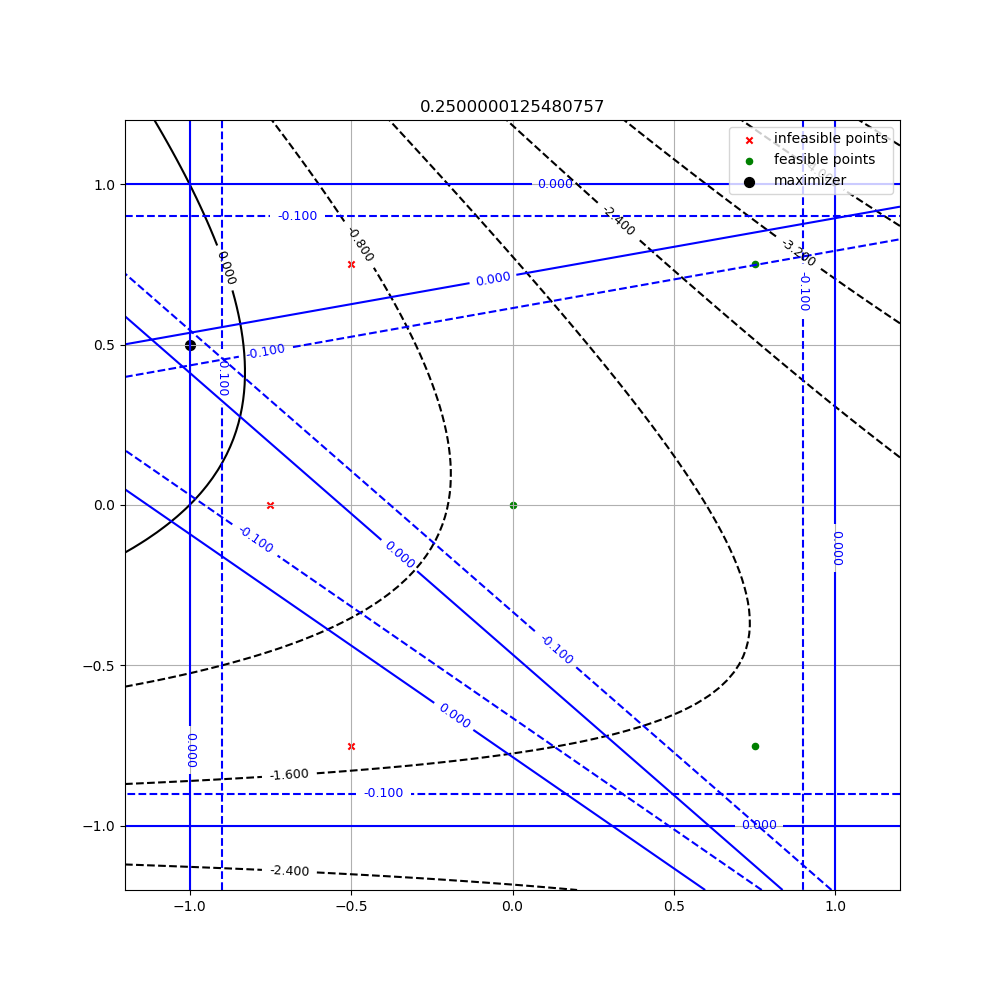
\includegraphics[width=300px]{images/pyomo_cut_solution.png}
    \caption{
		Adding linear cuts to remove infeasible points.
		Sample points that have already been evaluated and found to be feasible are shown as green circles.
		Attempted evaluations that resulted in infeasible evaluations are shown as red x's.
		The linear cuts (blue lines) are chosen to minimize the value of the objective (in black) while ensuring that all failed evaluations are infeasible.
	}
    \label{pvip}
\end{figure}


Suppose that the algorithm has evaluated several infeasible points after solving the trust region subproblem.
These are stored in a set $\trsinfset = \{n_1, n_2, \ldots, n_{|\trsinfset|}\}$.
We then choose one hyperplane $\{x \in \Rn | d_k^Tx = b_k\}$ for each infeasible point to remove that feasible point from our next attempt to solve the trust region subproblem.
Notice that these hyperplanes are \emph{decision variables} during the next attempt, so as to give as much freedom for our next trial solution.

If we let $\trstol \in (0, 1)$ be the percentage of the trust region radius with which we wish buffer our next solution, 
we arrive at the following optimization problem:
\begin{align}
\label{buffered_trust_region_subproblem}
\begin{array}{ccc}
\min_{s, d^{(k)} \in \Rn, b_i \in \reals}	& \mfk(x) & 	\\
 \mbox{subject to}  & n_k^Td^{(k)} \ge b_k + \trstol \dk& \forall 1 \le k \le |\trsinfset | \\
 & s^T d^{(k)} \le b_k &   \forall 1 \le k \le |\trsinfset |  \\
 & \|d^{(k)}\| = 1 & \forall 1 \le k \le |\trsinfset |	\\
 & \nabla \mcik(\xk) ^T s \le \mcik(\xk) & \forall 1 \le i \le m\\
 & \|s - \xk \|_{\infty} \le \dk & \\
\end{array}
\end{align}

We use this optimization problem as a subroutine of the trust region subproblem algorithm:

\begin{algorithm}[H]
    \caption{Solve Trust Region Subproblem}
    \label{linear_cut_trust_region_subproblem}
    \begin{itemize}
        \item[\textbf{Step 0}] \textbf{(Initialization)} \\
	    Initialize the set of infeasible points $\trsinfset = \emptyset$.
        
        \item[\textbf{Step 1}] \textbf{Solve Trust Region Problem} \\
	    Solve \cref{buffered_trust_region_subproblem} to find trial point $s$.
	    If the feasible set is empty, \textbf{Fail}
        
        \item[\textbf{Step 2}] \textbf{(Check feasibility)} \\
            Evaluate the objective and constraints $s$.
            If $s\in\feasible$, \textbf{return} $s$.
            Otherwise, if $s\in\feasible$ and $s \in \sampletrk$, \textbf{Fail}
	    Otherwise, if $s\in\feasible$ and $s \not \in \sampletrk$ \begin{itemize}
	    	\item[] $\trsinfset \gets \trsinfset \cup \{s\}$
	    	\item[] Go to Step 1
	    \end{itemize}
            
        \item[\textbf{Step 3}] \textbf{(Update maximum volume ellipsoid)} \\
	    Update $E_{max}$
	    decrease random search variance
            
        $k \gets k+1$ and go to Step 1.
    \end{itemize}
\end{algorithm}

The properties of the trial point found by this algorithm, as well as its convergence are detailed in \cref{efficiency_condition_analysis}.



\subsubsection{Decrease $\dk$}

Another option is to simply decrease the trust region radius.
However, in order to do this, we must be sure that we use a search region contained within $\feasible$ for small enough $\dk$.
We will later show that the set $\capcones$ defined in \cref{definecapcones} is just this set.
Thus, we can replace the trust region subproblem with

\begin{align*}
\begin{array}{ccc}
\min_{s^{(i)},x\in\Rn,t_i>0} & m_f(x) & \\
 & x = \wik + t _i s^{(i)} & 1 \le i \le m \\
 & \|s^{(i)}\| = 1 & 1 \le i \le m \\
 -\left(s^{(i)}\right)^T\hgik \ge \beta \dk^{\frac 1 2 } & 1 \le i \le m \\
\end{array}
\end{align*}
We will later show that a point within the feasible set for this optimization problem satisfies the efficiency condition.

% \begin{comment}
% Double check that this is the same as in the masters2.tex
% \end{comment}

% The optimization program for finding this constraint is given by:
% 
% A set of $u^i, 1 \le i \le n_{I}$ infeasible points.
% A set of $v^i, 1 \le i \le n_{F}$ feasible points.
% 
% The current Lagrange polynomial $\frac 1 2 x^T Q x + b^Tx$.
% Require all infeasible point to be a distance at least $d$ from the feasible region.
% 
% 
% Find a set of planes $(n^i, b^i), 1 \le i \le n_{P}$.
% 
% Require $n_P \ge n_I$.
% 
% Let $n_I$ be the number of infeasible points
% Tolerance $\delta$
% \begin{align}
% \begin{array}{ccc}
% \min_{s, d_i \in \Rn, b_i \in \reals}	& \mfk(x) & 	\\
%  \mbox{subject to}  & d_k^T n_k \ge b_i + \trstol & \forall 1 \le k \le |\trsinfset | \\
%  & d_k^T s \le b_i &   \forall 1 \le k \le |\trsinfset |  \\
%  & \|d_k\| = 1 & \forall 1 \le k \le |\trsinfset |	\\
%  & \nabla \mcik(\xk) ^T s \le \mcik(\xk) & \forall 1 \le i \le m\\
%  & \|s - \xk \|_{\infty} \le \dk & \\
% \end{array}
% \end{align}



\subsection{Recover Feasible Ellipsoid}

Although $\sampletrk$ will be feasible for small enough $\dk$, there may be some iterations in which it contains infeasible points.
When this happens, and a point we attempt to use as a sample point is infeasible, we decrease the trust region radius.
However, this means the previous sample points are no longer poised for the next iteration.
We then construct a feasible ellipsoid within the convex hull of the previous feasible points and the current iterate.

% \begin{algorithm}[H]
%     \caption{Restore a feasible ellipsoid}
%     \label{restore_feasible_ellipsoid}
%     \begin{itemize}
%         \item[\textbf{Step 0}] \textbf{(Initialization)} \\
%             Feasible ellipsoid, current iterate
%             
%         \item[\textbf{Step 1}] \textbf{(Construct Ellipsoid within the convex hull)} \\
%         	A sphere works.
%     \end{itemize}
% \end{algorithm}
% 
% \begin{comment}
% Fill this in.
% \end{comment}
% This is why we require an initial feasible ellipsoid.


To do this, we first construct the convex hull of the points 
Let $Y = y^{(0)}, y^{(1)}, \ldots, y^{(p)}$ be the set of sample points used in the previous iteration.

\begin{algorithm}[H]
    \caption{Restore a feasible ellipsoid}
    \label{compute_convex_hull}
    \begin{itemize}
        \item[\textbf{Step 0}] \textbf{(Initialization)} \\
            $P_{\textrm{planes}} = \emptyset$
            
        \item[\textbf{Step 1}] \textbf{(Potentially add hyperplane)} \\
	    For each subset $S \subseteq Y \cup \{x^{(k-1)}\}$ with $|S| = n - 1$, construct the hyplerplane $ax\le b$ running through the points $S \cup \xk$.
	    If the inequality $ap \le b$ is valid for each $p \in Y \cup \{x^{(k-1)}\}$, add the pair $(a, b)$ to $P_{\textrm{planes}}$.
	
	\item[\textbf{Step 1}] \textbf{(Construct ellipsoid)} \\
	   Construct the largest possible ellipsoid within $P_{\textrm{planes}} \cap \tr$
    \end{itemize}
\end{algorithm}


\subsection{Convergent Algorithm}

We can now state the algorithm.


\subsubsection{Psuedocode}

The algorithm depends on a parameter $p_{\Delta}$
\begin{align}
0 < p_{\Delta} < \min\{p_{\alpha}, p_{\beta}\} \le 1 \label{define_p_delta} 
\end{align}

\begin{algorithm}[H]
    \caption{Always-feasible Constrained Derivative Free Algorithm}
    \label{constrained_dfo}
    \begin{itemize}
        \item[\textbf{Step 0}] \textbf{(Initialization)} \\
            Initialize tolerance constants 
            $\tolcrit \ge 0$,
            $\tolrad \ge 0$,
            \color{red} starting point $x^{(0)} \in \feasible$  OR a starting feasible ellipsoid   \color{black},
            initial radius $\Delta_0 > 0$,
            iteration counter $k=0$,
            $0 < \omegadec < 1 \le \omegainc$,
            $0 < \gammasm < \gammabi \le 1$,
            $k \gets 1$,
            $0 < \omegadec < 1 \le \omegainc$,
            $0 < \gammasm < \gammabi < 1$,
            $0 < p_{\Delta} < \min\{p_{\alpha}, p_{\beta}\}$,
            $0 < \kappa_{\chi}$
            
        \item[\textbf{Step 1}] \textbf{(Construct the model)} \\
	    If $m_{f}^{k-1}(x)$, $m_{c_i}^{k-1}(x)$ exist, then use these to construct the feasible ellipsoid \cref{def_ellipse_k}.
	    If they do not, then run \cref{restore_feasible_ellipsoid} to construct a new $\sampletrk$ and $\dk$.
            Ensure that the sample points are poised with respect to $ \sampletrk $ for \cref{accuracy} by calling \cref{model_improving_algorithm} on the shifted ellipsoid.
            Construct $\mfk$ and $\mcik$ as described in \cref{reg}.
        
        \item[\textbf{Step 2}] \textbf{(Check stopping criteria)} \\
            Compute $\chi_k$ as in \cref{critical}. \begin{itemize}
                \item[] If $ \chik < \tau_{\xi} $ and $\dk <\tau_{\Delta}$ then return $\xk$ as the solution.
                \item[] Otherwise, if $\kappa_{\chi} \dk^{p_{\Delta}} > \chik$ then 
                $\Delta_{k+1} \gets \omegadec\dk$, 
                $x^{(k+1)} \gets \xk$,
                $k \gets k+1$ and go to Step 1.
            \end{itemize}
        
        \item[\textbf{Step 3}] \textbf{(Solve the trust region subproblem)} \\
        	Use \cref{linear_cut_trust_region_subproblem} to solve the trust region subproblem.
        	If \cref{detect_infeasible_trust_region_subproblem} is not satisfied, then reduce the trust region $\Delta_{k+1} = \omegadec\dk$, $k \gets k+1$ and go to Step 1.
            
        \item[\textbf{Step 4}] \textbf{(Test for improvement)} \\
            Evaluate $f(\xk + \sk)$ and evaluate $\rho_k$ as in \cref{rho} \begin{itemize}
                \item[] If $\rho_k < \gammasm$ then $\xkpo=\xk$ (reject) and $\Delta_{k+1} = \omegadec\dk$
                \item[] If $\rho_k \ge \gammasm$ and $\rho < \gammabi$ then $\xkpo=\xk+\sk$ (accept), $\Delta_{k+1} = \omegadec\dk$
                \item[] If $\rho_k > \gammabi$ then $\xkpo=\xk+\sk$ (accept), $\Delta_{k+1} = \omegainc\dk$
                % and either increase the radius or decrease if $\nabla \mfk(\xk)$ is small
            \end{itemize}
            $k \gets k+1$ and go to Step 1.
    \end{itemize}
\end{algorithm}

\section{Convergence Analysis}

\subsection{Assumptions}
Our convergence analysis follows closely that of \cite{Conejo:2013:GCT:2620806.2621814}.
Throughout our assumptions, we will let $\Omega$ be some open region containing $\feasible$.

\paragraph{Bounded functions}
The following assumptions let us know that the functions $f$ and $c_i \forall 1 \le i \le m$ are smooth functions.



\begin{assumption}
\label{bounded_below}
The function $f$ is bounded below in $ \Omega $. That is, there exists an $\fmin$ such that
\begin{align}
f(x) \ge \fmin \quad  \forall x \in \Omega
\end{align}
\end{assumption}


\begin{assumption}
\label{bounded_gradient_constraint}
The functions $c_i$ has bounded gradient  in $ \Omega $. That is, there exists an $\gcmax > 0$ such that
\begin{align}
\|\nabla c_i(x)\| \le \gcmax \quad  \forall x \in \Omega\forall 1 \le i \le m
\end{align}
\end{assumption}

\begin{assumption}
\label{bounded_constraint_hessians}
Each function $c_i$ for $1 \le i \le m$ is has bounded hessian. That is, there exists a $ \maxconstrainthessian $ such that:
\begin{align}
\|\nabla^2 c_i(x) \| \le \maxconstrainthessian \quad \forall x \in \Omega \label{bounded_hessians}
\end{align}
\end{assumption}

\begin{assumption}
\label{maxnormassumption}
There exists a $\maxnorm > 0$ such that for each $k \in \ints$ we have
\begin{align*}
\|x\| \le \maxnorm \forall x \in \feasiblek
\end{align*}
\end{assumption}

\begin{assumption}
\label{bounded_hessians}
The matrices $\hk$ are uniformly bounded, that is, there exists a constant $ \hfb \ge 1 $ such that 
\begin{align}
\|\hk\| \le \hfb - 1 \quad \forall k \ge 0.
\end{align}
\end{assumption}

\paragraph{All functions are smooth}
The following assumptions let us know that the functions $f$ and $c_i \forall 1 \le i \le m$ are smooth functions.


\begin{assumption}
\label{lipschitz_gradient}
The function $f$ is differentiable and its gradient $\nabla f$ is Lipschitz continuous with constant $L_g > 0$ in $ \Omega $.
\begin{align}
\|\nabla f(x) - \nabla f(y)\| \le L_g \|x - y\| \quad \forall x,y \in \Omega.
\end{align}
\end{assumption}

\begin{assumption}
\label{lipschitz_constraints}
Each function $c_i$ for $1 \le i \le m$ is differentiable and its gradient $\nabla c_i$ is Lipschitz continuous with constant $\lpc$ in $\Omega$:
\begin{align}
\|\nabla c_i(x) - \nabla c_i(y)\| \le \lpc \|x - y\| \label{def_lipshitz}
\end{align}
\end{assumption}


\begin{assumption}
\label{lipschitz_hessian}
The function $f$ is twice differentiable and its hessian $\nabla^2 f$ is Lipschitz continuous with constant $L_h > 0$ in $ \Omega $:
\begin{align}
\|\nabla^2 f(x) - \nabla^2 f(y)\| \le L_h \|x - y\| \quad \forall x,y \in \Omega.
\end{align}
\end{assumption}


\paragraph{Regularity Assumptions}
We use the following assumptions as our regularity assumptions.

\begin{assumption}
\label{minangleassumption}
There exists a $\minangledelta > 0$ and a $\minanglealpha > 0$ such that for each $x \in \Omega$ there exists a $u \in \Rn$ with $\|u\| = 1$ such that 
if $\dk \le \minangledelta$ and $i$ is such that 
$\zik \in B_{\infty}(\xk, 3\sqrt{n}\dk)$
then
\begin{align*}
-\frac {\gmcik}{\|\gmcik\|} ^Tu \ge \minanglealpha.
\end{align*}
\end{assumption}


\begin{assumption}
\label{mingradassumption}
There exists a $\mingradepsilon > 0$ and a $\mingrad > 0$ such that for each $x \in \Omega$ we have
\begin{align*}
-c_i(x) \le \mingradepsilon \Longrightarrow \| \nabla c_i(x) \| \ge \mingrad.
\end{align*}
\end{assumption}

\begin{assumption}
\label{minactivegradassumption}
There is a lower bound on the gradient at $x$ of any constraint $c_i$ whose linearization is nearly active an the projection of $x - \nabla f(x)$.

That is, 
there exist constants $\minactivegrad > 0$ and $\minactivegraddelta > 0$
such that for all $x \in \Omega$,
after defining
\begin{align}
\mathcal F_x = \{ y \in \Rn | c_i(x) + \nabla c_i(x)^T(y - x) \le 0 \quad \forall 1 \le i \le m\}, \nonumber \\
p_x = \argmin_{p \in \mathcal F_x} \|x - \nabla f(x) - p\|^2, \nonumber \\
\mathcal A_x = \{1 \le i \le m | \left|c_i(x) + \nabla c_i(x)^T(p_x - x)\right| \le \minactivegraddelta \} \label{define_projection_active}
\end{align}
then
\begin{align*}
\left\|\nabla c_i(x)\right\| \ge \minactivegrad \quad \forall i \in \mathcal A_x.
\end{align*}
\end{assumption}


\paragraph{Proven assumptions}
The following assumptions are proven throughout the paper.

\begin{assumption}
\label{hopefully_there_is_a_bound_for_this}
We have that $\Gamma_0(A_k) \le M_{\Gamma_0} \forall k$
\color{red}
This follows from continuity?
\color{black}
\end{assumption}


% \begin{assumption}
% \label{h4_placeholder}
% The iterates are generated by the algorithm.
% That is,
% \begin{itemize}
% \item something about $\mfk$
% \item something about $\xk$
% \item whatever else needs to be said
% \end{itemize}
% \end{assumption}


\begin{assumption}
\label{accuracy_assumption}
There exists a constant $\kappa_g$ such that 
\begin{align}
\|\nabla f(\xk) - \nabla \mfk(\xk) \| \le \kappa_g \dk^2 \\
\|\nabla c_i(\xk) - \gmcik \| \le \kappa_g \dk^2 \quad \forall 1 \le i \le m
\end{align}
\end{assumption}
This is the accuracy condition \cref{accuracy} and is shown in \cref{accuracy_is_satisfied}.


\begin{assumption}
\label{bounded_gradient}
The function $f$ has bounded gradient in $ \Omega $. That is, there exists an $\gfmin > 0$ such that
\begin{align}
\|\nabla f(x)\| \le \gfmin \quad  \forall x \in \Omega
\end{align}
\end{assumption}
This follows immediately from \cref{lipschitz_gradient} and \cref{maxnormassumption}.


\begin{assumption}
\label{ellipsoids_exist}
There exists an $n\times n$, symmetric, positive-definite matrices $\qk$, vectors $\ck \in \Rn$, and a bound $\sigma_{\text{min}} > 0$ and scalars $\delta_k > 0$
such that each of the following hold:
\begin{itemize}
\item The condition numbers of $\qk$ are bounded:
\begin{align}
\sigma(Q^{(k)}) \le \sigma_{\text{max}} \forall k \in \ints
\end{align}
\item An ellipsoid defined by $\qk, \ck$ is feasible:
\begin{align}
\unshiftedellipsoid \subseteq \feasiblek \cap \tr
\end{align}
where
\begin{align}
\unshiftedellipsoid = \left\{x \in \Rn | \left(x - \ck \right)^T \qk \left(x - \ck\right) \le \frac 1 2 {\delta_k}^2 \right\}
\end{align}
\item An ellipsoid defined by $\qk, \ck$ is close to the current iterate:
\begin{align}
\xk \in \scaledunshiftedellipsoid
\end{align}
where
\begin{align}
\scaledunshiftedellipsoid = \left\{x \in \Rn | \left(x - \ck\right)^T \qk \left(x - \ck\right) \le {\delta_k}^2 \right\}
\end{align}
\end{itemize}
\end{assumption}

We have already constructed $\qk$, $\ck$, $\delta_k$, and we show that they satisfy \cref{ellipsoids_exist} in \cref{feasible_ellipsoid_analysis}.


We will be using the following result shown \cite{Billups_Larson_2013}, Corollary 4.7.
We restate the theorem here, with the simplication that $f$ is deterministic function.
Note that the assumption is satisfied for $f$ by \cref{lipschitz_hessian}, and for the constraints by \cref{bounded_constraint_hessians}.

\begin{assumption}
\label{fully_quadratic_assumption}
Suppose that a set $S$ and a radius $\dmax$ are given.
Assume that $f$ is twice continuously differentiable with Lipshcitz continuous Hessian in an open domain containing the $\dmax$ neighborhood
$\cup_{x \in S} B(x; \dmax)$ of the set $S$.
\end{assumption}

\begin{lemma}
\label{change_radius} 
Let $Y$ be a poised set of $p$ points, and let $R = \max_{i}\|y^i - y^0\|$.
Let $f$ satisfy \cref{fully_quadratic_assumption} over some convex set $\Omega$, and let $m(x)$ denote the quadratic model of $f$ using \cref{reg}.
If $f$ is a Lipschitz continuous function with Lipschitz constant $L_g$, and $m_f(x)$ is a quadratic model of $f$.
Then, there exist constrants $\Lambda_1, \Lambda_2, \Lambda_3$ independent of $R$ such that for all $x \in B(y^0, R)$,
\begin{align*}
\|f(x) - m_f(x)\| \le 4\Lambda_1 R^3L \sqrt{p+1} \\
\|\nabla f(x) - \nabla m(x)\| \le 4\Lambda_2R^2  L \sqrt{p+1} \\
\|\nabla^2 f(x) - \nabla^2 m(x)\| \le 4\Lambda_3  RL \sqrt{p+1}
\end{align*}
\end{lemma}


We also use a theorem found within our convergence analysis for linear constraints:
\begin{theorem}
\label{shifted_ellipsoid}
Given $\qk$, $\ck$ as defined in \cref{ellipsoids_exist},
Let $\qk = L D^2 L^T$ where $L^TL = I$ and $D$ is a diagonal matrix with positive entries be the eigen-decomposition of $\qk$.
Also, let $\delta = \max_{x\in \ellipsek}\|x-c\|$, 
and define the transformation $T(x) = \delta DL^T(x - c)$.
Let $\hat m_f(u)$ be a model of the shifted objective $\hat f(u) = f(T^{-1}(u))$ in the $\delta$ ball such that
there exist constants $\kappa_{ef}, \kappa_{eg}, \kappa_{eh} > 0$ such that for all $\{u \in R^n | \;\|u\| \le \delta \}$, we have
% for all $u \in B(0 ; \delta)$ we have the following error bounds:
\begin{align*}
|\hat m_f(u) - \hat f(u)| \le \kappa_{ef} \delta^3\\
\|\nabla \hat m_f(u) - \nabla \hat f(u)\| \le \kappa_{eg}\delta^2\\
\|\nabla^2 \hat m_f(u) - \nabla^2 \hat f(u)\| \le \kappa_{eh}\delta.
\end{align*}

Then, with
\begin{align*}
\kappa_{ef}' = \kappa_{ef} \\
\kappa_{eg}' = \kappa_{eg}\sqrt{\kappa(\qk)} \\
\kappa_{eh}' = \kappa_{eh}\kappa(\qk),
\end{align*}
we have that for all $x \in \ellipsek$,
the model function $m_f(x) = \hat m_f(T(x))$ will satisfy
\begin{align*}
| m(x) - f(x)| \le \kappa_{ef}'\delta^3 \\
\|\nabla  m(x) - \nabla  f(x)\| \le \kappa_{eg}'\delta^2 \\
\|\nabla^2 m(x) - \nabla^2 f(x)\| \le \kappa_{eh}'\delta.
\end{align*}
\end{theorem}

\paragraph{Sufficient Reduction}
To ensure sufficient reduction of the objective's model function during each iteration, the authors of \cite{Conejo:2013:GCT:2620806.2621814} impose the following efficiency condition:
\begin{equation}
\label{efficiency}
\mfk(\xk) - \mfk(\xk + \sk) \ge \kappa_f \chi_k \min\left\{ \frac{\chi_k}{1+\|\nabla^2 \mfk(\xk)\|}, \dk, 1 \right\}
\end{equation}
where $\kappa_f$ is a constant independent of $k$.
This is widely used within trust region frameworks such as \cite{Conejo:2013:GCT:2620806.2621814} and \cite{Conn:2000:TM:357813}.
It can be shown that the \emph{generalized Cauchy point} satisfies this condition \cite{Conn:2000:TM:357813}.


% A efficiency condition \cref{efficiency} is satisfied:
% \begin{equation}
% \mfk(\xk) - \mfk(\xk + \sk) \ge \kappa_f \chi_k \min\{ \frac{\chi_k}{1+\|\nabla^2 \mfk(\xk)\|}, \Delta_k, 1 \}
% \end{equation}

With explicit constraints, we know that this is satisfied by the Generalized Cauchy Point.
For convex constraints, we use the minimization within the buffered feasible region.
However, we show that this is not required during every iteration, but those iterations in which $\chik \ge \kappa_{\Delta}\dk^{p_{\Delta}}$.
This is the topic of \cref{sufficient_reduction_section}.


\subsection{Accuracy}
\label{ellipsoidal_lambda}

\begin{theorem}
\label{accuracy_is_satisfied}
Suppose that \cref{fully_quadratic_assumption} and \cref{ellipsoids_exist} holds.
Then, the accuracy condition \cref{accuracy_assumption} is satisfied for each iterate $k$ with $\dk \le 1$.
\end{theorem}

\begin{proof}
Fix an iterate $k$.
We can use \cref{ellipsoids_exist} to define $\qk, \ck, \scaledunshiftedellipsoid$.
As in \cref{shifted_ellipsoid}, we can give $\qk = LD^2L^T$ its eigen-decomposition, and define $\delta = \max_{x \in \unshiftedellipsoid} \|x - \mu^{(k)}\|$, 
so the transformation $T(x) = \delta D L^T(x - \mu^{(k)})$ maps $E^{(k)}$ to the $\delta$ ball.
As also described in \cref{shifted_ellipsoid}, we  create shifted functions
\begin{align*}
\begin{array}{ccc}
\hat {m}_f(u) = m_f(T^{-1}(u)),&  \hat f (u) = f(T^{-1}(u)) &\\
\hat {m}_{c_i}(u) = m_{c_i}(T^{-1}(u)), &  \hat c_i (u) = c(T^{-1}(u))& \forall 1 \le i \le m
\end{array}
\end{align*}
After using \cref{model_improving_algorithm} to choose sample points, we know by \cref{quadratic_errors} that
here exists a constants $\kappa_f, \kappa_g, \kappa_h$ such that for all $u \in B_2(0, \delta)$ and all $1\le i\le m$:
\begin{align*}
\begin{array}{ccc}
\left\| \hat {f}\left(u\right) -  \hat{m}_f\left(u\right) \right\|\le \kappa_f \delta^3 &
\left\|\nabla \hat {f}\left(u\right) - \nabla \hat{m}_f\left(u\right) \right\|\le \kappa_g \delta^2 &
\left\|\nabla^2 \hat {f}\left(u\right) - \nabla^2 \hat{m}_f\left(u\right) \right\|\le \kappa_h \delta \\
\left\| \hat {{c_i}}\left(u\right) -  \hat{m}_{c_i}\left(u\right) \right\|\le \kappa_f \delta^3 &
\left\|\nabla \hat {{c_i}}\left(u\right) - \nabla \hat{m}_{c_i}\left(u\right) \right\|\le \kappa_g \delta^2 &
\left\|\nabla^2 \hat {{c_i}}\left(u\right) - \nabla^2 \hat{m}_{c_i}\left(u\right) \right\|\le \kappa_h \delta.
\end{array}
\end{align*}
We can then use \cref{change_radius} to conclude that there is another constant $\Lambda_2$ such that for all $u \in B_2(0, 2\delta)$:
\begin{align*}
\left\|\nabla \hat {f}\left(u\right) - \nabla \hat{m}_f\left(u\right) \right\|\le 4 \Lambda_2 \left(2\delta\right)^2 L \sqrt{p+1} = {\kappa'}_g\delta^2, \quad \textrm{and} \quad
\left\|\nabla \hat {c_i}\left(u\right) - \nabla \hat{m}_{c_i}\left(u\right) \right\|\le {\kappa'}_g\delta^2.
\end{align*}
where $\kappa_{g}' = 16 \Lambda_2 L \sqrt{p+1}$.
After defining $\kappa''_{g} =  \sigma_{\text{max}}\kappa'_g$, we see that
we can use  \cref{shifted_ellipsoid} to conclude that for all $x_0 \in \scaledunshiftedellipsoid$:
\begin{align*}
\left\|\nabla f\left(x_0 \right) - \nabla m_f\left(x_0\right)\right\| \le 
\kappa'_g  \dk^2 \sqrt{\kappa\left(\frac 2 {\delta_k} Q^{(k)}\right)} \le \kappa'_g \sqrt{\sigma_{\text{max}}}\dk^2 \le \kappa''_g\dk^2 \\
\left\|\nabla {c_i}\left(x_0 \right) - \nabla m_{c_i}\left(x_0\right)\right\| \le \kappa''_g\dk^2 \quad \forall 1 \le i \le m
\end{align*}
In particular, $\xk \in \scaledunshiftedellipsoid$.
\end{proof}


% Notice that Lemma 3.1 and Lemma 3.2 within \cite{doi:10.1080/10556788.2015.1026968} show that $\lim_{k\to\infty}\dk = 0$ without requiring the accuracy condition.
% This is because Lemma 3.1 assumes that $\dk \le 1$ explicitly, while Lemma 3.2 uses the accuracy of the model's hessians.
% This justifies the use of a $\dmax > 0$, such that $\dk \le \dmax\;\forall k \in \naturals$.


\subsection{Construction of $\sampletrk$}
\label{feasible_ellipsoid_analysis}

\subsubsection{Notation}
Then for all $1 \le i \le m$, $k = 1, \ldots$, define the following whenever they exist:

% \theta^{\text{min}} = \liminf_{k\to\infty} \theta^{\text{min}}_k \label{def_theta_min} \\
% \theta^{\text{max}} = \limsup_{k\to\infty} \theta^{\text{max}}_k \label{def_theta_max} \\
\begin{align}
\bs = \sqrt{ 1 - (\theta^{\text{max}}_k)^2} \label{def_bs} \\
0 < g_{\text{low}} \le \|\gmcik\| \le g_{\text{hi}} \label{def_g_bounds} \\
0 < h_{\text{low}} \le \|\nabla^2m_{c_i}(x)\| \le h_{\text{hi}} \label{def_h_bounds} \\
\nabla c_i(\xk) = \nabla m_{c_i}(\xk) + \epsilon_{g}\dk^2\nu \label{def_lambda_poised} \\
\inf_{k}\min\{\sigma(\nabla c_{\mathcal I_k}(\xk)) \; | \; \sigma(\nabla c_{\mathcal I_k}(\xk)) > 0 \} \ge \epsilon_{\sigma} > 0\\
\end{align}


\subsubsection{Existence Proof}


\begin{lemma}
\label{cone_subset_cone}
Given $u, v \in \rn$, and $\gamma, \beta \in (0, 1]$ that satisfy $\|u\| = \|v\|= 1$, $u^Tv = \gamma > \beta > 0$, define
\begin{align*}
B = \{x\in\rn | {v}^Tx \ge \beta\|x\|\}, \quad
S = \left\{x\in\rn \bigg| v^Tx \ge \left(\beta\gamma + \sqrt{(1 - \beta^2)\left(1 - \gamma^2\right)}\right)\|x\| \right\}. 
\end{align*}
Then, $S \subseteq B$.
\end{lemma}



\begin{proof}
For a contradiction, let $y \in \rn$ be such that $y \not \in B$ and $y \in S$ and define $\hat y = \frac{y}{\|y\|}$.
That is,
\begin{align}
v^T\hat y < \beta \label{csc_vy} \\
u^T\hat y \ge \beta\gamma + \sqrt{\left(1 - \beta^2\right)\left(1 - \gamma^2\right)}. \label{csc_uy}
\end{align}

Define
\begin{align*}
x^{\star} = \beta v + \sqrt{\frac{1 - \beta^2}{1 - \gamma^2}} (u - \gamma v )
\end{align*} and notice that
\begin{align}
\begin{array}{ccccc}
{u}^Tx^{\star} &=& \beta\gamma + \sqrt{\frac{1 - \beta^2}{1 - \gamma^2}} (1 - \gamma^2) &=&  \beta\gamma + \sqrt{\left(1 - \beta^2\right)\left(1 - \gamma^2\right)} \\
{v}^Tx^{\star} &=& \beta + \sqrt{\frac{1 - \beta^2}{1 - \gamma^2}}(\gamma - \gamma) &=& \beta \\
{x^{\star}}^Tx^{\star} &=& \beta^2 + 2\beta\sqrt{\frac{1 - \beta^2}{1 - \gamma^2}}(\gamma - \gamma) + \frac{1 - \beta^2}{1 - \gamma^2} (1- 2\gamma^2 + \gamma^2)&=& 1.
\end{array}. \label{csc_vx_ux}
\end{align}

Using \cref{csc_vx_ux} and \cref{csc_uy}, we see that
\begin{align*}
\beta\gamma + \sqrt{\left(1 - \beta^2\right)\left(1 - \gamma^2\right)} \le {u}^T\hat y = {u}^T\left(x^{\star} + \hat y - x^{\star}\right) 
= \beta \gamma + \sqrt{(1 - \beta^2)\left(1 - \gamma^2\right)} + {u}^T\left(\hat y - x^{\star}\right).
\end{align*}
Subtracting $\beta\gamma + \sqrt{\left(1 - \beta^2\right)\left(1 - \gamma^2\right)}$ from both sides, we find that
\begin{align}
{u}^T\left(\hat y - x^{\star}\right) \ge 0 \label{csc_uymx}.
\end{align}
Likewise, we can use \cref{csc_vx_ux} and \cref{csc_vy} to provide
\begin{align*}
\beta > {v}^T\hat y = {v}^T\left(x^{\star} + \hat y - x^{\star}\right) = \beta + {v}^T\left(\hat y - x^{\star}\right).
\end{align*}
After subtracting $\beta$ from both sides, we see
\begin{align}
{v}^T\left(\hat y - x^{\star}\right) < 0 \Longrightarrow -{v}^T\left(\hat y - x^{\star}\right) > 0. \label{csc_vymx}
\end{align}
% which means $\hat y \ne x^{\star}$.

Lastly, we will need
\begin{align}
\gamma > \beta 
\Longrightarrow 1 - \beta^2 > 1 - \gamma^2
\Longrightarrow \sqrt{\frac{1 - \beta^2}{1 - \gamma^2}} > 1
\Longrightarrow \gamma \sqrt{\frac{1 - \beta^2}{1 - \gamma^2}} - \beta > 0. \label{csc_gamma_beta_positive}
\end{align}

Now, we can compute
\begin{align*}
{\left(\hat y - x^{\star}\right)}^Tx^{\star} = 
\beta {\left(\hat y - x^{\star}\right)}^Tv
+ \sqrt{\frac{1 - \beta^2}{1 - \gamma^2}} 
\left(u^T\left(\hat y - x^{\star}\right) - \gamma v^T \left(\hat y - x^{\star}\right) \right)\\ 
= \left[\gamma \sqrt{\frac{1 - \beta^2}{1 - \gamma^2}} - \beta\right] \left[-v^T\left(\hat y - x^{\star}\right)^T\right]
+ \left[\sqrt{\frac{1 - \beta^2}{1 - \gamma^2}}\right] \left[u^T\left(\hat y - x^{\star}\right) \right] > 0.
\end{align*}
because \cref{csc_uymx}, \cref{csc_vymx}, and \cref{csc_gamma_beta_positive} show that the first product is postive and the second product is non-negative.
However, this is a contradiction as
\begin{align*}
1 = \|\hat y\|^2 = \|x^{\star} + \hat y - x^{\star}\|^2 = \|x^{\star}\|^2 + 2{\left(\hat y - x^{\star}\right)}^Tx^{\star} + \|\hat y - x^{\star}\|^2 > \|x^{\star}\|^2 = 1
\end{align*}
and there is no such $y$.
Thus, any $y \in\rn$ with $y \in S$ must also have $y \in B$.
\end{proof}

\begin{lemma}
\label{only_small_z_matters}
Assume \cref{mingradassumption}, \cref{bounded_gradient_constraint}, \cref{bounded_constraint_hessians}, \cref{accuracy_assumption} hold.
Define
\begin{align}
\mingraddelta = \min\left\{
1,
\sqrt{\frac 1 {2\kappa_g} \mingrad},
\sqrt{\frac 1 {2\kappa_g} \gcmax},
\frac{\mingradepsilon}{\frac 3 2 \gcmax\sqrt{n} + nM},
\sqrt{\frac{2\mingradepsilon}{\mingrad}}
\right\} \label{define_mingraddelta}
\end{align}
and suppose that
\begin{align}
\dk \le \mingraddelta \label{szm_delta_small}.
\end{align}

Then either $c_i(y) \le 0 \quad \forall y \in \tr$ or both $\zik \in \tr$ and $\left\|\gmcik\right\| > \frac 1 2 \mingrad$.

\end{lemma}

\begin{proof}
Let $y\in \tr$. Because $m_{c_i}$ is fully quadratic, we know that there exists a $\kappa_g$ such that
\begin{align*}
\left\|\nabla c_i(x) - \gmcik\right\| \le \kappa_g \dk^2.
\end{align*}
Using \cref{bounded_constraint_hessians}, we also know that
\begin{align*}
c_i(y) \le c_i(\xk) + \left(\gmcik\right)^T(y - \xk) + \frac 1 2 \left(y - \xk\right)^T\nabla^2{c_i}(\xk)\left(y - \xk\right) \\
\le c_i(\xk) + \|\gmcik\|\sqrt{n}\dk +nM\dk^2.
\end{align*}

\emph{Case 1}
Suppose that $-m_{c_i}(\xk) \ge \mingradepsilon \Longrightarrow -c_i(\xk) \ge \mingradepsilon$.
Then  by \cref{bounded_gradient_constraint} and \cref{szm_delta_small}, we know that 
$\| \gmcik \| \le \left\|\nabla c_i(\xk)\right\| + \kappa_g \dk^2 \le \frac 3 2 \gcmax$.
But by \cref{szm_delta_small}, we have that
\begin{align*}
\frac 3 2 \gcmax\sqrt{n}\dk + nM\dk^2 \le \left(\frac 3 2 \gcmax\sqrt{n} + nM\right)\dk \le \mingradepsilon \\
\Longrightarrow \|\gmcik\|\sqrt{n}\dk + nM\dk^2 \le \frac 3 2 \gcmax\sqrt{n}\dk + nM\dk^2 \le \mingradepsilon \le -c_i(\xk)\\
\Longrightarrow c(y) \le c_i(\xk) + \|\gmcik\|\sqrt{n}\dk + nM\dk^2 \le 0.
\end{align*}

\emph{Case 2}
Suppose that $-m_{c_i}(\xk) \le \mingradepsilon \Longrightarrow -c_i(\xk) \le \mingradepsilon$.
Then, by \cref{mingradassumption}, $\|\nabla c(\xk) \| \ge \mingrad \Longrightarrow \|\gmcik\| \ge \mingrad - \kappa_g \dk^2 \ge \frac 1 2 \mingrad > 0$.
By \cref{szm_delta_small}, this means that 
\begin{align*}
\|\zik-\xk\| = \frac{-c(\xk)}{\left\|\gmcik\right\|^2} \le \frac{2\mingradepsilon}{\mingrad}\le \dk^2 \le \dk \Longrightarrow \zik \in \tr.
\end{align*}
\end{proof}


\begin{lemma}
\label{each_constraints_cone_is_feasible}
Assuming \cref{mingradassumption}, \cref{bounded_gradient_constraint}, \cref{accuracy_assumption}, and \cref{bounded_constraint_hessians} hold,
if 
\begin{align}
\dk \le \min\left\{
1,
\mingraddelta,
\left(\frac{\alpha \mingrad}{2 \maxconstrainthessian \sqrt{n} + \epsilon_g}\right)^{\frac 1 {1-p_{\alpha}}},
\left(\frac{\beta}{4\epsilon_{g}}\mingrad\right)^{\frac 1 {2 - p_{\beta}}},
\left[\frac {\mingrad  \beta} {4\maxconstrainthessian\sqrt{n}\left(1 + \frac {\lpc} \maxconstrainthessian \right)}\right]^{\frac1 {1 - p_{\beta}} }
\right\}, \label{delta_is_small_enough}
\end{align} then
\begin{align*}
c_i(y) \le 0 \quad \forall y \in \fik \cap \tr.
\end{align*}
\end{lemma}

\begin{proof}

Because $\dk \le \mingraddelta$, we satisfy the assumptions for \cref{only_small_z_matters}.
If $c(y) \le \forall y \in \tr \subseteq \fik \cap \tr$ we are done.
From here on, we can assume both
\begin{align}
\zik \in \tr, \quad \textrm{and} \quad \left\|\gmcik\right\| \ge \frac 1 2 \mingrad. \label{z_is_active}
\end{align}
Let
\begin{align}
y = \wik + ts \in \fik \cap \tr \label{t_is_bounded}
\end{align}
with $t > 0, \|s\| = 1, -s^T\hgik \ge \beta \dk^{p_{\beta}}$.
By \cref{accuracy_assumption}, we know that there exists a $\nu\in\rn$ such that \cref{def_lambda_poised} holds with $\|\nu\|\le 1$:
\begin{align}
\nabla c_i(\xk) = \nabla m_{c_i}(\xk) + \epsilon_{g}\dk^2\nu. \label{model_error_for_gradient}
\end{align}

We know from \cref{bounded_constraint_hessians} that for all $x \in \tr$,
\begin{align}
c_i(x) \le c_i(\xk) + \nabla c_i(\xk)^T(x - \xk) + \maxconstrainthessian \left \|x - \xk \right\|^2 \label{constraint_lower_bound}
\end{align}

First, we will show that $c(\wik) \le 0$.
For simplicity, we use \cref{def_z}, and \cref{def_w} to compute
% \begin{align}
% \wik - \xk = \xk + \left(1 - \alpha \dk^{\frac 1 2 }\right)\left(\zik - \xk\right) - \xk 
% = \left(1 - \alpha \dk^{\frac 1 2 }\right)\left(\zik - \xk\right) \\
% =  \left(1 - \alpha \dk^{\frac 1 2 }\right)\left(\xk - \frac{c_i(\xk)}{\|\gmcik\|^2}\gmcik - \xk\right) 
% = \left(1 - \alpha \dk^{\frac 1 2 }\right)\frac{-c_i(\xk)}{\|\gmcik\|^2}\gmcik. \label{simple_computation}
% \end{align}


\begin{align}
\wik - \xk = \left(1 - \alpha \dk^{p_{\alpha} }\right)\frac{-c_i(\xk)}{\|\gmcik\|^2}\gmcik. \label{simple_computation}
\end{align}

Also, note by \cref{delta_is_small_enough}, \cref{def_alpha_beta}, \cref{def_p_alpha}, and $\dk^{1 - p_{\alpha}} \ge \dk^{2 - p_{\alpha}}$ that both
\begin{align*}
\dk^{1-p_{\alpha}} \le \frac{\alpha \|\gmcik\|}{\maxconstrainthessian \sqrt{n} + \epsilon_g} \Longrightarrow 
\maxconstrainthessian \sqrt{n}\dk^{1- p_{\alpha}} + \epsilon_g \dk^{2 - p_{\alpha}} \le \alpha \|\gmcik\| \quad \text{and} \quad
0 < 1 - \alpha \dk^{p_{\alpha}} < 1.
\end{align*}
Combine these along with \cref{z_is_active} to find 
\begin{align*}
\maxconstrainthessian \sqrt{n}\dk^{1-p_{\alpha}}\left(1 - \alpha \dk^{p_{\alpha}}\right)^2  + \epsilon_g \dk^{2 - p_{\alpha}} \left(1 - \alpha \dk^{p_{\alpha}}\right)
\le \maxconstrainthessian \sqrt{n}\dk^{1 - p_{\alpha}} + \epsilon_g \dk^{2 - p_{\alpha}} \le \alpha \|\gmcik\| \\
\end{align*}
Multiplying by $\dk^{p_{\alpha}}$ we see,
\begin{align*}
-\alpha \dk^{p_{\alpha}}\|\gmcik\| + M \left(1 - \alpha \dk^{p_{\alpha}}\right)^2 \sqrt{n}\dk+ \epsilon_g \dk^2 \left(1 - \alpha \dk^{p_{\alpha}}\right) \le  0.
\end{align*}
Multiplying by $-\frac{c_i(\xk)}{\|\gmcik\|} > 0$ and using $\zik \in \tr \Longrightarrow \frac{-c_i(\xk)}{\|\gmcik\|} \le \sqrt{n}\dk$, we see
\begin{align*}
-\alpha \dk^{p_{\alpha}}\|\gmcik\|\left(-\frac{c_i(\xk)}{\|\gmcik\|}\right) + M \left(1 - \alpha \dk^{p_{\alpha}}\right)^2 \left(-\frac{c_i(\xk)}{\|\gmcik\|}\right)^2\\
+\epsilon_g \dk^2 \left(1 - \alpha \dk^{p_{\alpha}}\right)\left(-\frac{c_i(\xk)}{\|\gmcik\|}\right) \le 0.
\end{align*}
Cancelling terms, we see
\begin{align*}
0 \ge \alpha \dk^{p_{\alpha}} c_i(\xk) + M \frac {c_i(\xk)^2}{\|\gmcik\|^2}\left(1 - \alpha \dk^{p_{\alpha}}\right)^2 + \epsilon_g \dk^2 \left(1 - \alpha \dk^{p_{\alpha}}\right)\frac{-c_i(\xk)}{\|\gmcik\|}.
\end{align*}
Because the last term is positive, we can only decrease the expression by multiplying by $\nu^T \frac{\gmcik}{\|\gmcik\|} \le 1$:
\begin{align*}
0\ge \alpha \dk^{p_{\alpha}} c_i(\xk) + M \frac {c_i(\xk)^2}{\|\gmcik\|^2}\left(1 - \alpha \dk^{p_{\alpha}}\right)^2 + \epsilon_g \dk^2 \left(1 - \alpha \dk^{p_{\alpha}}\right)\frac{-c_i(\xk)}{\|\gmcik\|^2}\nu^T\gmcik
\end{align*}
Using \cref{simple_computation}, this is
\begin{align*}
0 \ge c_i(\xk)\left[1 - \left(1 - \alpha \dk^{p_{\alpha}}\right)\right] + M \frac {c_i(\xk)^2}{\|\gmcik\|^2}\left(1 - \alpha \dk^{p_{\alpha}}\right)^2 + \epsilon_g \dk^2\nu^T \left(\wik - \xk\right)
\end{align*}
Multiplying $c_i(\xk)$ by $1 = \frac{\|\gmcik\|^2}{\|\gmcik\|^2}$ and distributing, we find
\begin{align*}
0 \ge c_i(\xk) + \left(\gmcik\right)^T\left(1 - \alpha \dk^{p_{\alpha}}\right)\frac{-c_i(\xk)}{\|\gmcik\|^2}\gmcik  \\
+ M \left\|\left(1 - \alpha \dk^{p_{\alpha}}\right)\frac{-c_i(\xk)}{\|\gmcik\|^2}\gmcik\right\|^2
+ \epsilon_g \dk^2\nu^T \left(\wik - \xk\right)
\end{align*}
Using \cref{simple_computation}, we see
\begin{align*}
0 \ge c_i(\xk) + \left(\gmcik\right)^T\left(\wik - \xk\right)+ M \left\|\wik - \xk\right\|^2  + \epsilon_g \dk^2\nu^T \left(\wik - \xk\right).
\end{align*}
Using \cref{model_error_for_gradient} and \cref{constraint_lower_bound} we see
\begin{align}
0 \ge c_i(\xk) + \nabla c_i(\xk)^T\left(\wik - \xk \right) + M \left\|\wik - \xk\right\|^2 \ge c_i(\wik). \label{c_is_negative}
\end{align}


Also, by \cref{def_f} we know that $-s^T \hgik \ge \beta \dk^{p_{\beta}}$ where $\|s\| = 1$, and by \cref{def_g_bounds}, \cref{def_lambda_poised}, \cref{def_p_beta} and our assumption \cref{delta_is_small_enough}, we know
\begin{align}
\dk \le \left[\frac{\beta}{4\epsilon_{g}}\mingrad \right]^{\frac 1 {2 - p_{\beta}}}
\Longrightarrow \dk^{2 - p_{\beta}} \le \frac{\beta}{\epsilon_{g}}\left(\frac 1 2\mingrad  - \frac 1 4 \mingrad \right)
\Longrightarrow \frac{\epsilon_{g}}{\beta} \dk^{2 - p_{\beta}} \le \|\gmcik\| - \frac 1 4 \mingrad  \nonumber \\
\Longrightarrow -\|\gmcik\|s^T\hgik \ge \|\gmcik\|\beta\dk^{p_{\beta}} \ge \frac 1 4 \mingrad  \beta \dk^{p_{\beta}} + \epsilon_{g}\dk^2  \nonumber \\
\Longrightarrow -s^T\gmcik \ge \frac 1 4 \mingrad  \beta \dk^{p_{\beta}} + \epsilon_{g}\dk^2|\nu^T s| \nonumber \\ 
\Longrightarrow -s^T\left(\gmcik + \epsilon_{g}\dk^2\nu\right) \ge \frac 1 4 \mingrad  \beta \dk ^{p_{\beta}}
\Longrightarrow -s^T\nabla c_i(\xk) \ge \frac 1 4 \mingrad  \beta \dk^{p_{\beta}}. \label{nsc_pos}
\end{align}
We also know by \cref{delta_is_small_enough} and \cref{def_p_beta} that
\begin{align}
\dk \le \left[\frac {\mingrad  \beta} {4M\sqrt{n}\left(1 + \frac {\lpc} M \right)}\right]^{\frac1 {1 - p_{\beta}} }
\Longrightarrow \sqrt{n}\left(1 + \frac {\lpc} M \right) \dk^{1-p_{\beta}}\le \frac 1 {4M} \mingrad  \beta \nonumber \\
\Longrightarrow \sqrt{n}\left(1 + \frac {\lpc} M \right) \dk \le \frac 1 {4M} \mingrad  \beta \dk^{p_{\beta}}
\Longrightarrow \sqrt{n} \dk \le -\frac 1 M \sqrt{n}\dk \lpc + \frac 1 {4M} \mingrad  \beta \dk^{p_{\beta}} \label{eqn2}
\end{align}
which implies by \cref{def_g_bounds}, \cref{t_is_bounded}, \cref{nsc_pos}, \cref{eqn2}
\begin{align*}
t 
\le \sqrt{n} \dk 
\le -\frac 1 M \sqrt{n}\dk \lpc + \frac 1 {4M} \mingrad \beta \dk^{p_{\beta}}
\le -\frac 1 M \sqrt{n}\dk \lpc -\frac 1 M \nabla c_i(\xk)^Ts \\
\Longrightarrow \sqrt{n}\dk \lpc + \nabla c_i(\xk)^Ts + M t \le 0.
\end{align*}
Multiplying by $t$ and using \cref{z_is_active},
\begin{align*}
 t \left(\lpc\|\wik - \xk\| + \nabla c_i(\xk)^Ts + M t\right) \le t \left(\sqrt{n}\dk \lpc + \nabla c_i(\xk)^Ts + M t\right) \le 0.
\end{align*}
Using \cref{lipschitz_constraints},
\begin{align*}
t \left(\nabla c_i(\wik)^Ts - \nabla c_i(\xk)^Ts + \nabla c_i(\xk)^Ts + M t\right) \le 0.
\end{align*}
Using \cref{constraint_lower_bound} and \cref{c_is_negative} we can then conclude
\begin{align*}
c_i(y) = c_i(\wik + ts) \le c_i(\wik) + t\nabla c_i(\wik)^Ts + M t^2 \le 0.
\end{align*}

\end{proof}



\begin{lemma}
Assume the assumptions for \cref{each_constraints_cone_is_feasible} hold.
We have that $\cap_{i \in \activeconstraintsk} \fik \cap \tr \subseteq \feasible$ 
\end{lemma}


\begin{proof}
This follows directly from $x \in \fik \cap \tr \Longrightarrow c_i(x) \le 0$.
\end{proof}

\begin{lemma}
If $\dk \le 1$, the set $\fcki \subseteq \fik$ for all $i \in \activeconstraintsk$.
\end{lemma}
% \left(\frac 1 {\beta} \sqrt{\frac 3 4}\right)^{\frac 1 {p_{\beta}}}



\begin{proof}
Fix some $i \in \activeconstraintsk$, and define $\gamma_i = -\left(\huk\right)^T\hgik$ as well as
\begin{align*}
S_1 = \left\{s\in\Rn | \quad s^T\huk\ge\bsk\|s\| \right\} \\
S_2 = \left\{s\in\Rn | \quad s^T\huk\ge\left[\beta\dk^{p_{\beta}}\gamma_i + \sqrt{(1 - \left(\dk^{p_{\beta}}\beta\right)^2)\left(1 - \gamma_i^2\right)}\right]\|s\| \right\} \\
S_3 = \left\{s\in\Rn | \quad s^T\left(-\hgik\right)\ge\beta\dk^{p_{\beta}}\|s\| \right\}
\end{align*}
We know that $S_1$ is that set of all feasible direction from $\xk$ for $\fcki$, and $S_3$ is that set of all feasible direction from $\wik$ for $\fik$.
If $\xk \in \fik$ and $S_1 \subseteq S_3$, then it follows that $\fcki \subseteq \fik$.

First, we show that $\xk \in \fik$.
We see that:
\begin{align*}
\xk = \xk + \left(1 - \alpha\dk^{p_{\alpha} }\right)(\zik - \xk) - \left(1 - \alpha\dk^{p_{\alpha} }\right)(\zik - \xk)
\end{align*}
where
\begin{align*}
\frac{-\left(1 - \alpha\dk^{p_{\alpha} }\right)(\zik - \xk)}{\left\|-\left(1 - \alpha\dk^{p_{\alpha} }\right)(\zik - \xk)\right\|}^T\hgik = 1 \ge \beta \dk^{p_{\beta}}
\end{align*}
because $\dk \le 1$.

% = -\frac{m_{c_i}(\xk)}{\|\gmcik\|}\frac{\|\gmcik\|}{m_{c_i}(\xk)}
Now, we show that $S_1 \subseteq S_3$.
By \cref{cone_subset_cone} with $u \gets \huk$, $v \gets -\hgik$, $\beta \gets \beta \dk^{p_{\beta}}$, we know that
$S_2 \subseteq S_3$.
But $\gamma_i \ge \theta^{\text{min}}_k$, so that
\begin{align*}
\beta\dk^{p_{\beta}}\gamma_i + \sqrt{\left(1 - \left(\beta\dk^{p_{\beta}}\right)^2\right)\left(1 - \gamma_i^2\right)}
\le \max_{i\in\activeconstraintsk} \left(\beta\dk^{p_{\beta}}\gamma_i + \sqrt{\left(1 - \left(\beta\dk^{p_{\beta}}\right)^2\right)\left(1 - \gamma_i^2\right)}\right) \\
\le \beta\dk^{p_{\beta}} \max_{i\in\activeconstraintsk}\left\{\gamma_i\right\} + \sqrt{\left(1 - \left(\beta\dk^{p_{\beta}}\right)^2\right)\left(1 - \left(\min_{i\in\activeconstraintsk}\left\{\gamma_i\right\}\right)^2\right)} \\
\le \beta\dk^{p_{\beta}} + \sqrt{\left(1 - \left(\beta\dk^{p_{\beta}}\right)^2\right)\left(1 - \left(\theta^{\text{min}}_k\right)^2\right)} = \bsk
\end{align*}

and for any $s\in S_1$,
\begin{align*}
\left(\frac{s}{\|s\|}\right)^T\huk \ge \beta^{\star} 
\ge \beta\dk^{p_{\beta}}\gamma_i + \sqrt{(1 - \dk^{2p_{\beta}}\beta^2)\left(1 - \gamma_i^2\right)}
\Longrightarrow s \in S_2 \subseteq S_3.
\end{align*}


Thus, $\fcki \subseteq \fik$.
\end{proof}


% XXXXXXXXXXXXXXXXXXXXXXXXXXXXXXXXXXXXX
% Also, by \cref{fikfeas_delta_small},
% \begin{align*}
% \dk\le \left(\frac 1 {\beta} \sqrt{\frac 3 4}\right)^{\frac 1 {p_{\beta}}}
% \Longrightarrow \beta\dk^{p_{\beta}} \le \sqrt{\frac 3 4}
% \Longrightarrow 1 - \left(\beta\dk^{p_{\beta}}\right)^2 \ge \frac 1 4
% \Longrightarrow \sqrt{1 - \left(\beta\dk^{p_{\beta}}\right)^2} \ge \frac 1 2
% \end{align*}
% \Longrightarrow \left(\beta\dk^{p_{\beta}}\right)^2 \le \frac 3 4


% \begin{align*}
% \sqrt{1-\minanglealpha^2} \le  1 - \beta\dk^{p_{\beta}} \\
% \beta\dk^{p_{\beta}} + \left(1 - \left(\beta\dk^{p_{\beta}}\right)^2\right)^{\frac 3 2} < 1 \\
% \left(1 - \left(\beta\dk^{p_{\beta}}\right)^2\right)^{\frac 3 2} < 1 - \beta\dk^{p_{\beta}}\\
% \end{align*}

% \begin{align*}
% \sqrt{1-\minanglealpha^2} \le  f(\dk) \\
% \beta\dk^{p_{\beta}} + f(\dk)\sqrt{1 - \left(\beta\dk^{p_{\beta}}\right)^2} \le 1 \\
% f(\dk)\sqrt{1 - \left(\beta\dk^{p_{\beta}}\right)^2} \le 1 - \beta\dk^{p_{\beta}} \\
% f(\dk) \le \frac{1 - \beta\dk^{p_{\beta}}}{\sqrt{1 - \frac 1 2\left(\beta\dk^{p_{\beta}}\right)^2}} \le \frac{1 - \beta\dk^{p_{\beta}}}{\sqrt{1 - \left(\beta\dk^{p_{\beta}}\right)^2}} \\
% \end{align*}
% 
% 
% 
% \begin{align*}
% \sqrt{1-\minanglealpha^2} \le  \frac{1 - \beta\dk^{p_{\beta}}}{\sqrt{1 - \frac 1 2 \left(\beta\dk^{p_{\beta}}\right)^2}} \\
% f(\dk) \le \frac{1 - \beta\dk^{p_{\beta}}}{\sqrt{1 - \frac 1 2 \left(\beta\dk^{p_{\beta}}\right)^2}} \le \frac{1 - \beta\dk^{p_{\beta}}}{\sqrt{1 - \left(\beta\dk^{p_{\beta}}\right)^2}} \\
% \end{align*}

% \le \beta\dk^{p_{\beta}} + \sqrt{1-\minanglealpha^2}\sqrt{1 - \left(\beta\dk^{p_{\beta}}\right)^2}
% = \beta\dk^{p_{\beta}} + \frac{1 - \beta\dk^{p_{\beta}}}{\sqrt{1 - \frac 1 2\left(\beta\dk^{p_{\beta}}\right)^2}} \sqrt{1 - \left(\beta\dk^{p_{\beta}}\right)^2} = \\
% = \beta\dk^{p_{\beta}} + \left(1 - \beta\dk^{p_{\beta}}\right) \sqrt{\frac{1 - \left(\beta\dk^{p_{\beta}}\right)^2}{1 - \frac 1 2\left(\beta\dk^{p_{\beta}}\right)^2}} 

\begin{lemma}
\label{theta_min_is_bounded}
Assume that \cref{minangleassumption} holds.
Then if $\dk \le \minangledelta$, $\theta^{\text{min}}_k \ge \minanglealpha$.
\end{lemma}

\begin{proof}
By \cref{minangleassumption}, there is a $u$ such that 
$-u^T\frac{\gmcik}{\|\gmcik\|} \ge \minanglealpha$.
But, by definition of $\huk$ in \cref{def_u}:
$\huk \in -\argmin_{\|u\| = 1} \max_{i \in \activeconstraintsk} u^T\hgmcik$
so that for all $i \in \activeconstraintsk$,
\begin{align*}
-\left(\huk\right)^T\frac{\gmcik}{\|\gmcik\|}  \ge -u^T\frac{\gmcik}{\|\gmcik\|} \ge \minanglealpha.
\end{align*}
Therefore, $\theta^{\text{min}}_k \ge \minanglealpha$.
\end{proof}


\begin{lemma}
Assume that \cref{minangleassumption} holds.
Then, if
\begin{align}
\dk \le \min\left\{
\minangledelta,
\frac 1 2 \left(\frac{\left(\minanglealpha\right)^2}{\beta\left(2 - \left(\minanglealpha\right)^2\right)}\right)^{\frac 1 {p_{\beta}}}
\right\}, \label{nonempty_delta_small}
\end{align}
we have that $\fcki \ne \emptyset$, .
\end{lemma}

\begin{proof}
% As $\dk \to 0$, $\bsk \to \sqrt{1 - (\theta^{\text{max}}_k) ^2} \ge \bs > 0$.
By \cref{theta_min_is_bounded}, $\theta^{\text{min}}_k \ge \minanglealpha$ and $\sqrt{1 - \left(\minanglealpha\right)^2} \ge \sqrt{1 - \left(\theta^{\text{min}}_k\right)^2}$.
We use this along with
\begin{align*}
\dk < \left(\frac{\left(\minanglealpha\right)^2}{\beta\left(2 - \left(\minanglealpha\right)^2\right)}\right)^{\frac 1 {p_{\beta}}}
\Longrightarrow \left(2 - \left(\minanglealpha\right)^2\right)\beta\dk^{p_{\beta}} < \left(\minanglealpha\right)^2
\Longrightarrow \left(1 - \left(\minanglealpha\right)^2\right)\beta\dk^{p_{\beta}} < 1 - \beta\dk^{p_{\beta}} - \left(1 - \left(\minanglealpha\right)^2\right) \\
\Longrightarrow \left(1 - \left(\minanglealpha\right)^2\right)\left(1 + \beta\dk^{p_{\beta}}\right) < 1 - \beta\dk^{p_{\beta}}
\Longrightarrow 1 - \left(\minanglealpha\right)^2 < \frac{1 - \beta\dk^{p_{\beta}}}{1 + \beta\dk^{p_{\beta}}}
= \frac{\left(1 - \beta\dk^{p_{\beta}}\right)^2}{1 - \left(\beta\dk^{p_{\beta}}\right)^2} \\
\Longrightarrow \sqrt{1 - \left(\minanglealpha\right)^2} < \frac{1 - \beta\dk^{p_{\beta}}}{\sqrt{1 - \left(\beta\dk^{p_{\beta}}\right)^2}}
\Longrightarrow \beta\dk^{p_{\beta}} + \left(\sqrt{1 - \left(\minanglealpha\right)^2}\right)\sqrt{1 - \left(\beta\dk^{p_{\beta}}\right)^2} < 1.
\end{align*}
to show
\begin{align*}
\bsk 
= \beta\dk^{p_{\beta}} + \sqrt{\left(1 - \left(\beta\dk^{p_{\beta}}\right)^2\right)\left(1 - \left(\theta^{\text{min}}_k\right)^2\right)} 
\le \beta\dk^{p_{\beta}} + \left(\sqrt{1 - \left(\minanglealpha\right)^2}\right)\sqrt{1 - \left(\beta\dk^{p_{\beta}}\right)^2} 
< 1.
\end{align*}




% by \cref{}




% Also, the ray $\xk + t \huk$ is within this cone.
\end{proof}



\begin{lemma}
\label{ellipse_in_cone}
Let $r \le \delta$.
Then $\{x \in \rn | f_e(\delta, r, \theta; x) \le 0\} \subseteq \{tx\in\rn| e_1^T x \ge \theta,\|x\|=1, t>0\}$.
\end{lemma}



\begin{proof}
Let $x$ be such that $f_e(\delta, r, \theta, x) \le 0$.
First, note that
\begin{align*}
(e_1^Tx - \frac 1 2 \delta )^2\ge 0\\
\Longrightarrow (e_1^Tx)^2 + e_1^Tx\delta  - \frac 1 4 \delta^2 \ge 0\\
\Longrightarrow 0 \le 2(e_1^Tx)^2 + 2e_1^Tx\delta  - \frac 1 2 \delta^2\\
\Longrightarrow \frac 1 2 \delta^2 - (e_1^Tx)^2 + 2e_1^Tx\delta - \delta^2 \le (e_1^Tx)^2 \\
\Longrightarrow \frac 1 2 \delta^2 - \left((e_1^Tx)^2 - 2e_1^Tx\delta + \delta^2\right) \le (e_1^Tx)^2 \\
\Longrightarrow \frac 1 2 \delta^2 - (e_1^Tx - \delta)^2 \le (e_1^Tx)^2.
\end{align*}

We use this inequality to show:
\begin{align*}
f_e(\delta, r, \theta, x) \le 0 \\
\Longrightarrow (x - \delta e_1)^T\bigg(\begin{bmatrix}
1 & \boldsymbol0^T \\
\boldsymbol 0 & \frac{\theta^2}{1 - \theta^2} \boldsymbol I \\
\end{bmatrix}\bigg)(x - \delta e_1) \le \frac 1 2 r^2 \\
\Longrightarrow (e_1^Txe_1 + (x - e_1^Txe_1) - \delta e_1)^T\bigg(\begin{bmatrix}
1 & \boldsymbol0^T \\
\boldsymbol 0 & \frac{\theta^2}{1 - \theta^2} \boldsymbol I \\
\end{bmatrix}\bigg)(e_1^Txe_1 + (x - e_1^Txe_1) - \delta e_1) \le \frac 1 2 r^2 \\
\Longrightarrow
(e_1^Tx - \delta)^2 + \frac{\theta^2}{1 - \theta^2}\|x - e_1^Tx e_1\|^2 \le \frac 1 2 r^2 \\
\Longrightarrow
(e_1^Tx - \delta)^2 + \frac{\theta^2}{1 - \theta^2}(\|x\|^2 - (e_1^Tx)^2) \le \frac 1 2 \delta^2 \\
\Longrightarrow\frac{\theta^2}{1 - \theta^2}(\|x\|^2 - (e_1^Tx)^2) \le \frac 1 2 \delta^2 - (e_1^Tx - \delta)^2\\
\Longrightarrow\|x\|^2 - (e_1^Tx)^2 \le \frac{1 - \theta^2}{\theta^2}(e_1^Tx)^2 \\
\Longrightarrow\|x\|^2 \le \frac 1 {\theta^2}(e_1^Tx)^2 \\
\Longrightarrow e_1^T\frac{x}{\|x\|} \ge \theta.
\end{align*}
\end{proof}

\begin{lemma}
\label{ellipse_fits}
We have that $f_e(\delta, \sqrt{2}\delta, \theta; 0) = 0$ and $f_e(\delta, \delta, \theta; (1 + \frac{1}{\sqrt{2}}) \delta e_1) = 0$
\end{lemma}

\begin{proof}

We have
\begin{align*}
f_e(\delta, \sqrt{2}\delta, \theta; 0) =(0 - \delta e_1)^T\bigg(\begin{bmatrix}
1 & \boldsymbol0^T \\
\boldsymbol 0 & \frac{\theta^2}{1 - \theta^2} \boldsymbol I \\
\end{bmatrix}\bigg)(0 - \delta e_1) - \frac 1 2 (\sqrt 2 \delta)^2
=\delta^2 - \delta^2 = 0\\
\end{align*}
and
\begin{align*}
f_e(\delta, \delta, \theta; (1 + \frac{1}{\sqrt{2}}) \delta e_1) =\frac {\delta}{\sqrt{2}}e_1^T\bigg(\begin{bmatrix}
1 & \boldsymbol0^T \\
\boldsymbol 0 & \frac{\theta^2}{1 - \theta^2} \boldsymbol I \\
\end{bmatrix}\bigg)\frac {\delta}{\sqrt{2}}e_1 - \frac 1 2 \delta^2
=\frac 1 2 \delta^2 - \frac 1 2 \delta^2 = 0.\\
\end{align*}
\end{proof}


\begin{lemma}
For sufficiently small $\dk$, the ellipse $E_k \subseteq \feasible$ has a bounded condition number, and its major axis is atleast $\frac 1 2 \dk$
\end{lemma}


\begin{proof}
Note that the condition number is given by
\begin{align*}
\frac{\max\{1, \frac{\bs^2}{1 - \bs^2}\}}{\min\{1, \frac{\bs^2}{1 - \bs^2}\}} = \frac{\bs^2}{1 - \bs^2}
\end{align*}
because the condition number of a matrix is not affected by rotations.

We have already shown that the cone $\fcki \cap \tr \subset \feasible$.
By construction, the ellipse has been shifted to put $\xk$ at the origin and rotated by $R$ to put $\hat u$ along the x-axis.
Thus, by \cref{ellipse_in_cone}, we know that $E_k \subseteq \fcki$.
We know that $t_k > \dk$ because it measures the distance from $\xk$ to some point on the boundary of $\tr$.
Also, we know from \cref{ellipse_fits} that the ellipse can be scaled by $2$ to include $\xk$, and extends by $\frac 1 2 \dk$ along $\huk$.
Finally, we know that it does not travel more than $\dk$ from $\xk$, so that it is contained within $\tr$.
\end{proof}

\begin{lemma}
The accuracy condition is satisfied
\end{lemma}

\begin{proof}
Basically a copy and paste from the linear paper.
\end{proof}

\color{red}
\subsection{Efficiency Condition}
\label{efficiency_condition_analysis}

Another requirement of our convergence analysis is to satisfy the efficiency condition \cref{efficiency}.
As in \cref{definefeasiblek},
\begin{align*}
\feasiblek = \{x \in \Rn | \mcik(x) \le 0 \; \forall 1 \le i \le m \}
\end{align*}

However, for this anslysis, we limit ourselves to the smaller region
\begin{align}
\trsfesset = \left\{x \in \Rn | x \in \tr \cap \mcik(x) \le 0 \; \forall 1 \le i \le m\cap \|x - y \| \ge \trstol \forall y \in \bar \feasible\right\}
\end{align}

\begin{lemma}
Suppose that $s$ is a point being added to $ \trsinfset $, and $n_k$ is any point within $\trsinfset$.
Then $\|s - n_k\| \ge \trstol \dk$.
\end{lemma}

\begin{proof}
Because $s$ is a solution to \cref{buffered_trust_region_subproblem},
there exists a $d_k \in \Rn$ and $b_k \in \reals$ such that $\|d_k\| = 1$ and
\begin{align*}
 b_k \ge d_k^Ts\\
d_k^Tn_k \ge b_k + \trstol \dk
\end{align*}
for each $n_k \in \trsinfset$.
Adding these two equations, we find that
% d_k^Tn_k + b_k\ge b_k + \trstol \dk + d_k^Ts \\
\begin{align*}
\trstol \dk \le d_k^T\left(n_k - s\right) \le \|d_k\|\|n_k - s\| \le \|n_k - s\|.
\end{align*}
\end{proof}


\begin{lemma}
For each iteration $k$, \cref{linear_cut_trust_region_subproblem} will terminate after a finite number of iterations.
\end{lemma}

\begin{proof}
Because each point added to $ \trsinfset $ is a fixed distance from every other point in $ \trsinfset $,
and must also lie within the bounded set $B_\infty(\xk, \dk)$, only a finite number of points can be added.
\end{proof}


\begin{lemma}
\label{trs_subset}
During each iteration of \cref{linear_cut_trust_region_subproblem}, $\trsfesset$ is a subset of the feasible region for \cref{buffered_trust_region_subproblem}.
\end{lemma}

\begin{proof}
Suppose that $s \in \trsfesset$.
Then, $\|n_k - s\| \ge \trstol \dk \forall n_k \in \trsinfset \subset \bar \feasible$.
For each $n_k \in \trsinfset$, let $d_k = \frac{n_k - s}{\|n_k - s\|}$ and $b_k = n_k^Td_k - \trstol\dk$.
Then we have that 
\begin{align*}
\frac{\left(n_k - s\right)^T}{\|n_k - s\|}n_k = \frac{\left(n_k - s\right)^T}{\|n_k - s\|}n_k  - \trstol\dk + \trstol\dk \Longrightarrow
d_k^Tn_k \ge b_k + \trstol\dk
\end{align*}
and
\begin{align*}
\trstol\dk \le \|n_k - s\| \Longrightarrow
\trstol\dk \|n_k - s\| \le  \|n_k - s\|^2 = \left(n_k - s\right)^Tn_k - \left(n_k - s\right)^T s\\
\Longrightarrow \frac{\left(n_k - s\right)^T}{\|n_k - s\|} s \le  \frac{\left(n_k - s\right)^T}{\|n_k - s\|}n_k - \trstol\dk \Longrightarrow
d_k s \le b_k.
\end{align*}
Because $s$ is also within the trust region boundary and modelled constraints, $s$ is feasible with respect to \cref{buffered_trust_region_subproblem}.
\end{proof}



\begin{lemma}
Let $s^{\star}$ be the output of \cref{linear_cut_trust_region_subproblem} after the algorithm does not fail, and let $s'  \in \argmin_{s \in \trsfesset} \mcik(s)$.
Then $\mcik(s^{\star}) \le \mcik(s')$.
\end{lemma}
\begin{proof}
This follows immediately from \cref{trs_subset} and the fact that $s^{\star}$ is a solution to \cref{buffered_trust_region_subproblem}.
\end{proof}

\begin{lemma}
There exists a constant $c$ such that if $s_1 \in \argmin_{\trsfesset}\mfk(s)$ and $s_2 \in \argmin_{\feasiblek \cap \tr} \mfk(s)$, then $\mfk(s_1) \le c \mfk(s_2)$.
\end{lemma}

\begin{proof}

\end{proof}

\begin{lemma}
For iteration $k$, let $s^{\star}$ is the output of \cref{linear_cut_trust_region_subproblem} after the algorithm does not fail.
Then $s^{\star}$ satisfies the efficiency condition \cref{efficiency}
\end{lemma}

\begin{proof}
We know that $s^{\star}$ satisfies the efficiency condition
\begin{align*}
a
\end{align*}
\end{proof}
\color{black}

\subsection{Sufficient Reduction}
\label{sufficient_reduction_section}

Define $\capcones$ to be the set within the cones of each constraint:
% \cap_{i=1}^m  
\begin{align}
\label{definecapcones}
\capcones = \{x\in\Rn | x \in \fik \quad \forall 1 \le i \le m \} 
\end{align}
and $\linearization$ to be the linearization of the constraints:
\begin{align}
\linearization = \{x \in\Rn | x \in \nabla \mcik(\xk)^Tx \le \mcik(\xk) \quad \forall 1\le i\le m\}.
\end{align}

We wish to show that the projection onto the linearization of the constraints provides a fraction of the reduction of the linearized Cauchy Point.
This statement is formalized in \cref{sufficient_reduction_theorem}.
First we show the following lemma:

\begin{lemma}
\label{large_zik_means_means_no_intersection}

Define
\begin{align}
\deltalargzik = \min\left\{
\left(\frac 1 {3\beta }\right)^{\frac 1 {p_{\beta }}},
\left(\frac 1 {3\alpha}\right)^{\frac 1 {p_{\alpha}}}
\right\} \label{define_deltalargzik}
\end{align}
and suppose that
\begin{align*}
\dk \le \deltalargzik, \quad \zik \not \in B_{\infty}(\xk, 3\sqrt{n}\dk).
\end{align*}
Then $\tr \subseteq \fik$.
\end{lemma}

\begin{proof}
First, note that 
\begin{align*}
\|\xk - \wik\| = (1 - \alpha\dk^{p_{\alpha}}) \|\xk - \zik\| \ge \left(\frac 2 3\right) \left(3\sqrt{n}\dk\right).
\end{align*}

Let $y \in \tr$, so that $\|y - \xk\| \le \sqrt{n}\dk$.
Also, define
\begin{align*}
t  = \frac{(y^T - \wik)^T(\xk - \wik)}{\left(\xk - \wik\right)^T(\xk - \wik)} \\
p = \wik + t\left(\xk - \wik\right)
\end{align*}
so that
\begin{align*}
\|y - \wik\| \le \|y - \xk\| + \|\xk - \wik\| \\
\Longrightarrow \frac{\|y - \wik\|}{\|\xk - \wik\|} \le 1 +  \frac{\|y - \xk\|}{\|\xk - \wik\|} \le 1 + \frac{\sqrt{n}\dk}{2 \sqrt{n}\dk} = \frac 3 2\\
\Longrightarrow \frac{\|\xk - \wik\|}{\|y - \wik\|} \ge \frac 2 3
\end{align*}
and
\begin{align*}
\left(y - p\right)^T\left(\xk - \wik\right) = 
\left(y - \wik - t\left(\xk - \wik\right)\right)^T\left(\xk - \wik\right) \\
= \left(y - \wik\right)^T\left(\xk - \wik\right) - t\left(\xk - \wik\right)^T\left(\xk - \wik\right) = 0.
\end{align*}

But,
\begin{align*}
\|x - p\| = \|x - \wik + \wik - p\| = \left\|x - \wik - t\left(x - \wik\right)\right\| = (1-t)\|x - \wik\| \ge (1-t)2\sqrt{n}\dk
\end{align*}
means that
\begin{align*}
n\dk^2 \ge \|x - y\|^2 = \|x - p\|^2 + \|y - p\|^2 \ge 4(1-t)^2n\dk^2 
\Longrightarrow 1-t \le \frac 1 2 \Longrightarrow t \ge \frac 1 2.
\end{align*}

Finally, we have
\begin{align*}
\frac{\xk - \wik}{\left\|\xk - \wik\right\|}^T\frac{y - \wik}{\left\|y - \wik\right\|} 
= \frac{\left(\xk - \wik\right) ^T\left(y - p\right) + \left(\xk - \wik\right)^T\left(p - \wik\right)}{\left\|\xk - \wik\right\|\left\|y - \wik\right\|} \\
= t\frac{\left(\xk - \wik\right)^T\left(\xk - \wik\right)}{\left\|\xk - \wik\right\|\left\|y - \wik\right\|} = t \frac{\left\|\xk - \wik\right\|}{\left\|y - \wik\right\|}
\ge \frac 1 3 \ge \beta \dk^{p_{\beta}}.
\end{align*}


\end{proof}

\begin{theorem}
\label{sufficient_reduction_theorem}
Assume
\cref{minangleassumption}
and define 
\begin{align}
u_l = P_{\linearization}(\xk - \gk) \\
u_c = P_{\capcones\cap\tr}(\xk-\gk) \label{sr_define_u_c} \\
u_{GC} = P_{\linearization\cap\tr}(\xk-\gk) \\
p = 1 + \frac 1 2 \left(p_{\Delta} + \min\{p_{\alpha}, p_{\beta}\}\right) \label{sr_def_p}\\
\epsilon_{\Delta} = 1-p+\min\{p_{\alpha}, p_{\beta}\}. \label{sr_def_epsilon_delta}
\end{align}
If, during iteration $k$, we have
\begin{align}
\chik \ge \kappa_{\chi} \dk^{p_{\Delta}} \label{sr_chi_big_enough}
\end{align}
and
\begin{align}
\dk \le \min\left\{
1,
\deltalargzik,
\minangledelta,
\left(\frac{\delta \minanglealpha}{\left(\delta + 2\sqrt{n}\right)\left(\beta +\alpha\right)}\right)^{\frac 1 {\epsilon_{\Delta}}}
\right\} \label{sr_delta_small_enough}
\end{align}
where
\begin{align}
\delta = \min\left\{\frac 1 {4\gfmin(1 + \sqrt{n})} \kappa_f \kappa_{\chi} \min\left\{ \frac{\kappa_{\chi}}{\hfb}, 1 \right\}, \sqrt{\frac{\kappa_f \kappa_{\chi}}{4\left(\hfb - 1\right)\left(1 + \sqrt{n}\right)^2} \min\left\{ \frac{\kappa_{\chi}}{\hfb}, 1 \right\}}\right\} \label{sr_define_delta}
\end{align}
and $\deltalargzik$ is as defined in \cref{define_deltalargzik}
then there exists a $v \in \capcones \cap \tr$ such that
\begin{align*}
m_f^{(k)}(\xk) - m_f^{(k)}(v) \ge \frac 1 2 \left(m_f^{(k)}(\xk) - m_f^{(k)}(u_{GC})\right) \ge \left(\frac{\kappa_f}{2} \right)\chi_k \min\left\{ \frac{\chi_k}{1+\|\nabla^2 \mfk(\xk)\|}, \dk, 1 \right\}.
\end{align*}
\end{theorem}

\begin{proof}
By \cref{sr_delta_small_enough}, $\dk \le \minangledelta$ so that \cref{minangleassumption}
tells us there is a $u$ with $-\frac {\gmcik}{\|\gmcik\|} ^Tu \ge \minanglealpha$ for any $i$ with $\zik \in \tr$.

Also, note that by \cref{sr_def_p}, \cref{sr_def_epsilon_delta}, \cref{define_p_delta}, \cref{def_p_alpha}, and \cref{def_p_beta} we have
\begin{align}
1 + p_{\Delta} < p < 2p\label{sr_p_big} \\
p < 1 + p_{\alpha} \Longrightarrow 1 - p + p_{\alpha} > 0  \label{sr_p_small_alpha} \\
p < 1 + p_{\beta}\Longrightarrow 1 - p + p_{\beta} > 0 \label{sr_p_small_beta} \\
\Longrightarrow \epsilon_{\Delta} = \min\{1 - p + p_{\alpha}, 1 - p + p_{\beta} \} > 0 \label{sr_epsilon_delta_positive}
\end{align}

We will consider the point 
\begin{align}
v = \zeta \left(u_{GC} - \delta \dk^{p} u\right) + (1-\zeta)\xk \label{define_v} \\
\zeta = \max_{\left\{\zeta' \le 1 | \zeta' \left(u_{GC} - \delta \dk^{p} u\right) + (1-\zeta')\xk \in \tr\right\}} \zeta' \label{define_zeta}.
\end{align}
We know that when $\zeta' = 0,  \zeta' \left(u_{GC} - \delta \dk^{p} u\right) + (1-\zeta')\xk = \xk \in \tr$, so that $\zeta \ge 0$.
Also, if $v\in\tr$, then $\zeta' = 1$ implies that $\zeta' \left(u_{GC} - \delta \dk^{p} u\right) + (1-\zeta')\xk = v \in \tr$.
When $v\not\in\tr$, then $\zeta' = 1$ is not feasible, but $\zeta' = 0$ still is.
Thus, because $\tr$ is a convex set, there is a well defined value $\zeta \in (0, 1]$ to define $v$.

Note that because $u_{GC} \in \tr$, 
\begin{align}
\|u_{GC} - v\| \le \left\|u_{GC} - \left(u_{GC} - \delta \dk^{p} u\right)\right\| + \left\|v - \left(u_{GC} - \delta \dk^{p} u\right)\right\| 
\le \delta\left(1 + \sqrt{n}\right) \dk^{p} \label{sr_v_close_u}
\end{align}

Because $u_{GC}$ is the Cauchy point, and using \cref{sr_chi_big_enough}, \cref{sr_delta_small_enough} we know that
\begin{align*}
\mfk(\xk) - \mfk(u_{GC})
 \ge \kappa_f \chi_k \min\left\{ \frac{\chi_k}{1+\|\nabla^2 \mfk(\xk)\|}, \dk, 1 \right\} \\
 \ge \kappa_f \kappa_{\chi} \dk^{p_{\Delta}} \min\left\{ \frac{\kappa_{\chi} \dk^{p_{\Delta}}}{1+\|\nabla^2 \mfk(\xk)\|}, \dk \right\}
 \ge \kappa_f \kappa_{\chi} \dk^{1 + p_{\Delta}} \min\left\{ \frac{\kappa_{\chi}}{\hfb}, 1 \right\}.
\end{align*}


Using this, \cref{sr_define_delta}, \cref{sr_p_big}, and \cref{sr_v_close_u} we know that
\begin{align*}
m_f^{(k)}(u_{GC}) - m_f^{(k)}(v) = 
\left(\gk\right)^T(u_{GC} - v) + \left(u_{GC} - v\right) ^T\left(\nabla^2m_f^{(k)}\left(\xk\right)\right)\left(u_{GC} - v\right) \\
\le \left\|\gk\right \|  \left\|u_{GC}- v\right\|  + \|u_{GC} - v\|^2 \left\|\nabla^2m_f^{(k)}\left(\xk\right)\right\|\\
\le \delta\gfmin \left(1 + \sqrt{n}\right) \dk^{p}  + \delta^2 \left(\hfb - 1\right)\left(1 + \sqrt{n}\right)^2\dk^{2p} \\
\le \frac 1 2 \kappa_f \kappa_{\chi} \dk^{1 + p_{\Delta}}\min\left\{ \frac{\kappa_{\chi}}{\hfb}, 1 \right\}
\le \frac 1 2 m_f^{(k)}(\xk) - m_f^{(k)}(u_{GC}) \\
\end{align*}
so that
\begin{align}
m_f^{(k)}(\xk) - m_f^{(k)}(v) \ge \left[\mfk(\xk) - \mfk(u_{GC})\right] - \left|m_f^{(k)}(u_{GC}) - m_f^{(k)}(v) \right| \nonumber \\
\ge \frac 1 2 \left(m_f^{(k)}(\xk) - m_f^{(k)}(v)\right) \label{sr_sr}
\end{align}
and $v$ provides $\frac 1 2$ the reduction of $u_{GC}$.

Next, we will show that $v \in \capcones$.
By \cref{large_zik_means_means_no_intersection} and \cref{sr_delta_small_enough}, if $\zik \not \in B_{\infty}(\xk, 2\dk)$, then $v \in \tr \Longrightarrow v \in \fik$.
Therefore, we only consider the case that $\zik \in B_{\infty}(\xk, 2\dk)$, and we will first prove that $v' = u_{GC} + \delta \dk^{p} u \in \capcones$.
First, we need some identities for constraint $c_i$.

Because $\zik \in B_{\infty}(\xk, 3\sqrt{n} \dk)$, \cref{sr_delta_small_enough} and \cref{minangleassumption}, 
\begin{align}
-\frac {\gmcik}{\|\gmcik\|} ^Tu \ge \minanglealpha \Longrightarrow -\left(\zik - \xk\right)^Tu \ge \minanglealpha \left\|\zik - \xk\right\|. \label{u_is_feasible}
\end{align}
Also, because $u_{GC}$ is feasible with respect to the linearization of the constraints, we also know that
\begin{align}
\left(\zik - \xk\right)^T(u_{GC} - \xk) \le \left\|\zik - \xk\right\|^2. \label{gc_is_feasible}
\end{align}

If $u_l \in \tr$, then by \cref{sr_chi_big_enough} and \cref{define_p_delta}: $\left\|u_{GC} - \xk\right\|  = \left\|u_{l} - \xk\right\| = \chik \ge \kappa_{\chi} \dk^{p_{\Delta}} \ge  \kappa_{\chi} \dk$.
If $u_l \not \in \tr$, then a trust region constraint is active and $\left\|u_{GC} - \xk\right\| \ge \dk$.
In either case, we find that 
\begin{align}
\left\|u_{GC} - \xk\right\| \ge \dk \min\{\kappa_{\chi}, 1 \} \label{gc_big_enough}.
\end{align}


Also, by the triangle inequality, \cref{def_z}, \cref{def_w}, $\dk \le 1$ from \cref{sr_delta_small_enough}, and \cref{sr_def_p}:
\begin{align}
\left\|v' - \wik\right\| \le \left\|v' - u_{GC}\right\| + \left\|u_{GC} - \xk \right\| + \left\|\xk - \wik\right\| \le \delta \dk^p + 2\sqrt{n}\dk \le \left(\delta + 2\sqrt{n}\right)\dk \label{sr_v_minus_w_small} \\
\|\zik - \xk \| \le \sqrt{n}\dk \le \left(\delta + 2\sqrt{n}\right)\dk \label{sr_z_minus_x_small}
\end{align}

However, using \cref{def_w}, \cref{define_v}
\begin{align*}
\left(v' - \wik \right)^T\left(\xk - \zik \right) \\
=\left( u_{GC} - \delta\dk^{p}u - \xk - \left(1 - \alpha\dk^{p_{\alpha}}\right)\left(\zik - \xk\right) \right)^T\left(\xk - \zik \right)
\end{align*}
After rearranging, we see that this is
\begin{align*}
=\left[
-\left( u_{GC}- \xk\right)^T\left(\zik - \xk \right) 
+\left(1 - \alpha\dk^{p_{\alpha}}\right)\left\|\zik - \xk\right\|^2
\right]
+ \delta\dk^{p}\left[ -\left(\zik - \xk\right)^Tu\right]
\end{align*}
Using \cref{gc_is_feasible} and \cref{u_is_feasible} we see this is
\begin{align}
\left(v' - \wik \right)^T\left(\xk - \zik \right)  \ge - \alpha \dk ^{p_{\alpha}} \left\|\zik - \xk\right\|^2
+ \delta\dk^{p} \minanglealpha \|\zik - \xk\| \nonumber \\
= \left(
\delta\dk^{p} \minanglealpha
- \alpha \dk ^{p_{\alpha}} \left\|\zik - \xk\right\|
\right)\|\zik - \xk\| \label{sr_what_to_bound}
\end{align}

On the other hand, using \cref{sr_delta_small_enough}, \cref{sr_p_small_alpha}, \cref{sr_p_small_beta}, \cref{sr_epsilon_delta_positive} we see
\begin{align*}
\dk^{\epsilon_{\Delta}} \le \frac{\delta \minanglealpha}{\left(\delta + 2\sqrt{n}\right) \left(\beta +\alpha\right)} 
\Longrightarrow\frac{ \delta \minanglealpha }{\left(\delta + 2\sqrt{n}\right)} \ge \beta\dk^{\epsilon_{\Delta}} + \alpha\dk^{\epsilon_{\Delta}} 
\ge \beta \dk^{1 + p_{\beta} - p} + \alpha \dk ^{1 + p_{\alpha} - p}
\end{align*}
Using \cref{sr_v_minus_w_small} and \cref{sr_z_minus_x_small}
\begin{align*}
\Longrightarrow \delta\dk^{p} \minanglealpha  \ge \beta \left(\delta + 2\sqrt{n}\right) \dk^{1 + p_{\beta}} + \alpha\left(\delta + 2\sqrt{n}\right)  \dk ^{1 + p_{\alpha}}
\ge \beta \dk^{p_{\beta}}\left\|v' - \wik\right\| + \alpha \dk ^{p_{\alpha}} \left\|\zik - \xk\right\|\\
\Longrightarrow \delta\dk^{p} \minanglealpha - \alpha \dk ^{p_{\alpha}} \left\|\zik - \xk\right\|  \ge \beta \dk^{p_{\beta}}\left\|v' - \wik\right\| \\
\end{align*}

Combining this with \cref{sr_what_to_bound} we see
\begin{align*}
\left(v' - \wik \right)^T\left(\xk - \zik \right) \ge \beta \dk^{p_{\beta}}\left\|v' - \wik\right\| \left\|\xk - \zik\right\| \\
\Longrightarrow -\frac {\left(v' - \wik \right)}{\left\|v' - \wik \right\|}^T\frac{\gmcik}{\left\|\gmcik\right\|}\ge\beta \dk^{p_{\beta}} 
\Longrightarrow v' \in \fik.
\end{align*}

Because $\fik$ is convex, $\xk \in \fik$, $\zeta \in (0, 1]$, we know that $v = \zeta v' + (1 - \zeta)\xk\in\fik$.
\end{proof}





\subsection{Bounded Projection}

\color{red}
\begin{lemma}
Let $p, a \in \Rn$, $r, \epsilon > 0$ and $b \in \reals$ be given such that 
\begin{align*}
\|a\| = 1 \\
a^Tp > b \\
r > \epsilon \\
a^T\left(p - (r - \epsilon)a\right) = a^Tp - r + \epsilon = b.
\end{align*}

Suppose that $x_1, x_2$ are such that 
\begin{align*}
a^T x_1 \le b \\
a^T x_2 \le b \\
\|p - x_1\|\le r \\
\|p - x_2\|\le r.
\end{align*}
Then $\|x_1 - x_2\| \le 2\sqrt{\epsilon(2r - \epsilon)}$.
\end{lemma}

\begin{proof}
Consider the optimization program
\begin{align*}
\begin{array}{cc}
\max_{x_1, x_2\in\Rn} & \frac 1 2 \|x_2 - x_1\|^2 \\
& a^T x_1 \le b \\
& a^T x_2 \le b \\
& \frac 1 2 \|x_1 - p\|^2\le r^2 \\
& \frac 1 2 \|x_2 - p\|^2\le r^2 \\
\end{array}
\end{align*}
Let $n \in \Rn$ be such that $\|n\| = 1$, $n^Ta = 0$, and consider the pair
\begin{align*}
x_1 = p - a(r - \epsilon) - n\sqrt{\epsilon(2r - \epsilon)}, \quad
x_2 = p - a(r - \epsilon) + n\sqrt{\epsilon(2r - \epsilon)}
\end{align*}

Then
\begin{align*}
\begin{array}{cc}
\|x_1 - p\|^2 = (r - \epsilon)^2 + \epsilon(2r - \epsilon) = r^2, &
\|x_2 - p\|^2 = (r - \epsilon)^2 + \epsilon(2r - \epsilon) = r^2 \\
a^Tx_1 = a^Tp - r + \epsilon = b, &
a^Tx_2 = a^Tp - r + \epsilon = b \\
\end{array}
\end{align*}
so that $x_1, x_2$ are feasible.

Furthermore, because $r > \epsilon$ and $1>0$,
\begin{align*}
\frac 1 2 \left[-(x_2 - x_1)\right] = -n\sqrt{\epsilon(2r - \epsilon)} = (r - \epsilon) a + \left(x_1 - p\right) \\
\frac 1 2        (x_2 - x_1)        =  n\sqrt{\epsilon(2r - \epsilon)} = (r - \epsilon) a + \left(x_2 - p\right)
\end{align*}
shows that this pair satisfies the first order optimality conditions.
Notice that,
\begin{align*}
\|x_2 - x_1\| = 2\sqrt{\epsilon(2r - \epsilon)}.
\end{align*}
\end{proof}
\color{black}


In this section, we show that the projection onto the linearization of the constraints converges to the projection onto the true constraints as $\dk \to 0$.
We trace constants found in a simplification of \cite{dummy:hoffman}, \cite{dummy:continuity_of_inverse}, \cite{dummy:perturbations} to show that our approximation of the projection is bounded.

To this end, we define the two bounded polyhera
\begin{align*}
\begin{array}{ccc}
P_1 &=& \{ x \in \Rn | A_1x\le b_1 \} \\
P_2 &=& \{ x \in \Rn | A_2x\le b_2 \}
\end{array}
\end{align*}
where the $m\times n$ matrices $A_1, A_2$ vectors $b_1, b_2 \in \Rm$  satisfy
\begin{align*}
\begin{array}{cc}
\|A_1 - A_2\|_{\infty} \le \epsilon, & \|b_1 - b_2\|_{\infty} \le \epsilon
\end{array}
\end{align*}
for some $\epsilon > 0$.
We further assume that the rows of $A_1$ and $A_2$ are normalized: $\sum_{i = 0}^n{A_1}_{i,j}^2 = 1 = \sum_{i = 0}^n{A_2}_{i,j}^2$ for each $1 \le j \le m$.
Because these are bounded, we can let $\|x_1\|_{\infty} \le M \forall x_1 \in P_1$ and $\|x_2\|_{\infty} \le M \forall x_2 \in P_2$.
We denote the projection of the origin onto these polyhedra as
\begin{align*}
\begin{array}{ccc}
x_1^{\star} = \argmin_{x\in P_1}\|x\|^2, &\textrm{and} & x_2^{\star} = \argmin_{x\in P_2}\|x\|^2.
\end{array}
\end{align*}

We will assume that there is some $\hat x \in P_1$ and $h > 0$ such that such that $A_1 \hat x \le b_1 - h$.
We will also use \cref{define_norm_changers}.
First, we will state some well known theorems without proof.
\begin{theorem}[Hoffman's theorem of \cite{dummy:hoffman}]
\label{hoffman}
Suppose that the system $Ax \le b$ is consistent and $A$ is normalized so that $\sum_{i = 0}^n{A}_{i,j}^2 = 1$ for all $1 \le j \le m$
Then there exists a value $\Gamma_0(A) > 0$ such that for any such $x$, there exists an $x_0$ with
\begin{align*}
Ax_0 \le b \\
\|x - x_0\|_{\infty} \le \phi_{\infty, 2}\|x - x_0\|_2 \le {\Gamma_0(A)} \|(Ax - b)^+\|_\infty.
\end{align*}

This $\Gamma_0(A,b)$ is defined as follows, where $i_1, i_2, \ldots, i_r$ are the linearly independent rows of $A$ and $C_{i,j}$ is the $i,j$ cofactor of $C$:
\begin{align*}
\Lambda(C) = \sqrt{\sum_{j=1}^r\bigg(\sum_{i=1}^r C_{i,j}\bigg)^2}, \quad
{\Gamma_0(A)} \le \phi_{\infty, 2}\sqrt{\frac{\sum_{1 < j_1 < \ldots < j_k \le n} \|\Lambda^{j_1,\ldots,j_r}_{i_1,\ldots, i_r}\|_{\infty}^2}{\sum_{1 < j_1 < \ldots < j_k \le n} \|A^{j_1,\ldots,j_r}_{i_1,\ldots, i_r}\|_{\infty}^2}}.
\end{align*}
\end{theorem}


\begin{lemma}[Theorem 1.1 of \cite{dummy:continuity_of_inverse}]
For two matrices $A$ and $B$, if $B = A + E$ and $\text{rank}(A) = \text{rank}(B)$, then

\begin{align*}
\|B^{\dagger} - A^{\dagger} \|_\infty \le \frac{1 + \sqrt{5}}{2} \|A^{\dagger}\|_\infty\|B^{\dagger}\|_\infty\|E\|_\infty.
\end{align*}
\end{lemma}



\begin{lemma}[Dramatic simplification of Lemma 4.1]
\label{4_1}
For any $b' \in \Rm$ with $\|\left[b_1 - b'\right]^+\|_{\infty} \le \min_i h_i$, the system $A_1x \le b'$ is solvable.
\end{lemma}

\begin{proof}
Because $b_1 - e \min_i h_i \le b' \le b_1 + e \min_i h_i$, we have $A_1\hat x\le b_1 - h\le b_1 - e \min_i h_i \le b'$ so that $\hat x$ is a solution.
\end{proof}


\begin{lemma}
\label{simple_bound}
If $x > 0$, then $\frac {x}{1+x} \le x$.
\end{lemma}
\begin{proof}
Observe $1 \le 1 + x\Longrightarrow x \le x + x^2 \Longrightarrow \frac {x}{1+x} \le x$.
\end{proof}

% \begin{align*}
% \frac {d}{dx} \frac x {1-x}|_{\frac 1 2} = \frac 1 {(1 - x)^2}|_{\frac 1 2} = 4 \\
% \Longrightarrow \frac x {1-x} \le 4x \forall x \le \frac 1 2
% \end{align*}



\begin{lemma}[Theorem 4.2 of \cite{dummy:perturbations}]
\label{4_2}
Suppose that $\epsilon\le \min\left\{\frac{\min_i h_i}{1 + M},\left(2\Gamma_0(A_1)\right)^{-1}\right\}$.
Then, for every $s_1 \in P_1$,
% satisfying $\epsilon'(1 + \|s_1\|) \le ?$ 
there corresponds an $s_2$ in $P_2$ satisfying 
$\|s_1 - s_2\|_{\infty}\le \epsilon\Gamma_0(A_1)\left(1 + \|s_1\|_{\infty}\right)$.
\end{lemma}


\begin{proof}
Because $s_1 \in P_1$, we can let $x_1 = s_1$ to see $A_1s_1 \le b_1$
% Because $P_2$ is not empty, we know that there is an $\bar s  \in P_2$ satisfying $A_2\bar s \le b_2$.
% Define $x_1 = s_1$, so that $x_1$ solves $A_1x_1 \le b_1$.
and for all $n = 2, 3, \ldots$, let $x_{n+1}$ to solve
$A_1 x_{n+1} \le b_2 + (A_1 - A_2) x_n$.
By \cref{4_1} this is solvable as long as
\begin{align*}
\|[b_1 - b_2 - (A_1 - A_2)x_n]^+\|_\infty \le \min_i h_i.
\end{align*}
We know this is true because $\|[b_1 - b_2 - (A_1 - A_2)x_n]^+\|_{\infty} \le \epsilon + \epsilon\| x_n^+\|_{\infty} \le \epsilon(1 + \|x_n\|_\infty)$
and
\begin{align*}
\epsilon \le \frac{\min_i h_i}{1 + M} \Longrightarrow
\epsilon(1 + \|x_n\|_\infty) \le \epsilon(1 + M) \le \min_i h_i.
\end{align*}
% Thus, this will have a solution for a suitably small $\epsilon$ with a uniform bound on $\|x_n\|_\infty$.
Because there is a solution for each $n$, we can use \cref{hoffman} to find $x_{n+1}$ whose distance from $x_n$ is given by
\begin{align*}
\|x_{n+1} - x_n\|_\infty \le \Gamma_0(A_1) \left\|[A_1x_n - b_2 - (A_1 - A_2)x_n]^+\right\|_\infty 
\le \left\|[b_1 - b_2 - (A_1 - A_2)x_n]^+\right\|_\infty\le \epsilon(1 + \|x_n\|_\infty).
\end{align*}
For $n=1$ this reduces to
\begin{align*}
\|x_2 - x_1\|_\infty \le \epsilon\Gamma_0(A_1)  (1 + \|s_1\|_\infty)
\Longrightarrow \|x_2\|_\infty \le \|s_1\| _\infty+ \epsilon\Gamma_0(A_1)(1 + \|s_1\|_\infty).
\end{align*}

For all other values of $n$, we also know that
\begin{align*}
\left\|x_{n+1} - x_{n}\|_\infty \le \Gamma_0(A_1)\|[A_1x_n - b_2 - (A_1 - A_2)x_n]^+\right\|_\infty \\
\le \Gamma_0(A_1)\left\|[b_2 + (A_1 - A_2)x_{n-1} - b_2 - (A_1 - A_2)x_n]^+\right\|_\infty
\le \epsilon \Gamma_0(A_1)  \|x_{n}-x_{n-1}\|_\infty.
\end{align*}

By induction, we see that
\begin{align*}
\|x_{n+1} - x_n\|_\infty \le \left(\epsilon\Gamma_0(A_1)\right)^{n-1}\left\|x_2 - x_1\right\|_\infty \\
\Longrightarrow \|x_{n+1}\|_\infty \le \|s\|_\infty + \left( \sum_{i=1}^{n-1}( \epsilon\Gamma_0(A))^i\right) \|x_2 - x_1\|_\infty .
\end{align*}

Because $\epsilon \Gamma_0(A)\le\frac 1 2$, we know that $\{x_n\}$ is Cauchy, and it must converge to a point $s_2$ satisfying
\begin{align*}
\|s_2 - s_1\|_\infty \le \frac{1}{1 - \epsilon\Gamma_0(A_1)}\|x_2 - x_1\| \le \frac{\epsilon\Gamma_0(A_1)}{1 - \epsilon\Gamma_0(A_1)}\left(1 + \|s_1\|_{\infty}\right) \le \epsilon\Gamma_0(A_1)\left(1 + \|s_1\|_{\infty}\right)
\end{align*}
by \cref{simple_bound}.
Lastly, we know that $s_2$ solves $A_1s_2 \le b_2 + (A_1 - A_2)s_2$ so that $A_2s_2 \le b_2$ and $s_2 \in P_2$.
\end{proof}



\begin{lemma}[Theorem 2.2 of \cite{dummy:continuity}]
\label{2_2}
Suppose that $\epsilon\le \min\left\{\frac 1 2, \frac{\min_i h_i}{1 + M_2},\left(2\Gamma_0(A_1)\right)^{-1}, \left(2\Gamma_0(A_2)\right)^{-1}\right\}$.
Letting $M' = 4\Gamma_0(A_2)\left(1 + M + 2\Gamma_0(A_1)\left(1 + M\right)\right)$, we have that $\|x_1^{\star} - x_2^{\star}\| \le \left( M' + \sqrt{2MM'}\right)\sqrt{\epsilon}$.
\end{lemma}

\begin{proof}
Define
\begin{align*}
r_1 = \|x_1^{\star}\|_{\infty} \\
c_{r_1} = 4\Gamma_0(A_1)\left(1 + r_1\right) \\
r_2 =  \|x_1^{\star}\|_{\infty} + c_{r_1}\epsilon \\
c_{r_2}=  4\Gamma_0(A_2)\left(1 + r_2\right)
\end{align*}
% Let $c_{r_1} = $
% We know that
% $\|s_1 - s_2\|_{\infty}\le 4\epsilon\Gamma_0(A_1)\left(1 + \|s_1\|_{\infty}\right)$.
% Want:

Using \cref{4_2} we can let $x_2 \in P_2$ satisfy $\|x_2 - x_1^{\star}\| \le c_{r_1}\epsilon$.
Then
$\|x_2^{\star}\| \le \|x_2\| = \|x_1^{\star} + x_2 - x_1^{\star}\| \le x_1^{\star} + c_{r_1}\epsilon = r_2$.
We can once again use \cref{4_2} to choose a $y_1 \in P_1$ satisfying $\|x_2^{\star} - y_1\|_{\infty} \le c_{r_2}\epsilon$.
Because $P_1$ and $P_2$ are convex sets, and $x_1^{\star}, x_2^{\star}$ minimize the projection of the origin, we know
$\left(x_2^{\star}\right)^T \left(x_2 - x_2^{\star}\right)\ge 0$ and
$\left(x_1^{\star}\right)^T \left(y_1 - x_1^{\star}\right)\ge 0$.

Adding these, we find that
\begin{align*}
0 \le \left(x_2^{\star}\right)^T \left(x_2 - x_2^{\star}\right) + \left(x_1^{\star}\right)^T \left(y_1 - x_1^{\star}\right)  \\
=
\left(x_2^{\star}\right)^T \left(x_2 - x_2^{\star}\right) + \left(x_1^{\star}\right)^T \left(y_1 - x_1^{\star}\right)  
-\left(x_2^{\star}\right)^T\left(x_2-x_1^{\star} + y_1 - x_2^{\star}\right)
+\left(x_2^{\star}\right)^T\left(x_2-x_1^{\star} + y_1 - x_2^{\star}\right) \\
=
\left(x_2^{\star}\right)^T \left(x_2 - x_2^{\star}\right) - \left(x_1^{\star}\right)^T \left(x_1^{\star}\right)  
-\left(x_2^{\star}\right)^T\left(x_2-x_1^{\star} - x_2^{\star}\right)
-\left(x_2^{\star}-x_1^{\star}\right)^Ty_1
+\left(x_2^{\star}\right)^T\left(x_2-x_1^{\star} + y_1 - x_2^{\star}\right) \\
=
\left(x_2^{\star}\right)^T \left(x_2 - x_2^{\star}\right) - \left(x_1^{\star}\right)^T \left(x_1^{\star}\right)  
-\left(x_2^{\star}\right)^T\left(x_2\right)
+ \left(x_2^{\star}-x_1^{\star}\right)^Tx_2^{\star}
-\left(x_2^{\star}-x_1^{\star}\right)^Ty_1
+\left(x_2^{\star}\right)^T\left(x_2-x_1^{\star} + y_1 - x_2^{\star}\right) \\
=
-\left(x_2^{\star}\right)^T \left(x_2^{\star}\right) - \left(x_1^{\star}\right)^T \left(x_1^{\star}\right)  
+ \left(x_2^{\star}-x_1^{\star}\right)^Tx_2^{\star}
-\left(x_2^{\star}-x_1^{\star}\right)^Ty_1
+\left(x_2^{\star}\right)^T\left(x_2-x_1^{\star} + y_1 - x_2^{\star}\right) \\
=
a
=
\left(x_2^{\star}-x_1^{\star}\right)^T\left(x_1^{\star}\right)-\left(x_2^{\star}-x_1^{\star}\right)^T\left(x_2^{\star}\right)
+ \left(x_2^{\star}-x_1^{\star}\right)^Tx_2^{\star}-\left(x_2^{\star}-x_1^{\star}\right)^Ty_1
+ \left(x_2^{\star}\right)^T\left(x_2-x_1^{\star} + y_1 - x_2^{\star}\right) \\
=
\left(x_2^{\star}-x_1^{\star}\right)^T\left(x_1^{\star}-x_2^{\star}\right)
+ \left(x_2^{\star}-x_1^{\star}\right)^T\left(x_2^{\star}-y_1\right)
+ \left(x_2^{\star}\right)^T\left(x_2-x_1^{\star} + y_1 - x_2^{\star}\right) \\
\le 
-\left\|x_2^{\star}-x_1^{\star}\right\|^2
+ \left\|x_2^{\star}-x_1^{\star}\right\|\left\|x_2^{\star}-y_1\right\|
+ \left\|x_2^{\star}\right\|\left(\left\|x_2-x_1^{\star}\right\| + \left\|y_1 - x_2^{\star}\right\|\right)\\
\le-\|x_2^{\star} - x_1^{\star}\|_{\infty}^2 +\|x_2^{\star} - x_1^{\star}\|_{\infty} c_{r_2}\epsilon + r_1(2c_{r_2}\epsilon) \\
\Longrightarrow \|x_2^{\star} - x_1^{\star}\|_{\infty}^2 \le \|x_2^{\star} - x_1^{\star}\|_{\infty} c_{r_2}\epsilon + r_1(2c_{r_2}\epsilon) \\
\Longrightarrow \|x_2^{\star} - x_1^{\star}\|_{\infty} \le \frac 1 2 \left[c_{r_2}\epsilon \pm \sqrt{c_{r_1}^2\epsilon^2 + 8r_2c_{r_2}\epsilon}\right] \\
\Longrightarrow \|x_2^{\star} - x_1^{\star}\|_{\infty} \le \frac {c_{r_2}\epsilon} 2 \left[1 \pm \sqrt{1 + \frac{8r_1}{c_{r_2}\epsilon}}\right] 
\end{align*}
Because the norm is always positive, we may take the positive sign.
Using $\sqrt{x + y} \le \sqrt{x} + \sqrt{y}$,
\begin{align*}
\Longrightarrow \|x_2^{\star} - x_1^{\star}\|_{\infty} \le \frac 1 2 \left[c_{r_2}\epsilon + \sqrt{c_{r_2}^2\epsilon^2 + 8r_1c_{r_2}\epsilon}\right] 
\le c_{r_2}\epsilon + \sqrt{2r_1c_{r_2}\epsilon}
\le \left(c_{r_2} + \sqrt{2r_1c_{r_2}}\right)\sqrt{\epsilon}.
\end{align*}
Using 
\begin{align*}
r_1 \le M \\
c_{r_1} \le 4\Gamma_0(A_1)\left(1 + M\right) \\
r_2 \le  M + 2\Gamma_0(A_1)\left(1 + M\right) \\
c_{r_2} \le  4\Gamma_0(A_2)\left(1 + M + 2\Gamma_0(A_1)\left(1 + M\right)\right) = M'
\end{align*}
we see
\begin{align*}
\|x_2^{\star} - x_1^{\star}\|_{\infty} \le \left( M' + \sqrt{2MM'}\right)\sqrt{\epsilon}
\end{align*}

\end{proof}


\begin{lemma}
\label{the_simple_bound_one}
Given an $\epsilon > 0$ and $M > 0$, suppose that $u,v \in \Rn$ and $s,t \in \reals$ satisfy
\begin{align}
\|u - v \| \le \epsilon, \quad
|s - t | \le \epsilon, \quad
s > 0, \quad
t > 0, \quad
\|u\| \le M, \quad
\|t\| \le M
\end{align}
Then,
\begin{align}
\bigg\|su - tv\bigg\| \le 2\epsilon M.
\end{align}
\end{lemma}


\begin{proof}
We see that
\begin{align}
\bigg\|su - tv\bigg\| \le \bigg\|su - tu\bigg\| + \bigg\|tu- tv\bigg\| \le |s - t| \|u\| + t \|u - v\| \le \epsilon \|u\| + t \epsilon \le 2 \epsilon M.
\end{align}
\end{proof}

We will define the following for the next two proofs:

\begin{align*}
\mathcal F^{(k)} = \{ y \in \Rn | c_i(\xk) + \gmcik^T(y - \xk) \le 0 \forall 1 \le i \le m\} \\
p^{(k)} = \argmin_{p \in \mathcal F^{(k)}} \|\xk - \gk - p\|^2 \\
\mathcal A^{(k)} = \{1 \le i \le m | c_i(\xk) + \gmcik^T(p^{(k)} - \xk) = 0 \}
\end{align*}


\begin{lemma}
\label{active_models_are_active}
Let $m_{c_i}^{(j)}$ be fully quadratic model of $c_i(x)$, and assume that
\cref{minactivegradassumption}, \cref{bounded_gradient_constraint} and \cref{bounded_gradient} hold as well as
\begin{align*}
\dk \le \min\left\{\minactivegraddelta, \sqrt{\frac{\minactivegraddelta}{\left(\gfmin - \gcmax\right) \kappa_g}}\right\}.
\end{align*}
Let $\mathcal F_x, p_x, \mathcal A_x$ be defined as in \cref{define_projection_active}.
Then $\mathcal A^{(k)} \subseteq \mathcal A_{\xk}$.
\end{lemma}
\begin{proof}
\begin{comment}
Is this actually right? I feel like I just did a circle and ended up where I wanted to be.
\end{comment}

Let $i \in \mathcal A^{(k)}$.
We know that because $m_{c_i}^{(k)}$ be fully quadratic model, there is a $u \in \Rn$ with $\|u\| \le 1$ such that
$\gmcik - \nabla c_i(\xk) = u \kappa_g \dk^2$.

\begin{align*}
\nabla c_i(\xk)^T\left(p_{\xk} - p^{(k)}\right) = \nabla c_i(\xk)^T\left(p_{\xk} - \xk\right) - \nabla c_i(\xk)^T\left(p^{(k)} - \xk\right) \\
= -c_i(\xk) - \nabla c_i(\xk)^T\left(p^{(k)} - \xk\right) \\
= -c_i(\xk) - \gmcik^T\left(p^{(k)} - \xk\right) - \nabla c_i(\xk)^Tu \kappa_g \dk^2 
= - \nabla c_i(\xk)^Tu \kappa_g \dk^2.
\end{align*}
% \Longrightarrow  \left\|\nabla c_i(\xk)^T\left(p_{\xk} - p^{(k)}\right)\right\| \le \left\|\nabla c_i(\xk)\right\|\kappa_g \dk^2.

But this means
\begin{align*}
c_i(\xk) + \gmcik^T(p^{(k)} - \xk) = 0 \\
\Longrightarrow c_i(\xk) + \nabla c_i(\xk)^T(p^{(k)} - \xk) = u^T(p^{(k)} - \xk) \kappa_g \dk^2 \\
\Longrightarrow c_i(\xk) + \nabla c_i(\xk)^T(p_{\xk} - \xk) = u^T(p^{(k)} - \xk) \kappa_g \dk^2 + \nabla c_i(\xk)^T\left(p_{\xk} - p^{(k)}\right)\\
\Longrightarrow c_i(\xk) + \nabla c_i(\xk)^T(p_{\xk} - \xk) = u^T(p^{(k)} - \xk) \kappa_g \dk^2 - \nabla c_i(\xk)^Tu \kappa_g \dk^2\\
\Longrightarrow |c_i(\xk) + \nabla c_i(\xk)^T(p_{\xk} - \xk)| \le \left(\gfmin - \gcmax\right) \kappa_g \dk^2 \le \minactivegraddelta.
\end{align*}
\end{proof}


\begin{theorem}
\label{bounded_projection_theorem}
% Letting $M' = 4\Gamma_0(A_2)\left(1 + M + 2\Gamma_0(A_1)\left(1 + M\right)\right)$, we have that $\|x_1^{\star} - x_2^{\star}\| \le \left( M' + \sqrt{2MM'}\right)\sqrt{\epsilon}$.
Assuming \cref{maxnormassumption}, \cref{hopefully_there_is_a_bound_for_this},
\cref{minactivegradassumption},



% \mathcal F(k, S) = \left\{x \in \Rn | \left(\gmcik\right)^T\left(x - \xk\right) \le -c_i(\xk) \forall k \in S \right\} \\
% p^{(k)} = \textrm{P}_{\mathcal F(k, \mathcal A_{k})}\left(x - \gk\right) \\
% p^{(l)} = \textrm{P}_{\mathcal F(l, \mathcal A_{l})}\left(x - \gk\right) \\
% \mathcal A_{P} = \left\{i \in \mathcal A_{k} | c_i(\xk) + \left(\gmcik\right)^T\left(p^{(k)} - \xk\right) = 0 \right\} \\


% {A_2}_{i} = \frac{\nabla m_{c_i}^{(l)}\left(x^{(l)}\right)}{\left\|\nabla m_{c_i}^{(l)}\left(x^{(l)}\right)\right\|}, \quad {b_2}_i = \frac{-c_i(x^{(l)})}{\left\|\nabla m_{c_i}^{(l)}\left(x^{(l)}\right)\right\|} \forall i \in \mathcal A_{P} \\

% Let $\mathcal F_x, p_x, \mathcal A_x$ be defined as in \cref{define_projection_active}.
% \mathcal A_{l, k} = \mathcal A_{\xk} \cup \mathcal A^{(k)} \cup \mathcal A_{x^{(l)}} \cup \mathcal A^{(l)}\\

% \mathcal F^{(k)} = \{ y \in \Rn | c_i(\xk) + \gmcik^T(y - \xk) \le 0 \forall 1 \le i \le m\} \\
% p^{(k)} = \argmin_{p \in \mathcal F^{(k)}} \|\xk - \gk - p\|^2 \\
% \mathcal A^{(k)} = \{1 \le i \le m | c_i(\xk) + \gmcik^T(p^{(k)} - \xk) = 0 \} \\

and also define
\begin{align}
\mathcal A_{k, l} = \mathcal A^{(k)} \cup \mathcal A^{(l)}\\
{A^{(k)}}_{i} = \frac{\gmcik}{\left\|\gmcik\right\|}, \quad {b^{(k)}}_i = \frac{-c_i(\xk)}{\left\|\gmcik\right\|} \forall i \in \mathcal A_{P} \\
M' = 4M_{\Gamma_0}\left(1 + \maxnorm + 2\Gamma_0(A^{(k)})\left(1 + \maxnorm\right)\right)
\end{align}
and let $\epsilon > 0$ be given.
Then, if $\dk$ and $\|\xk - x^{(l)}\|$ are sufficiently small that
\begin{align}
\dk \le \minactivegraddelta \\
\dk \le \sqrt{\frac{\minactivegraddelta}{\left(\gfmin - \gcmax\right) \kappa_g}} \\
\lpc\left\|\xk - x^{(l)}\right\| + 4\kappa_{g}\dk^2 \le \frac 1 2 \minactivegrad \\
\frac{1}{\mingrad^2} \left(L_g\left\|\xk - x^{(l)}\right\| + 4\kappa_{g}\dk^2\right)\left(\gcmax + \kappa_g\dk^2\right) \le \epsilon_1 \\
\epsilon_1 \le  \min\left\{\frac 1 2, \frac{\min_i h_i}{1 + M_2},\left(2\Gamma_0(A_1)\right)^{-1}, \left(2\Gamma_0(A_2)\right)^{-1}\right\} \\
\left( M' + \sqrt{2\maxnorm M'}\right)\sqrt{\epsilon_1} \le \epsilon
\end{align}
we have that $\left\|p^{(k)} - p^{(l)} \right\| \le \epsilon$.
\end{theorem}

\begin{proof}
Fix some $i \in \mathcal A_{k, l}$.
Without loss of generality, assume that there is an $0 < s \le 1$ with $\Delta_l = s \dk$.
We have that there exists a $\kappa_{g}$ such that $u^{(i)}, v^{(i)}\in\Rn$ such that 
\begin{align}
\|u^{(i)} \| \le 1, \quad 
\|u^{(i)} \| \le 1 \\
\nabla c_i(\xk) - \gmcik = u^{(i)} \kappa_{g}\dk^2  \\
\nabla c_i(x^{(l)} ) - \nabla m_{c_i}^{(l)}\left(x^{(l)}\right) = v^{(i)} \kappa_{g}\Delta_{l}^2
\end{align}

Using \cref{the_simple_bound_one}, we know that
\begin{align*}
\left\|v^{(i)} \kappa_{g}\Delta_{l}^2 - u^{(i)} \kappa_{g}\dk^2\right\| 
 = \kappa_{g}\Delta_l^2 \left\|1v^{(i)} - s^2u^{(i)}\right\| \\
\le 2 \kappa_g \dk^2\max\{1 - s^2, \|v^{(i)} - u^{(i)}\|\}\max\{1, \|u^{(i)}\|\}
\le 4\kappa_{g}\dk^2.
\end{align*}

Using \cref{lipschitz_constraints} we know that
\begin{align*}
\left\|\nabla c_i(\xk) - \nabla c_i(x^{(l)} ) \right\| \le \lpc \left\|\xk - x^{(l)}\right\|
\end{align*}
so
\begin{align*}
\left|\left\|\nabla m_{c_i}^{(l)}\left(x^{(l)}\right)\right\| - \left\|\gmcik\right\|  \right| \le
\left\|\nabla m_{c_i}^{(l)}\left(x^{(l)}\right) - \gmcik\right\| = \\
\left\|\nabla c_i(\xk) - \nabla c_i(x^{(l)} ) \right\| +  \left\|v^{(i)} \kappa_{g}\Delta_{l}^2 - u^{(i)} \kappa_{g}\dk^2\right\|
\le \lpc\left\|\xk - x^{(l)}\right\| + 4\kappa_{g}\dk^2
\end{align*}

By \cref{bounded_gradient_constraint} we also know that
\begin{align*}
\left\| \gmcik \right\| = \left\|\nabla c_i(\xk) - u^{(i)} \kappa_{g}\dk^2 \right\| \le \gcmax + \kappa_g\dk^2  \\
\left\|\nabla m_{c_i}^{(l)}\left(x^{(l)}\right) \right\|= \left\|\nabla c_i(x^{(l)} )  - v^{(i)} \kappa_{g}\Delta_{l}^2 \right\| \le \gcmax + \kappa_g\dk^2.
\end{align*}

Thus, we see by and \cref{the_simple_bound_one} that 
\begin{align}
\bigg\|  \left\|\nabla m_{c_i}\left(x^{(l)}\right)\right\|\gmcik - \left\|\gmcik\right\| \nabla m_{c_i}\left(x^{(l)}\right)\bigg\| \\
\le 2 \left(L_g\left\|\xk - x^{(l)}\right\| + 4\kappa_{g}\dk^2\right)\left(\gcmax + \kappa_g\dk^2\right).
\end{align}

If $i \in \mathcal A^{(k)}$.
Then, by \cref{active_models_are_active},
\begin{align*}
\left\|\nabla m_{c_i}^{(k)}\left(x^{(l)}\right)\right\| \ge \minactivegrad \\
\left\|\nabla m_{c_i}^{(l)}\left(x^{(l)}\right)\right\| \ge \minactivegrad - \left(\lpc\left\|\xk - x^{(l)}\right\| + 4\kappa_{g}\dk^2\right) \le \frac 1 2 \minactivegrad
\end{align*}
Similarily, if $i \in \mathcal A^{(l)}$, then
\begin{align*}
\left\|\nabla m_{c_i}^{(k)}\left(x^{(k)}\right)\right\| \ge \frac 1 2 \minactivegrad
\end{align*}
so that either way, both
\begin{align*}
\left\|\nabla m_{c_i}^{(k)}\left(x^{(k)}\right)\right\| \ge \frac 1 2 \minactivegrad, \quad
\left\|\nabla m_{c_i}^{(l)}\left(x^{(l)}\right)\right\| \ge \frac 1 2 \minactivegrad.
\end{align*}

\begin{align*}
\left\|\frac{\nabla m_{c_i}\left(x^{(k)}\right)}{\left\|\nabla m_{c_i}\left(x^{(k)}\right)\right\|} - \frac{\nabla m_{c_i}\left(x^{(l)}\right)}{\left\|\nabla m_{c_i}\left(x^{(l)}\right)\right\|}\right\| 
\le \frac{1}{2\minactivegrad^2} \left(L_g\left\|\xk - x^{(l)}\right\| + 4\kappa_{g}\dk^2\right)\left(\gcmax + \kappa_g\dk^2\right) \le \epsilon_1.
\end{align*}

Also, using \cref{the_simple_bound_one},
\begin{align*}
\left|\left\|\nabla m_{c_i}^{(l)}\left(x^{(l)}\right) \right\|c_i(\xk) - \left\|\gmcik\right\|c_i(x^{(l)})\right| \\
\le 2 \max\left\{\gcmax, c_i(\xk), c_i(x^{(l)}\right\}\max\left\{\lpc\left\|\xk - x^{(l)}\right\| + 4\kappa_{g}\dk^2, \left|c_i(\xk) - c_i(x^{(l)})\right|\right\}
\end{align*}

\begin{comment}
Get to
\begin{align*}
\left|\frac{c_i(\xk)}{\left\|\gmcik\right\|} - \frac{c_i(x^{(l)})}{\left\|\nabla m_{c_i}^{(l)}\left(x^{(l)}\right) \right\|}\right| \le \epsilon_1
\end{align*}
\end{comment}

All that is left is to apply \cref{3_9}.

\begin{comment}
the equation that stephen couldn't find...
\end{comment}

\end{proof}

\subsection{Convergence Proof}
We will define:
\begin{align}
S = \{k \in \ints | \rk > \eta \} \\
\bar{S} = \{k \in \ints | \rk \ge \eta_1 \} \\
c = \frac{L + \kappa_{g} + \frac {\hfb} 2}{\kappa_f} \\
c_0 = L + \kappa_{g} + \frac {\hfb} 2 \\
\mathcal K = \big \{ k \in \ints | \dk \le \min \{ \frac {\chik}{\hfb}, \frac{1-\eta_1}{c}\chik, \left(\frac 1 {\kappa_{\chi}}  \chik\right)^{\frac 1 {p_{\Delta}}}, 1 \} \big \} \label{define_mathcal_k}
\end{align}



\subsubsection{$\mathcal K \subset \bar{S}$}
\begin{lemma}
\label{mathcal_k_subset_bar_s}
Suppose that \cref{lipschitz_gradient},  \cref{bounded_hessians}, and \cref{bounded_below} hold as well as the assumptions for 
\cref{sufficient_reduction_theorem}.
Then $\mathcal K \subset \bar{S}$.
\end{lemma}
 

\begin{proof}

By the Mean Value Theorem, there exists a $t_k \in (0, 1)$ such that
\begin{align*}
f(\xk + \sk) = f(\xk) + \grad(\xk + t_k\sk)^T\sk
\end{align*}

By \cref{lipschitz_gradient}, \cref{bounded_hessians}, \cref{h4_placeholder},
\begin{align*}
|f(\xk) - f(\xk + \sk) - (\mfk(\xk) - \mfk(\xk + \sk)| \\
= |-(\grad(\xk + t_k\sk) - \gk)^T\sk + \frac 1 2 (\sk)^T \hk \sk| \\
\le (\| \grad(\xk + t_k\sk) - \grad(\xk) \| + \| \grad(\xk)-\gk \|) \|\sk\| + \frac 1 2 \|\sk\|^2\|\hk\| \\
\le (t_k L \|\sk\| + \kappa_{g}\dk) \|\sk\| + \frac 1 2 \hfb \|\sk\|^2
\end{align*}

Since $\| \sk \| \le \dk$ and $t_k \in (0, 1)$ we have that
\begin{align}
|f(\xk) - f(\xk + \sk) - (\mfk(\xk) + \mfk(\xk + \sk)| \le c_0 \dk^2
\end{align}

By the definition of $\mathcal K$, for every $k \in \mathcal K$ we have that $\kappa_{\chi}\dk^{p_{\Delta}} \le \chik$ and consequently $\chik > 0$.
By \cref{sufficient_reduction_theorem}, this means that $\mfk(\xk) - \mfk(\xk + \sk) \ne 0$.
Then,
\begin{align*}
|\rk - 1| = \bigg |\frac{f(\xk) - f(\xk + \sk) - (\mfk(\xk) - \mfk(\xk + \sk)}{\mfk(\xk) - \mfk(\xk + \sk)} \bigg | \\
\le \frac {c_0 \dk^2} {\kappa_f \chik \min\{\frac{\chik}{\hfb}, \dk, 1\}} \\
= \frac {c \dk^2} {\chik \min\{\frac{\chik}{\hfb}, \dk, 1\}}
\end{align*}

We also know by \cref{define_mathcal_k}
\begin{align*}
\dk = \min\{\frac {\chik} {\hfb}, \dk, 1 \}, \quad
\frac {c \dk}{\chik} \le 1 - \eta_1
\end{align*}
so that
\begin{align*}
|\rk - 1| \le 1 - \eta_1
\Longrightarrow \rk \ge \eta_1
\end{align*}
so that $k \in \bar{S}$.
\end{proof}




\subsubsection{$\Delta_k \to 0$}
\begin{lemma}
\label{delta_to_zero}
Suppose \cref{bounded_below}, \cref{bounded_hessians} as well as the assumptions for \cref{sufficient_reduction_theorem}. Then the sequence $(\dk)$ converges to zero.
\end{lemma}
 

\begin{proof}

Suppose that $\bar{S}$ is finite. Then there exists $k_0 \in \ints$ such that for all $k \ge  k_0$, $\dkpo \le \omegadec \dk$.
Thus, $(\dk)$ converges to zero.
From now on $\bar{S}$ is infinite.  
For any $k \in \bar{S}$, we know $\chik \ge \kappa_{\chi}\dk^{p_{\Delta}}$ , using \cref{bounded_hessians} and \cref{sufficient_reduction_theorem} we have
\begin{align*}
f(\xk) -  f(\xkpo) \ge \eta_1 \big (\mfk(\xk) - \mfk(\xk + \sk)\big ) \ge \eta_1 \kappa_f \chik \min\{\frac{\chik}{\hfb}, \dk, 1\}\\
f(\xk) - f(\xkpo) \ge \eta_1\kappa_f \kappa_{\chi}\dk^{p_{\Delta}}\min\{\frac{\dk}{\oalpha \hfb}, \dk, 1\}
\end{align*}
Because $f(\xk)$ is nonincreasing, the left hand side goes to zero.
Thus,
\begin{align}
\lim_{k \in \bar{S}} \dk = 0.
\end{align}

Consider the set
$\mathcal U = \{ k \in \ints | k \not \in \bar S \}$.
If $\mathcal U$ is finite, then $\lim_{k\to\infty}\dk = 0$.
Otherwise, consider $k \in \mathcal U$ and define $\l_k$ to be the last index in $\bar S$ before $k$.
Then $l_k$ is well-defined for all large $k$  and $\dk \le \omegainc \Delta_{l_k}$ which implies that
\begin{align}
\lim_{k \in \mathcal U } \dk \le \omegainc \lim_{k \in \mathcal U} \Delta_{l_k} = \omegainc \lim_{l_k \in \bar{S}} \Delta_{l_k}
\end{align}

so that $\lim_{k \in \mathcal U} \dk = 0$.
\end{proof}


\subsubsection{$\chik \to 0$ Part 1}
\begin{lemma}
\label{liminf_chi_to_zero}
Suppose that \cref{lipschitz_gradient}, \cref{h4_placeholder} as well as the assumptions for \cref{sufficient_reduction_theorem}. Then $\liminf_{k\to\infty} \chik = 0$.
\end{lemma}
 

\begin{proof}
Suppose for a contradiction that there exists a constants $\epsilon > 0$ and an integer $K > 0$ such that $\chik \ge \epsilon$ for each $k \ge K$.
Take $ \tilde \Delta = \min \{\frac{\epsilon}{\hfb}, \frac{(1 - \eta_1)c}{\epsilon}, \left(\frac 1 {\kappa_{\chi}}  \epsilon \right)^{\frac 1 {p_{\Delta}}}, 1\}$
and consider a $k \ge K$.
If $\dk \le \tilde \Delta$, then $k \in \mathcal K$.
Then, by \cref{mathcal_k_subset_bar_s},  $k \in \bar S$ and thus $\dkpo \ge \dk$.
Therefore, the trust region radius can only decrease if $\Delta > \tilde \Delta$, and in this case $\dkpo = \omegadec\dk > \omegadec \tilde \Delta$.
Therefore, one can see that for all $k \ge K$
\begin{align}
\dk \ge \min\{\omegadec \tilde \Delta, \dk \}
\end{align}
which is a contradiction.
\end{proof}



\subsubsection{$\chik \to 0$ Part 2}
\begin{lemma}
Suppose that \cref{lipschitz_gradient}, \cref{bounded_below}, \cref{bounded_hessians}, \cref{h4_placeholder} hold as well as the assumptions for \cref{sufficient_reduction_theorem} and \cref{bounded_projection_theorem}.
Further suppose that $\eta > 0$.
Then $\lim_{k\to\infty}\chik=0$.
\end{lemma}


\begin{proof}
Suppose for a contradiction that for some $\epsilon > 0$ the set $\mathcal U = \{k \in \ints | \chik \ge \epsilon \}$ is infinite.
By \cref{delta_to_zero}, there exists a $k_0 \in \ints$ such that for all $k \ge k_0$,

\begin{align*}
\dk \le \min\{\frac{\epsilon}{\hfb}, \frac{(1-\eta_1)\epsilon}{c}, \left(\frac 1 {\kappa_{\chi}}  \epsilon \right)^{\frac 1 {p_{\Delta}}}, 1\}.
\end{align*}

Then if $k \in \ints '$ with $k \ge k_0$:

\begin{align*}
\dk \le \min\{\frac{\chik}{\hfb}, \frac{(1-\eta_1)\chik}{c}, \left(\frac 1 {\kappa_{\chi}}  \epsilon \right)^{\frac 1 {p_{\Delta}}}, 1\}
\end{align*}

and therefore $k \in \bar S \subset S$.

Given $k \in \ints'$ with $k\ge k_0$, consider $l_k$ the first index such that $l_k > k$ and $\chi_{l_k} \le \frac{\epsilon} 2$.
The existence of $l_k$ is ensured by \cref{liminf_chi_to_zero}.
This means that $\chik - \chi_{l_k} \ge \frac {\epsilon} 2 $.
Letting $\Omega_1 = \capcones \cap \tr$ and $\Omega_2 = {C^{(l_k)}_{\cap}} \cap B_{\infty}\left(x^{(l_k)}, \Delta_{(l_k)}\right) $
Using the definition of $\chik$, the triangle inequality and the contraction property of projections and \cref{bounded_projection_theorem}, we have that

\begin{align*}
\frac{\epsilon}{2} \le \left \|P_{\Omega_1}\left(\xk - \gk\right) - \xk\right \| - \left\|P_{\Omega_2}\left(x^{(l_k)} - g^{(l_k)}\right) - x^{(l_k)}\right\| \\
\le \left\|P_{\Omega_1}\left(\xk - \gk\right) - \xk - P_{\Omega_2}\left(x^{(l_k)} - g^{(l_k)}\right) + x^{(l_k)}\right\| \\
\le\left\|\xk - x^{(l_k)}\right\| +  \left\|P_{\Omega_1}\left(\xk - \gk\right) - P_{\Omega_2}\left(\xk - \gk\right)\right\| \\+ \left\|P_{\Omega_2}\left(\xk - \gk\right) - P_{\Omega_2}\left(x^{(l_k)} - g^{(l_k)}\right)\right\| \\
\le\left\|\xk - x^{(l_k)}\right\| +  \left\|P_{\Omega_1}\left(\xk - \gk\right) - P_{\Omega_2}\left(\xk - \gk\right)\right\| \\+ \left\|\xk - \gk - x^{(l_k)} - g^{(l_k)}\right\| \\
\le 2\left\|\xk - x^{(l_k)}\right\| + \left\|\gk - g^{(l_k)}\right\| \\
=   2\left\|\xk - x^{(l_k)}\right\| + \left\|\gk - \grad(\xk) + \grad(\xk) - \grad(x^{(l_k)}) + \grad(x^{(l_k)}) - g^{(l_k)}\right\| \\
\le 2\left\|\xk - x^{(l_k)}\right\| + \left\|\gk - \grad(\xk)\right\| + \left\|\grad(\xk) - \grad(x^{(l_k)})\right\| + \left\|\grad(x^{(l_k)}) - g^{(l_k)}\right\|.
\end{align*}


% \le\left\|\xk - x^{(l_k)}\right\| +  \left\|P_{\Omega_1}\left(\xk - \gk\right) - P_{\Omega_2}\left(x^{(l_k)} - g^{(l_k)}\right)\right\| \\

So that
\begin{align}
\frac{\epsilon} 2 \le (2 + L) \|\xk - x^{(l_k)}\| + \kappa_{g}(\dk + \Delta_{l_k}).
\end{align}

Consider $C_k = \{i \in S | k \le i < l_k\}$.
Note that because $k \in S$, so $C_k \ne \varnothing $.
For each $i \in C_k$, using the fact that $i \in S$, and \cref{bounded_hessians}, we conclude that 

\begin{align}
f(x^{(i)}) - f(x^{(i+1)}) \ge \eta\big ( \mfk(x^{(i)}) - \mfk(x^{(i)} + s^{(i)}) \big ) \ge \eta \kappa_f \chi_i \min\{\frac{\chi_{i}}{\hfb}, \Delta_i, 1\} 
\end{align}

By the definition of $l_k$, we have that $\chi_i > \frac{\epsilon}{2}$ for all $i \in C_k$.
As $i \ge k$, $\Delta_i \le \frac{\epsilon}{\hfb}$ and $\Delta_i \le 1$.
Therefore,
\begin{align}
\frac{\Delta_i}{2} \le \frac{\epsilon}{2 \hfb} \le \frac{\pi_i}{\hfb}.
\end{align}

It follows that
\begin{align}
f(x^{(i)}) - f(x^{(i+1)}) > \frac{\eta \kappa_f \epsilon \Delta_i}{4}
\end{align}

and hence
\begin{align}
\Delta_i < \frac{4}{\eta \kappa_f \epsilon} \big ( f(x^{(i)}) - f(x^{(i+1)})\big ).
\end{align}

Meanwhile,
\begin{align}
\|x^{(i)} - x^{(l_k)}\| \le \sum_{i \in C_k}\|x^{(i)} - x^{(i+1)}\| \le \sum_{i \in C_k} \Delta_i
\end{align}

so that

\begin{align}
\|x^{(i)} - x^{(l_k)}\| < \frac{4}{\eta \kappa_f \epsilon} \big ( f(x^{(i)}) - f(x^{(i+1)})\big ).
\end{align}

We also know that $(f(\xk))$ is bounded below, and since it is nonincreasing, $f(\xk)  - f(x^{(l_k)}) \to 0$.
Therefore $(\|\xk - x^{(l_k)}\|)_{k \in \ints '}$ converges to zero.
\end{proof}

\subsubsection{Convergence}

\begin{theorem}
Suppose that \cref{lipschitz_gradient}, \cref{bounded_below}, \cref{bounded_hessians}, and \cref{h4_placeholder} hold.

If $\eta = 0$, then
\begin{align}
\liminf_{k\to\infty} \|P_{\Omega}(\xk - \grad(\xk)) - \xk \| = 0.
\end{align}

If $\eta > 0$, then
\begin{align}
\lim_{k\to\infty} \|P_{\Omega}(\xk - \grad(\xk)) - \xk \| = 0.
\end{align}

\end{theorem}



\begin{proof}
By the triangle inequality, the contraction property of projections and \cref{h4_placeholder}, we have that

\begin{align*}
\|P_{\Omega}(\xk - \grad(\xk)) - \xk \| = \|P_{\Omega}(\xk - \grad(\xk)) - P_{\Omega}(\xk - \gk) + P_{\Omega}(\xk - \gk) - \xk\| \\
\le \|P_{\Omega}(\xk - \grad(\xk)) - P_{\Omega}(\xk - \gk)\| + \|P_{\Omega}(\xk - \gk) - \xk\| \\
\le \|\grad(\xk) - \gk\| + \|P_{\Omega}(\xk - \gk) - \xk\| \\
\le \kappa_{g} \Delta_k + \chik
\end{align*}
\end{proof}





\appendix

\section{Table of Notation}
\begin{longtable}{| p{.20\textwidth} | p{.80\textwidth} |}
$\xk$ & is the current iterate in iteration $k$\\
$\mfk$ & is the model of the objective $f$ during iteration $k$\\
$\mcik$ & is the model of the $i$-th constraint $c_i$ during iteration $k$\\
$\mck$ & is the model of the constraint $c$ during iteration $k$\\
$\dk$ & is the outer trust region radius in iteration $k$ \\
This & is some filler....... \\
$\domain$ & is the domain \\
$\real$ & is the real numbers \\
$f$ & is the objective function \\
$f_{\text{min}}$ & is a lower bound on the objective function \\
$\hfb$ & is a bound on the hessian of the model functions \\
$c_i$ & are the constraints $\forall i \in \mathcal{I} \cup \mathcal{E} $ \\
$e_i$ & is the unit vector \\
$\phi_i$ & is a basis vector \\
$Y$ & is the set of sample points \\
$V$ & is a vander mode matrix \\
$y^i$ & is a sample point \\
$d$ & is the dimension of the space of model functions \\
$\lambda_i$ & are the weights of a linear combination \\
$\alpha_i$ & are the coefficients of a model function on its basis polynomials \\
$\phi_i$ & are basis polynomials \\
$p-1$ & is the size of the sample set \\
$l_i$ & is a lagrange polynomial \\
$\Lambda$ & is a constant bounding the poisedness of a sample set \\
$\kappa_{ef},\kappa_{eg},\kappa_{eh}$ & are constants used to bound the model's error \\
$\kappa_{f}$ & is a constant in the efficiency condition \\
$\kappa_{g}$ & is a constant in the accuracy condition \\
$\sk$ & is the trial point in iteration $k$ \\
$\chik$ & is the criticality measure in iteration $k$ \\
$\outertrk$ & is the outer trust region in iteration $k$ \\
$\feasible$ & is the feasible region \\
$\feasiblek$ & is the feasible region during iteration $k$ \\
% $\innerfritr$ & is the feasible region intersect the inner trust region \\
$\outerfritr$ & is the feasible region intersect the outer trust region \\
$s$ & is the decision variable within the trust region subproblem \\
$B_k(c; \Delta)$ & is the ball of radius $\Delta$ centered at point $c$ in the $k$ norm\\
& $B_k(c;\Delta) = \{ x \in \mathbb{R}^n : \| x - c\|_k \le \Delta \}$ \\
$\Delta$ & is the trust region radius \\
$\rho$ & measures actual improvement over the predicted improvement \\
$\gamma_1, \gamma_2$ &  are bounds on $\rho$ \\
$\omega_{\text{dec}}, \omega_{\text{inc}}$ & are scalars used to manipulate the trust region radius \\
$\tau$ & is a tolerance \\
$\mathcal{F}^k$ & is the feasible region \\
$f^k$ & is the function value \\
$g^k$ & is the gradient of the model \\
$A$ & is the jacobian of the constraint model functions \\
$\xi_{\text{min}}$ & is a tolerance within the LU pivoting algorithm \\
$T$ & is an affine transformation that brings the trust region back to the origin \\
$Q$ & is the semi-definite matrix defining the affine transformation $T$ \\
$L$ & is a cholesky factorization of $Q$ \\
$L$ & is the Lipschitz constant of $f$ \\
$\mu^k$ & is the center of the ellipse \\
$\ellipsek$ is the ellipse during iteration $k$ \\
$\pi$ & is a scaling factor while finding the ellipse \\
$d$ & are the differences between the center of the ellipse and where the ellipse intersect the constraints? \\
$M$ & is an upper bound \\
$P$ & is a polyhedron \\
$\delta_{i,j}$ & is the kronecker delta function, $\delta_{i,i} = 1$, $\delta_{i,j} = 0$ if $i\ne j$ \\
$\tau_{\xi}$ & is a threshold for the criticallity measure \\
$\tau_{\Delta}$ & is a threshold for the trust region radius
\label{tab:TableOfNotation}
\end{longtable}

\newpage


\bibliography{bibliography}
\bibliographystyle{ieeetr}

\end{document}


